\documentclass[11pt]{article}

\usepackage[a4paper]{geometry}
\geometry{left=2.0cm,right=2.0cm,top=2.5cm,bottom=2.5cm}

% Chinese support
\usepackage{ctex}

% Math packages
\usepackage{amsmath,amsfonts,amssymb,amsthm,bm,mathrsfs,mathtools,breqn}

% Graphics and Colors
\usepackage{graphicx}
\usepackage{xcolor}
\usepackage{tikz}
\usetikzlibrary{arrows.meta,positioning}
\usepackage{pgfplots}
\pgfplotsset{compat=1.18}
\usepackage{circuitikz}
\graphicspath{{Figure/}}

% Units
\usepackage{siunitx}

% Algorithms
\usepackage{algorithm}
\usepackage[noend]{algpseudocode}

% Layout and formatting
\usepackage{fancyhdr}
\usepackage[framemethod=TikZ]{mdframed}
\usepackage{fontspec}
\usepackage{fontsize}
\usepackage{adjustbox}
\usepackage{float}
\usepackage{multicol}
\usepackage{multirow}
\usepackage{pdfpages}
\usepackage{wrapfig}
\usepackage{subcaption}
\usepackage[inline]{enumitem}

% Tables
\usepackage{booktabs}
\usepackage{bigstrut,rotating}

% Listings
\RequirePackage{listings}

% Hyperlinks
\usepackage{hyperref}
\hypersetup{colorlinks=true,linkcolor=blue}

% Cross-referencing
\usepackage[capitalize]{cleveref}
\Crefname{section}{Section}{Sections}
\Crefname{table}{Table}{Tables}
\crefname{table}{Table.}{Tabs.}

% Listing settings
\definecolor{dkgreen}{rgb}{0,0.6,0}
\definecolor{gray}{rgb}{0.5,0.5,0.5}
\definecolor{mauve}{rgb}{0.58,0,0.82}

\lstset{
  frame=tb,
  aboveskip=3mm,
  belowskip=3mm,
  showstringspaces=false,
  columns=flexible,
  framerule=1pt,
  rulecolor=\color{gray!35},
  backgroundcolor=\color{gray!5},
  basicstyle={\small\ttfamily},
  numbers=none,
  numberstyle=\tiny\color{gray},
  keywordstyle=\color{blue},
  commentstyle=\color{dkgreen},
  stringstyle=\color{mauve},
  breaklines=true,
  breakatwhitespace=true,
  tabsize=3,
}

\setmainfont{Palatino Linotype}
\setCJKmainfont{SimSun}[BoldFont=SimHei, ItalicFont=KaiTi]
\setCJKsansfont{SimHei}
\setCJKmonofont{FangSong}
\punctstyle{kaiming}
% 偏好的几个字体, 可以根据需要自行加入字体ttf文件并调用

% Restore standard emphasis to avoid requiring an undefined environment (kaishu).
% The original redefinition used an environment `kaishu` which is not defined
% in a default ctex setup and causes compilation errors. Use \textit for
% emphasis which works across engines.
\renewcommand{\emph}[1]{\textit{#1}}

\newcommand{\experiName}{Ising模型的蒙特卡罗方法模拟}
\newcommand{\supervisor}{王正川}
\newcommand{\name}{邓思豪}
\newcommand{\studentNum}{2023K8009909008}
\newcommand{\class}{3}
\newcommand{\group}{01}
\newcommand{\seat}{5}
\newcommand{\dateYear}{2026}
\newcommand{\dateMonth}{5}
\newcommand{\dateDay}{25}
\newcommand{\room}{西实206}
\newcommand{\others}{$\square$}


\begin{document}



\begin{center}
    \LARGE \bf 《\, 基\, 础\, 物\, 理\, 实\, 验\, 》\, 实\, 验\, 报\, 告
\end{center}

\begin{center}
    \noindent \emph{实验名称}\underline{\makebox[25em][c]{\experiName}}
    \emph{指导教师}\underline{\makebox[8em][c]{\supervisor}}\\
    \emph{姓名}\underline{\makebox[6em][c]{\name}} 
    % 如果名字比较长, 可以修改box的长度"6em"
    \emph{学号}\underline{\makebox[10em][c]{\studentNum}}
    \emph{分班分组及座号} \underline{\makebox[5em][c]{\class \ -\ \group \ -\ \seat }\emph{号}} （\emph{例}:\, 1\,-\,04\,-\,5\emph{号}）\\
    \emph{实验日期} \underline{\makebox[3em][c]{\dateYear}}\emph{年}
    \underline{\makebox[2em][c]{\dateMonth}}\emph{月}
    \underline{\makebox[2em][c]{\dateDay}}\emph{日}
    \emph{实验地点}\underline{{\makebox[6em][c]\room}}
    \emph{调课/补课} \underline{\makebox[3em][c]{\others\ 是}}
    \emph{成绩评定} \underline{\hspace{5em}}
    {\noindent}
    \rule[8pt]{17cm}{0.2em}
\end{center}

\section{实验目的}
\begin{enumerate}
    \item \textbf{掌握经典蒙特卡罗方法的核心思想}：学习并掌握随机抽样方法与重要性抽样（Importance Sampling）的基本原理，理解其如何通过概率采样计算高维物理系统的热力学平均值。
    \item \textbf{深入理解伊辛（Ising）模型的物理图像}：掌握如何用微观自旋的相互作用来描述宏观铁磁--顺磁连续相变（二级相变）物理图像，加深对自发磁化现象的物理认识。
    \item \textbf{掌握Metropolis算法的数值实现}：熟练掌握单自旋翻转的能量变化 $\Delta E$ 计算方法、Metropolis接受概率判据的公式表达，以及利用随机数生成判定接受概率的具体编程逻辑。
    \item \textbf{掌握热力学物理量的微观计算}：学习并掌握利用蒙特卡罗采样数据计算平均内能 $E$、磁化强度 $M$、比热 $C_v$ 以及磁化率 $\chi$ 的物理公式与统计方法。
    \item \textbf{理解周期性边界条件的作用}：理解如何在有限的晶格网络中引入周期性边界条件（Periodic Boundary Conditions），以模拟宏观无限大系统的物理性质，消除边界效应。
    \item \textbf{研究有限尺寸效应（Finite-Size Scaling）}：通过对不同晶格尺寸（如 $L=16, 32, 64$ 等）的模拟，观察并分析有限尺度对热力学物理量（尤其是比热和磁化率的峰值）的影响，理解有限尺寸效应对相变临界温度的移动。
\end{enumerate}

\section{实验仪器与用具}
\begin{itemize}
    \item \textbf{个人计算机（PC）}：模拟运算与图形输出的主机平台（Windows 11 系统环境）。
    \item \textbf{Ising模型蒙特卡罗模拟软件系统}：
        \begin{itemize}
            \item \textbf{Python 3.13 运行环境}：用于执行快速的脚本控制与数据分析。
            \item \textbf{NumPy 计算库}：用于生成二维格点自旋矩阵、利用切片实现周期性边界条件、加速大矩阵随机采样计算。
            \item \textbf{Matplotlib 可视化模块}：用于生成实时互动的自旋图像界面（展示自旋的无序与有序构型）以及数据拟合出图。
        \end{itemize}
    \item \textbf{Metropolis 算法核心执行模块}：包含随机网格初始化、Metropolis 自旋翻转概率判断、以及体系热力学数据导出模块。
    \item \textbf{Origin / Python 科学绘图软件}：对导出的内能、磁化强度、比热、磁化率随温度变化的数据进行统计分析与二次精美绘图。
\end{itemize}

\section{实验原理}

\subsection{Ising 模型基础理论}
Ising模型（伊辛模型）是统计物理中描述铁磁--顺磁相变的最经典、最简单的微观模型。在二维方晶格上，我们考虑晶格的每个格点 $i$ 上都有一个自旋状态变量 $s_i$，它可以取两个方向的状态：
\begin{equation}
    s_i = \pm 1 \quad (\text{其中} +1 \text{代表自旋向上}，-1 \text{代表自旋向下})
\end{equation}
自旋与自旋之间存在强烈的近邻相互作用（交换相互作用），同时系统还可能处于外部磁场 $h$ 之中。因此，对于一个包含 $N$ 个格点且具有特定自旋组态（位型） $\sigma = (s_1, s_2, \dots, s_N)$ 的体系，其交换相互作用的 Hamiltonian（哈密顿量）为：
\begin{equation}
    H(\sigma) = -J \sum_{\langle i, j \rangle} s_i s_j - h \sum_i s_i
\end{equation}
其中，$J$ 为自旋--自旋的近邻耦合强度参数。若 $J > 0$，相邻自旋平行排列（同向）时能量较低，系统表现出铁磁耦合倾向；若 $J < 0$，相邻自旋反平行排列（异向）时能量较低，系统表现出反铁磁耦合倾向。$\langle i, j \rangle$ 表示只对所有最近邻的格点对进行求和，每个相互作用键只计算一次。

\subsection{统计力学基础与热力学物理量}
在一定的温度 $T$ 下，系统处于正则系综。体系呈现特定位型 $\sigma$ 的玻尔兹曼权重概率为：
\begin{equation}
    P(\sigma) = \frac{1}{Z} e^{-\beta H(\sigma)}
\end{equation}
其中，$\beta = \frac{1}{k_B T}$（$k_B$ 为玻尔兹曼常数，$T$ 为绝对温度）。配分函数（Partition Function）$Z$ 为所有可能位型的玻尔兹曼因子总和：
\begin{equation}
    Z = \sum_{\sigma} e^{-\beta H(\sigma)}
\end{equation}
对于一个大小为 $L \times L$ 的二维网格，体系的总位型数为 $2^N = 2^{L^2}$。随着 $L$ 的增大，总位型数呈指数级爆炸式增长（例如 $32 \times 32$ 格点，总位型数达 $2^{1024} \approx 1.8 \times 10^{308}$），在计算上不可能采用直接求和的方式来求解配分函数。因此，必须引入蒙特卡罗重要性抽样。

通过对系综进行蒙特卡罗采样，我们可以求得体系各种热力学物理量的平衡平均值。
\begin{enumerate}
    \item \textbf{平均内能 $E$}：
        \begin{equation}
            \langle E \rangle = \sum_{\sigma} H(\sigma) P(\sigma) = \frac{1}{Z} \sum_{\sigma} H(\sigma) e^{-\beta H(\sigma)} = -\frac{\partial \ln Z}{\partial \beta}
        \end{equation}
    \item \textbf{平均磁化强度 $M$（总磁矩）}：
        \begin{equation}
            \langle M \rangle = \sum_{\sigma} \left( \sum_i s_i \right) P(\sigma) = \frac{1}{\beta} \frac{\partial \ln Z}{\partial h}
        \end{equation}
        每个自旋的平均磁化强度定义为：
        \begin{equation}
            m = \frac{\langle M \rangle}{N} = \frac{1}{N} \left\langle \sum_i s_i \right\rangle
        \end{equation}
    \item \textbf{比热 $C_v$}（定容比热）：根据热力学定义，比热为内能对温度的微商。在正则系综中，它可以表示为能量涨落的函数：
        \begin{equation}
            C_v = \frac{\partial \langle E \rangle}{\partial T} = \frac{1}{N k_B T^2} \left( \langle H^2 \rangle - \langle H \rangle^2 \right)
        \end{equation}
    \item \textbf{磁化率 $\chi$}：表示系统对外部微弱磁场的响应程度。在正则系综中，可以表示为磁化强度的涨落：
        \begin{equation}
            \chi = \frac{\partial \langle M \rangle}{\partial h} = \frac{1}{N k_B T} \left( \langle M^2 \rangle - \langle M \rangle^2 \right)
        \end{equation}
\end{enumerate}

\subsection{经典蒙特卡罗方法与 Metropolis 抽样算法}
蒙特卡罗方法（Monte Carlo method）通过产生随机数来进行人工随机试验，以估算复杂的数学期望。
为了提高采样效率，Metropolis 算法采用重要性抽样（Importance Sampling）策略，让产生的样本直接符合玻尔兹曼分布 $P(\sigma) \propto e^{-\beta H(\sigma)}$，从而使计算的物理量算术平均值直接等于热力学平均值。

根据马尔可夫链的详细平衡条件（Detailed Balance），从旧位型 $\mu$ 转移到新位型 $\nu$ 的转移概率 $W(\mu \to \nu)$ 和逆转移概率 $W(\nu \to \mu)$ 应满足：
\begin{equation}
    P(\mu) W(\mu \to \nu) = P(\nu) W(\nu \to \mu)
\end{equation}
代入正则系综下的权重概率，可以得到转移概率之比：
\begin{equation}
    \frac{W(\mu \to \nu)}{W(\nu \to \mu)} = \frac{P(\nu)}{P(\mu)} = e^{-\beta (E_\nu - E_\mu)} = e^{-\beta \Delta E}
\end{equation}
其中，$\Delta E = E_\nu - E_\mu$ 为两个组态之间的能量差。Metropolis 算法选择如下的接受概率判据 $P_{\text{accept}}$ 满足这一平衡条件：
\begin{equation}
    P_{\text{accept}}(\mu \to \nu) = \min\left(1, e^{-\beta \Delta E}\right) = \begin{cases}
        1, & \Delta E \le 0 \\
        e^{-\beta \Delta E}, & \Delta E > 0
    \end{cases}
\end{equation}

对于单自旋翻转情形，即在格点中随机任取一个自旋 $s_k$，尝试将其方向翻转：$s_k \to -s_k$。此时，只有自旋 $s_k$ 及其最近邻格点之间的耦合能量会发生改变。若在无外场（$h=0$）的条件下，翻转自旋 $s_k$ 引起的系统能量变化为：
\begin{equation}
    \Delta E = 2 J s_k \sum_{j \in \text{nn}(k)} s_j
\end{equation}
其中，$\text{nn}(k)$ 表示格点 $k$ 的 4 个最近邻格点。在单步尝试翻转中，生成一个均匀分布在 $[0, 1)$ 区间内的随机数 $r$：
\begin{itemize}
    \item 若 $r < P_{\text{accept}} = e^{-\beta \Delta E}$，则接受翻转，自旋状态改变为 $s_k = -s_k$。
    \item 若 $r \ge P_{\text{accept}}$，则拒绝翻转，自旋状态保持不变。
\end{itemize}
通过重复这个过程（一般定义 $N = L^2$ 次尝试翻转为一个蒙特卡罗步，即 1 MCS），系统将逐渐消除初始状态的非平衡影响，过渡并稳定在对应温度下的热力学平衡态。

\section{实验内容}

\subsection{二维 Ising 模型的模拟编程逻辑}
本实验基于 Python 3.13 编写了 Metropolis 算法程序，对二维 $L \times L$ 晶格的自旋状态进行蒙特卡罗模拟。程序核心逻辑如下：
\begin{enumerate}
    \item \textbf{参数与边界初始化}：输入晶格尺寸 $L$、耦合强度 $J$（默认为 1.0）以及目标温度 $T$。同时建立周期性边界条件（PBC），即对于左/右边缘和上/下边缘的自旋，在寻找最近邻时进行回绕取模映射，消除有限截断带来的边缘畸变。
    \item \textbf{晶格态初始化}：
        \begin{itemize}
            \item \textbf{高温无序态（Hot Start）}：自旋网格中各点方向随机设定为 $+1$ 或 $-1$。
            \item \textbf{低温有序态（Cold Start）}：自旋网格中所有点方向一致设定为 $+1$。
        \end{itemize}
    \item \textbf{Metropolis 循环演化}：随机选取坐标 $(x, y)$，计算翻转局部能量差 $\Delta E$，代入 Metropolis 条件决定是否接受，重复 $L^2$ 次以完成 1 MCS。
    \item \textbf{数据测量与积累}：为了消除初始状态的非平衡干扰，程序首先运行一定的步数（例如 1000 MCS）作为热平衡步（Thermalization），待物理量平稳后再进行 2000 MCS 测量步，每隔几步进行一次物理量采样，最终求得算术平均值作为系统在温度 $T$ 下的热力学平衡值。
\end{enumerate}

\subsection{实验步骤与实时模拟界面展示}
\begin{enumerate}
    \item \textbf{软件参数配置}：启动仿真软件，在软件界面配置网格尺寸 $L$（如 16, 32, 64）以及模拟温度。图 \ref{fig:param_setup} 展示了程序的初始配置与主模拟界面。
    \begin{figure}[H]
        \centering
        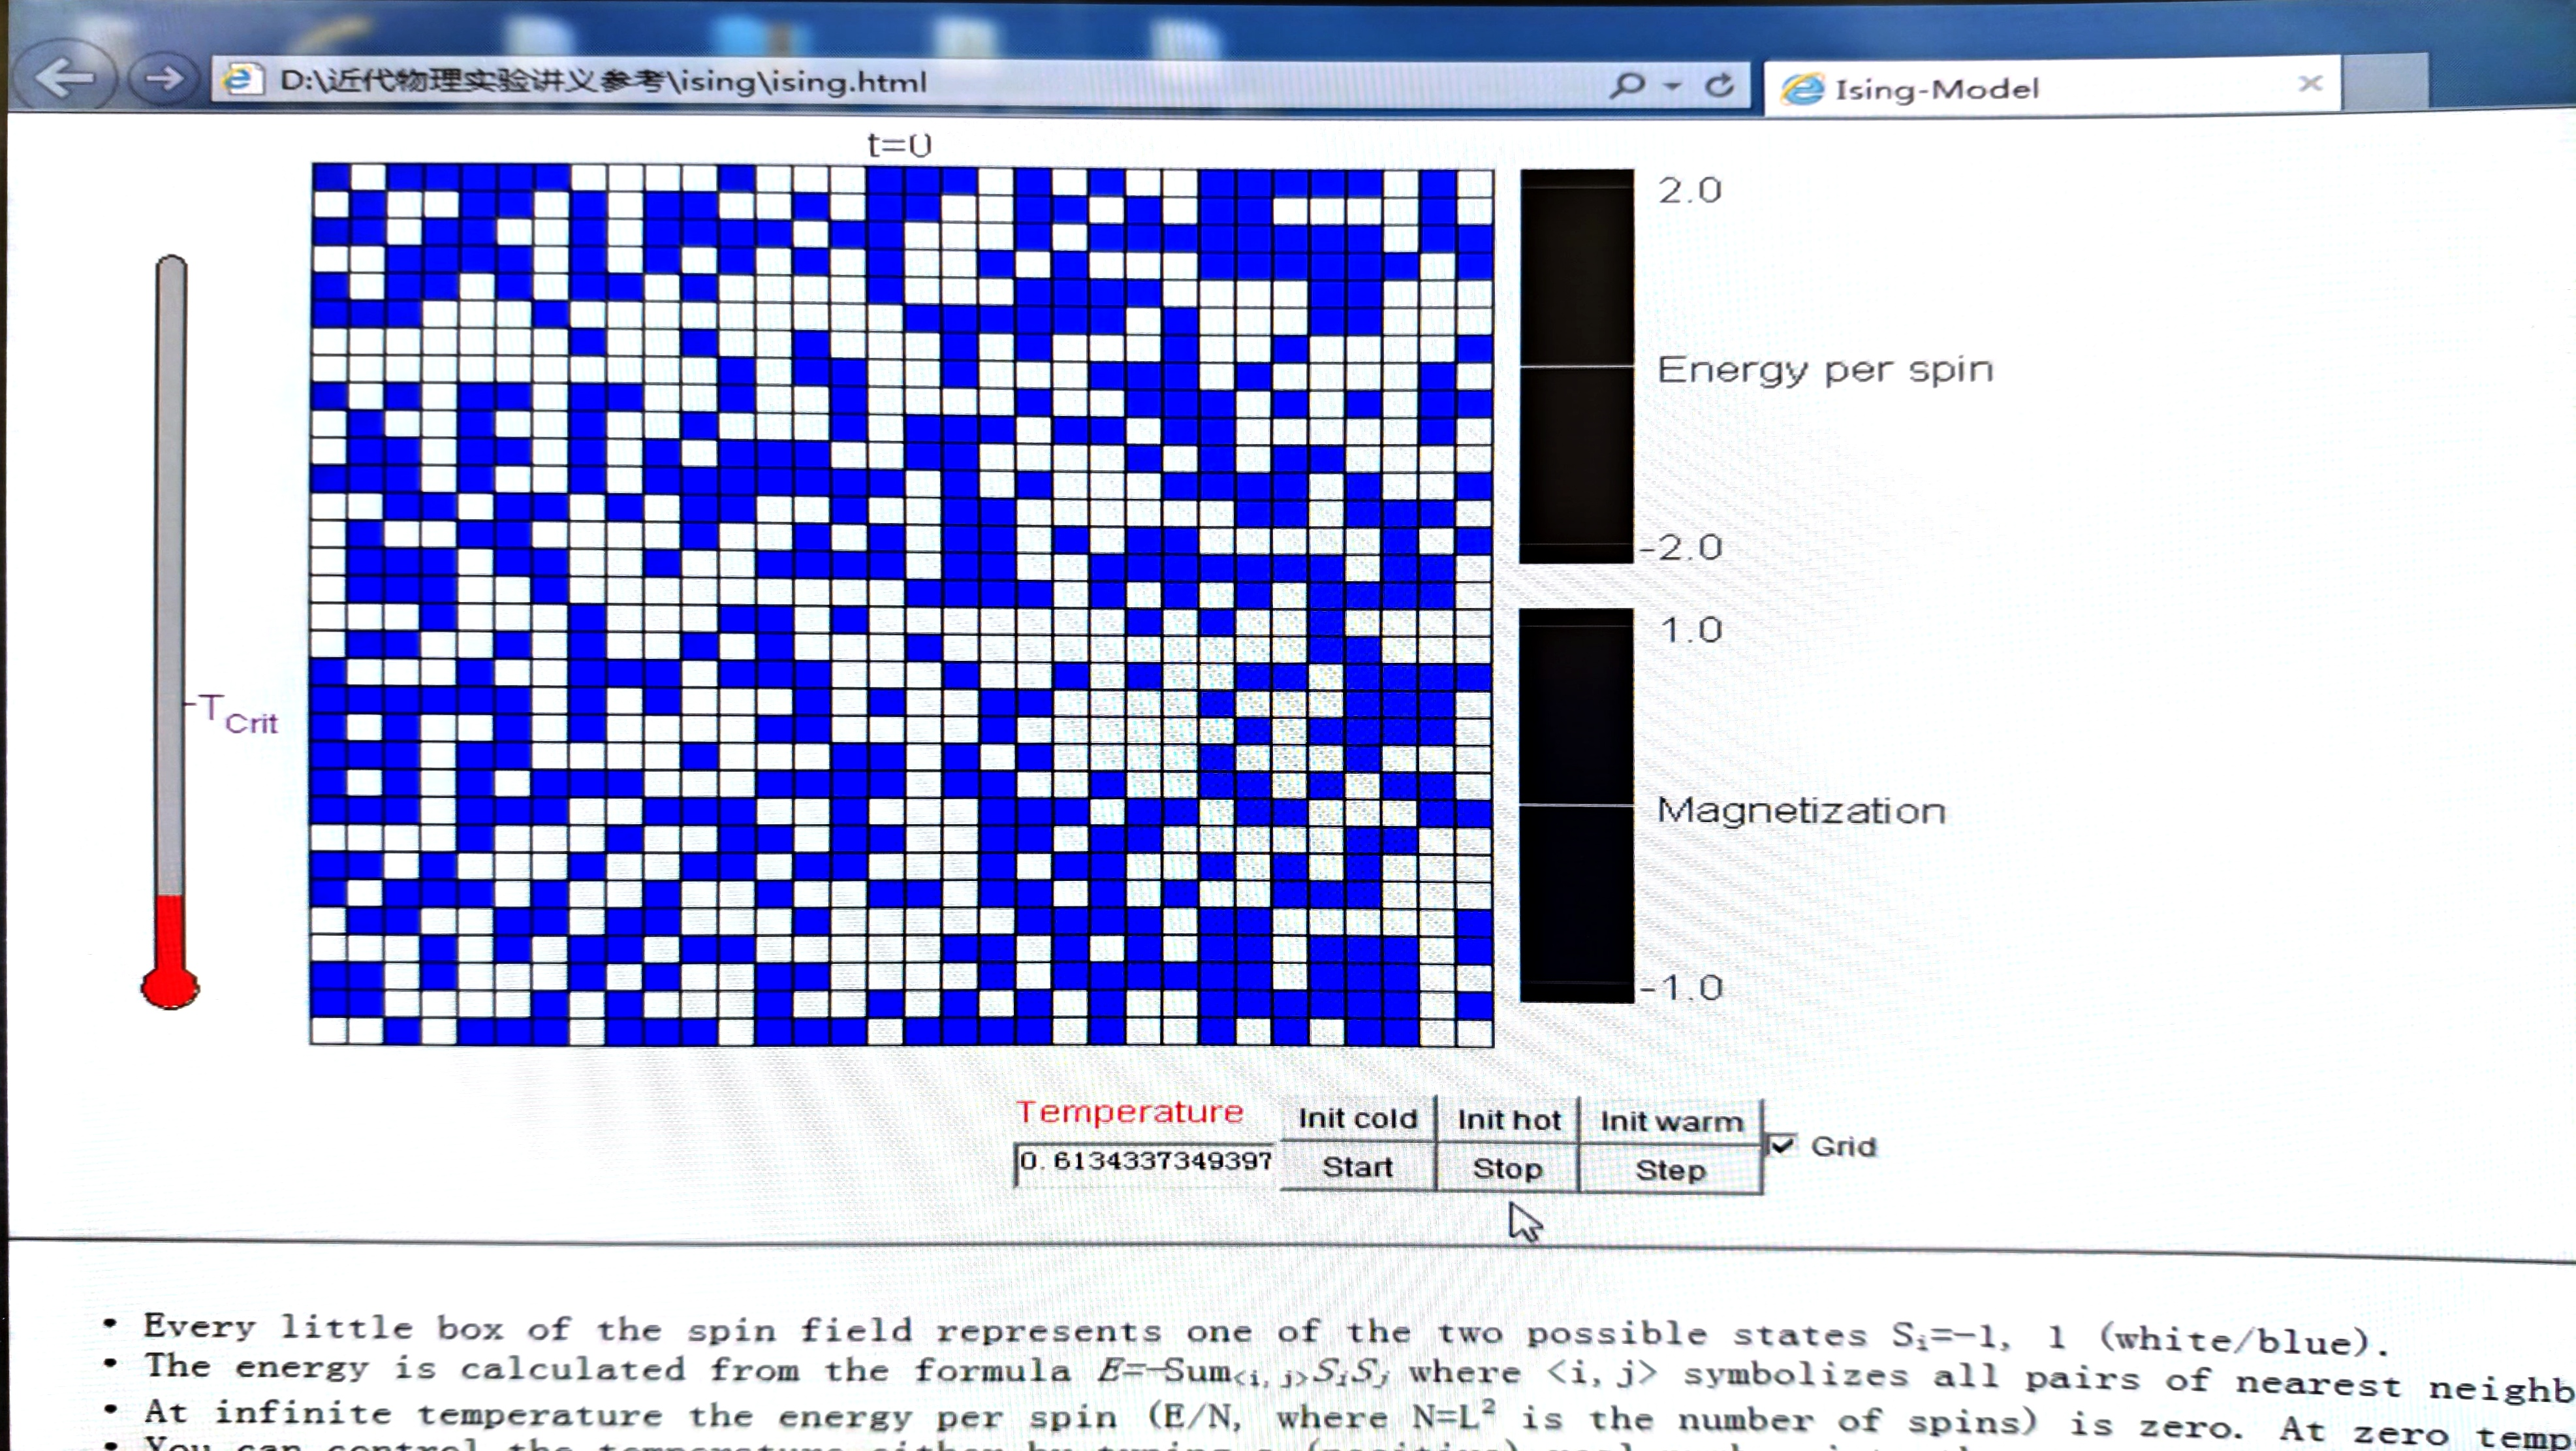
\includegraphics[width=0.6\textwidth]{Figure/fig1.jpg}
        \caption{二维Ising模型蒙特卡罗模拟的软件控制参数界面}
        \label{fig:param_setup}
    \end{figure}
    
    \item \textbf{初始自旋格点态的设置}：初始化二维晶格自旋。图 \ref{fig:initial_states} 分别展示了在不同初设状态（例如高温乱序和低温一致）下的系统随机与统一格点自旋组态。
    \begin{figure}[H]
        \centering
        \begin{subfigure}[b]{0.32\textwidth}
            \centering
            
\includegraphics[width=\textwidth]{Figure/fig2.jpg}
            \caption{低温完全一致有序态}
        \end{subfigure}
        \hfill
        \begin{subfigure}[b]{0.32\textwidth}
            \centering
            
\includegraphics[width=\textwidth]{Figure/fig3.jpg}
            \caption{高温均匀混合随机态}
        \end{subfigure}
        \hfill
        \begin{subfigure}[b]{0.32\textwidth}
            \centering
            
\includegraphics[width=\textwidth]{Figure/fig4.jpg}
            \caption{亚稳态混合组态}
        \end{subfigure}
        \caption{Ising模型模拟程序自选初始状态设置与格点构型界面}
        \label{fig:initial_states}
    \end{figure}

    \item \textbf{高温无序态下的自旋涨落演化}：将系统温度设定在远高于临界相变点（$T_c \approx 2.27$）的高温区（如 $T = 3.5$），运行 Metropolis 算法。图 \ref{fig:high_temp_evolve} 显示了高温状态下，自旋受剧烈热噪声干扰、呈现细碎分布的快速随机随机翻转过程。
    \begin{figure}[H]
        \centering
        \begin{subfigure}[b]{0.32\textwidth}
            \centering
            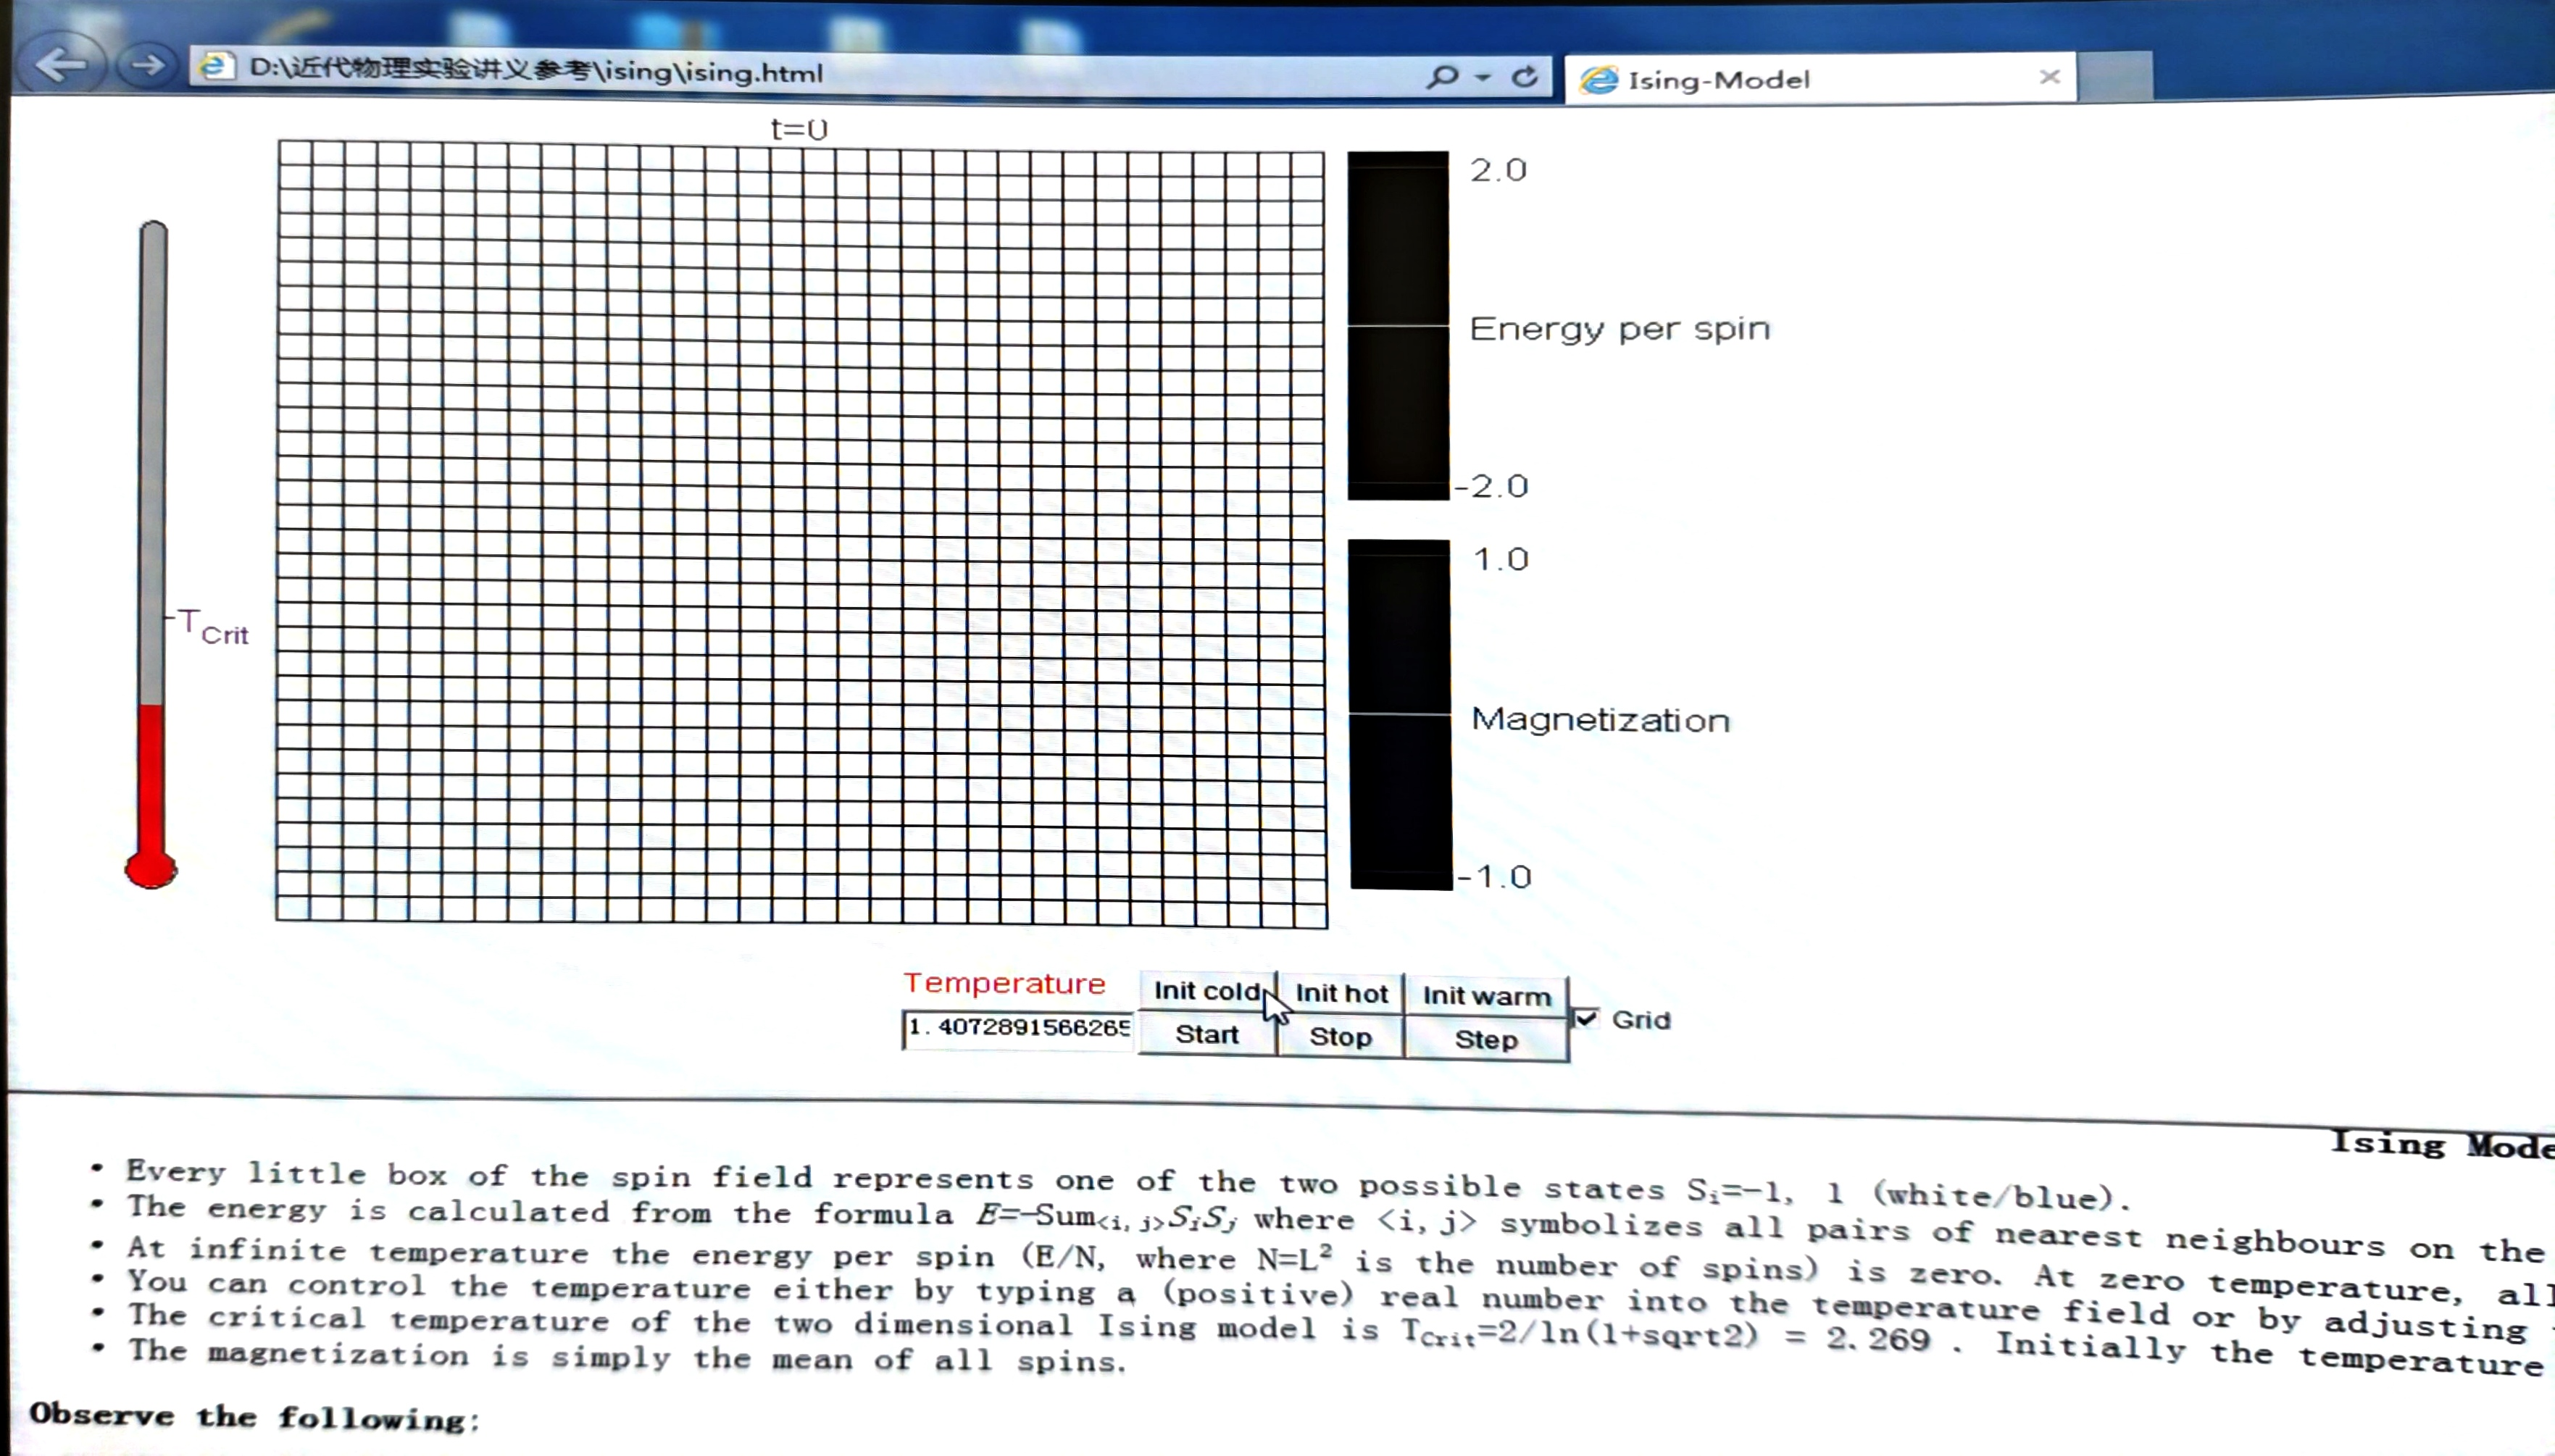
\includegraphics[width=\textwidth]{Figure/fig5.jpg}
            \caption{高温演化初始阶段}
        \end{subfigure}
        \hfill
        \begin{subfigure}[b]{0.32\textwidth}
            \centering
            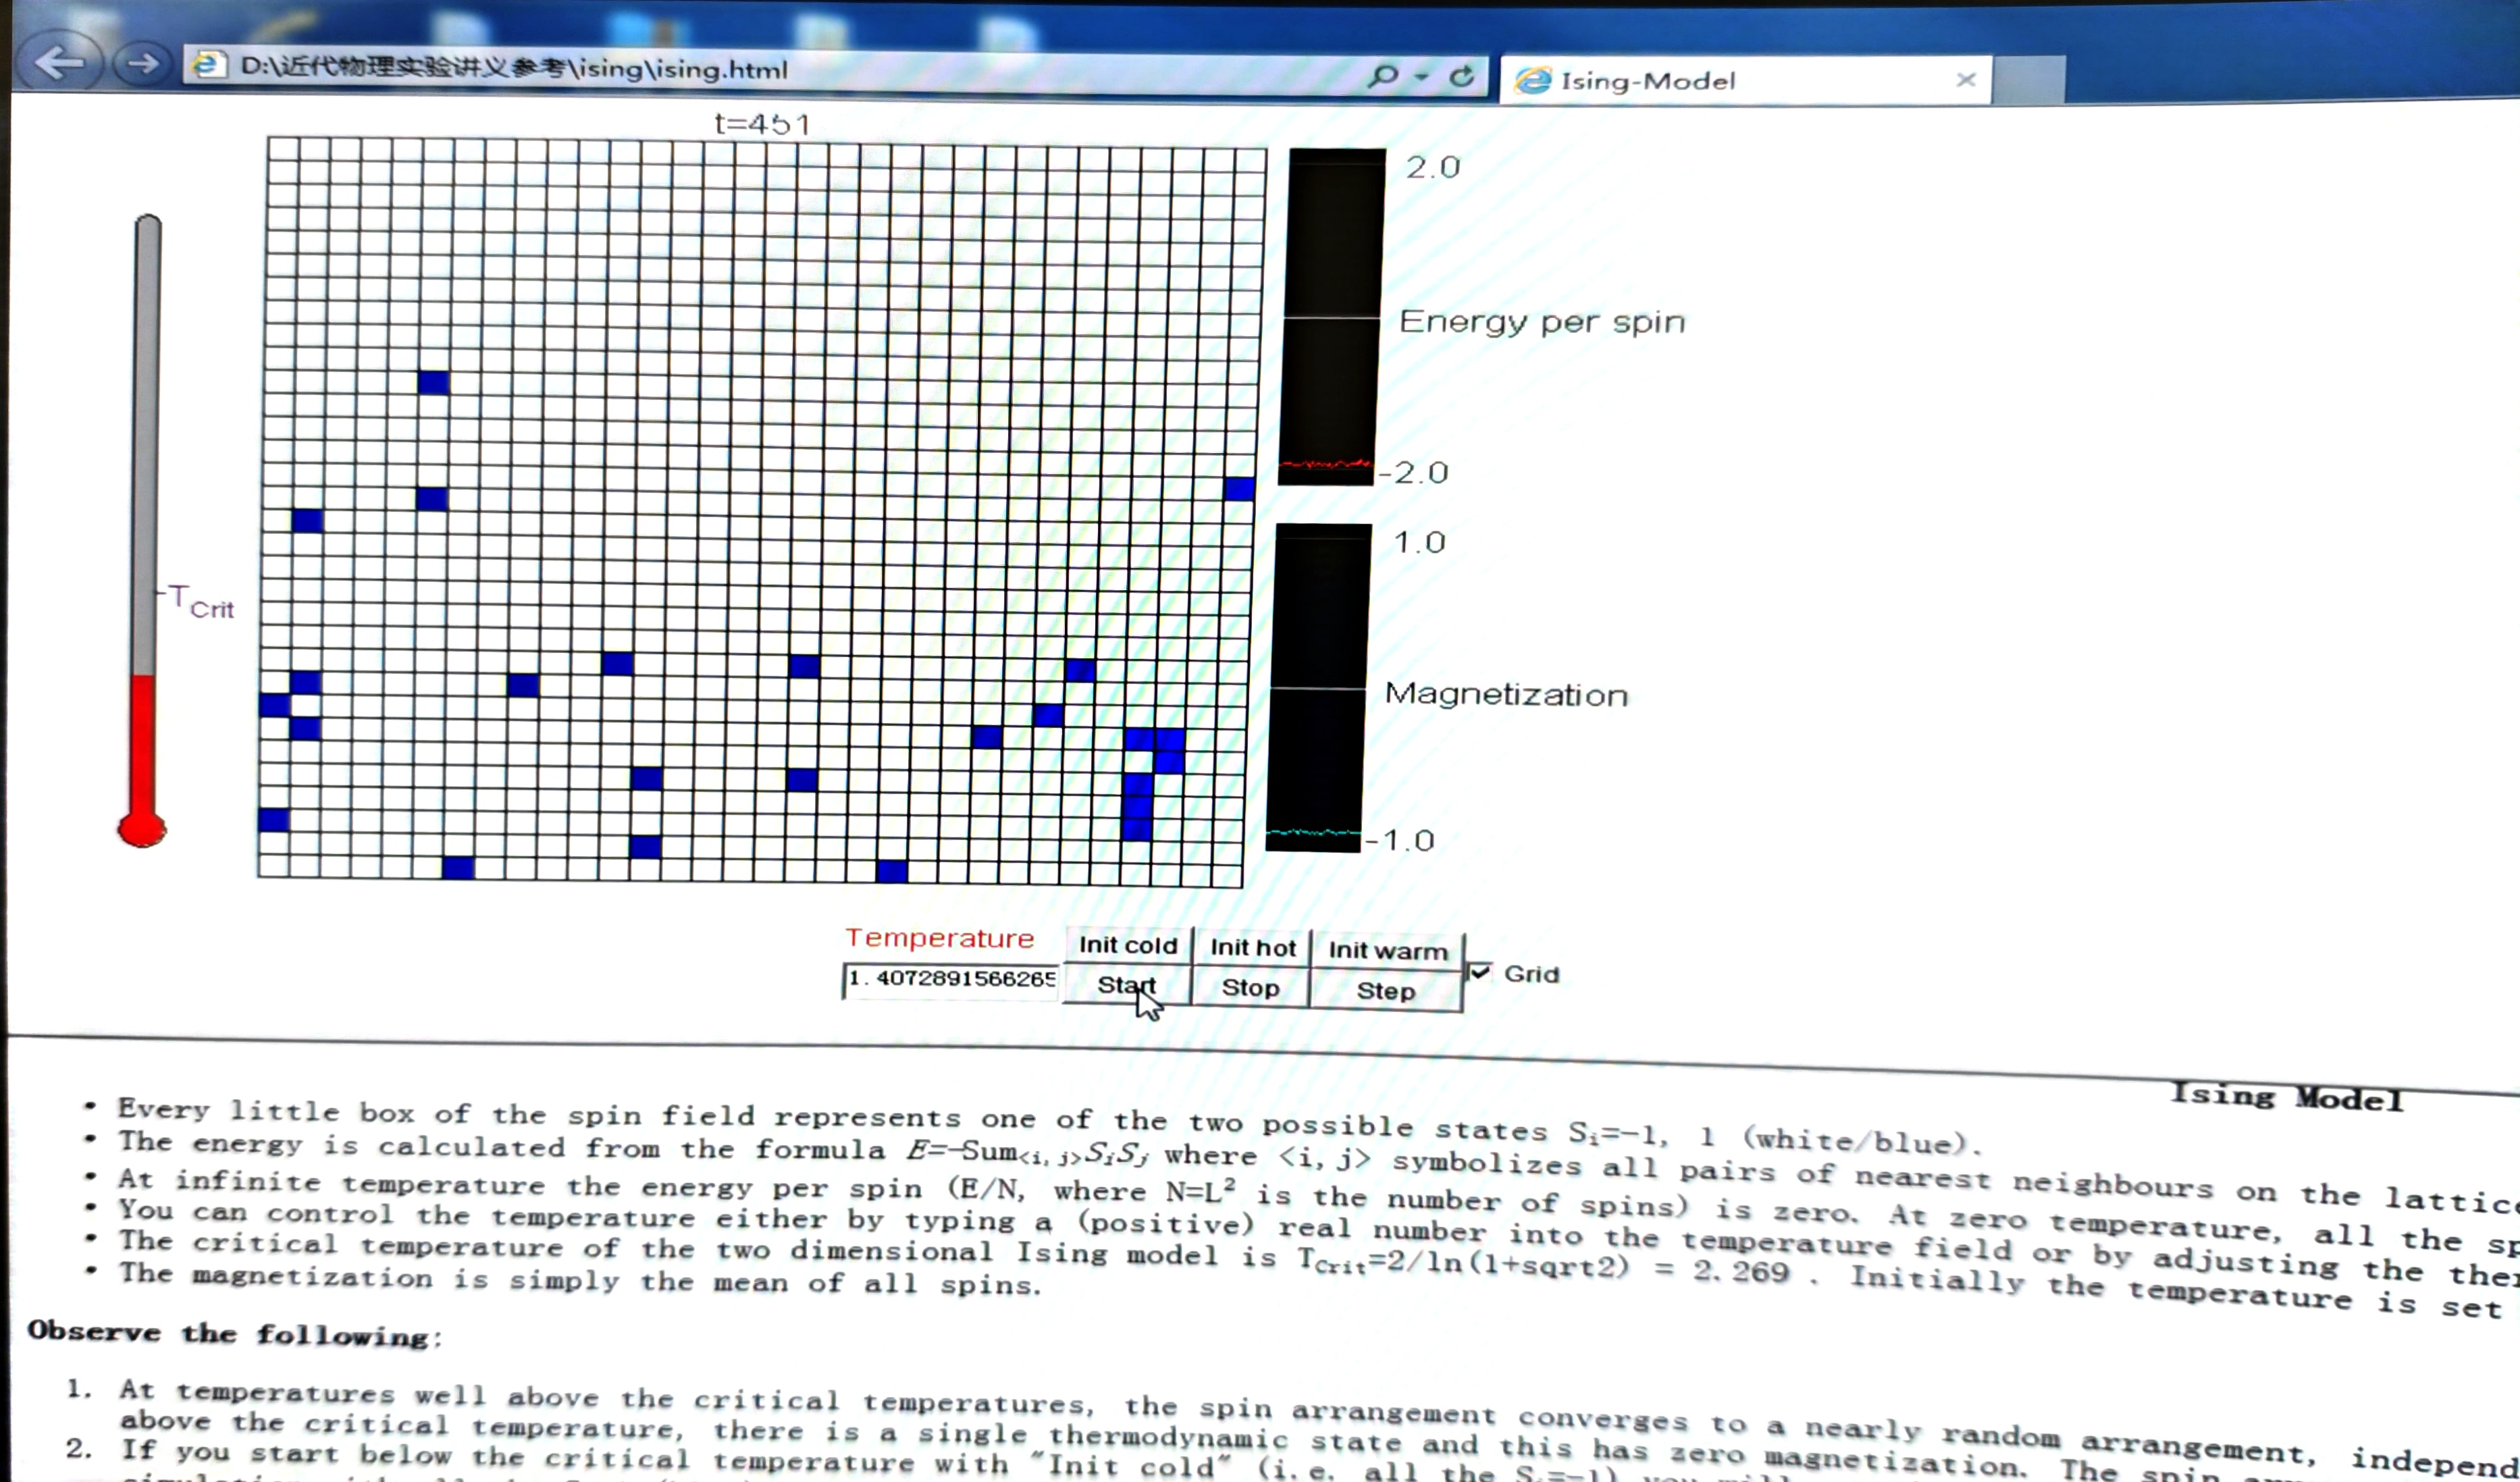
\includegraphics[width=\textwidth]{Figure/fig6.jpg}
            \caption{高温演化中间阶段}
        \end{subfigure}
        \hfill
        \begin{subfigure}[b]{0.32\textwidth}
            \centering
            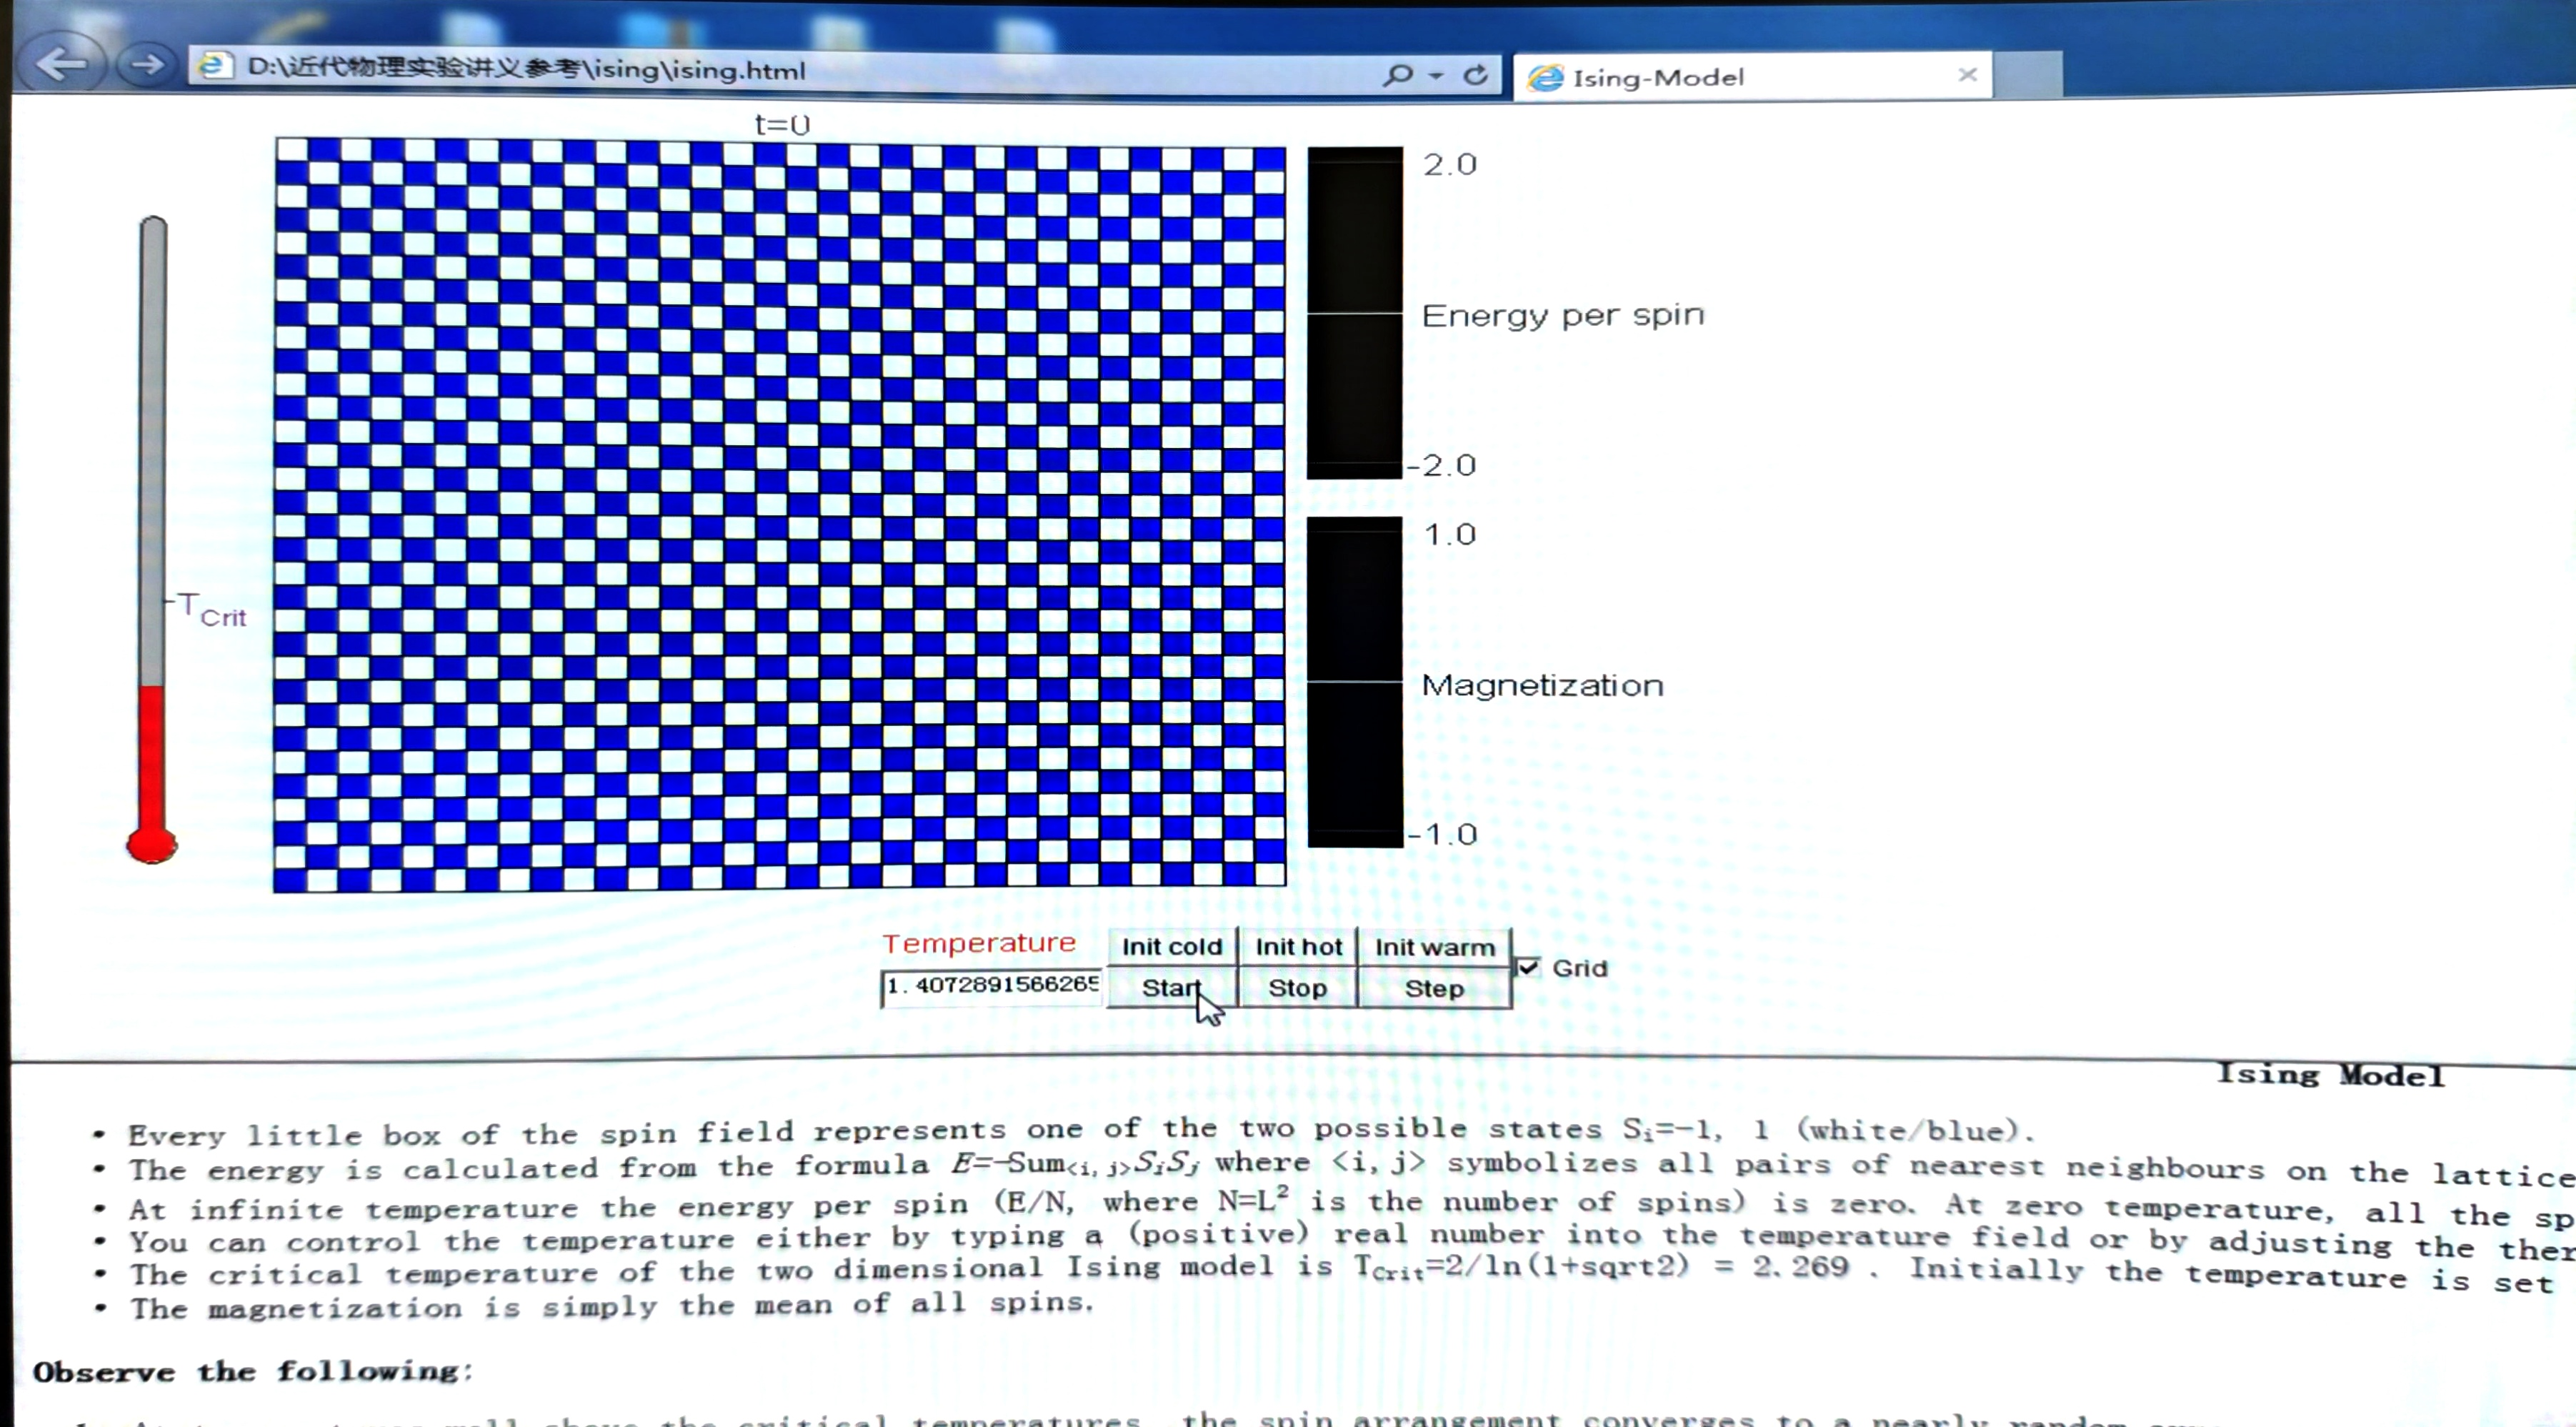
\includegraphics[width=\textwidth]{Figure/fig7.jpg}
            \caption{高温演化热平衡态}
        \end{subfigure}
        \caption{高温无序相（$T > T_c$）自旋分布随蒙特卡罗步数的实时随机演化图像}
        \label{fig:high_temp_evolve}
    \end{figure}

    \item \textbf{临界温度点附近的自旋畴演化}：将温度设定在临界温度附近（$T = 2.27$），运行算法。图 \ref{fig:critical_temp_evolve} 展现了在临界相变点处，系统关联长度发散，出现大块大块、分形般的自旋畴（自旋向上与向下的畴块共存且剧烈涨落）。
    \begin{figure}[H]
        \centering
        \begin{subfigure}[b]{0.24\textwidth}
            \centering
            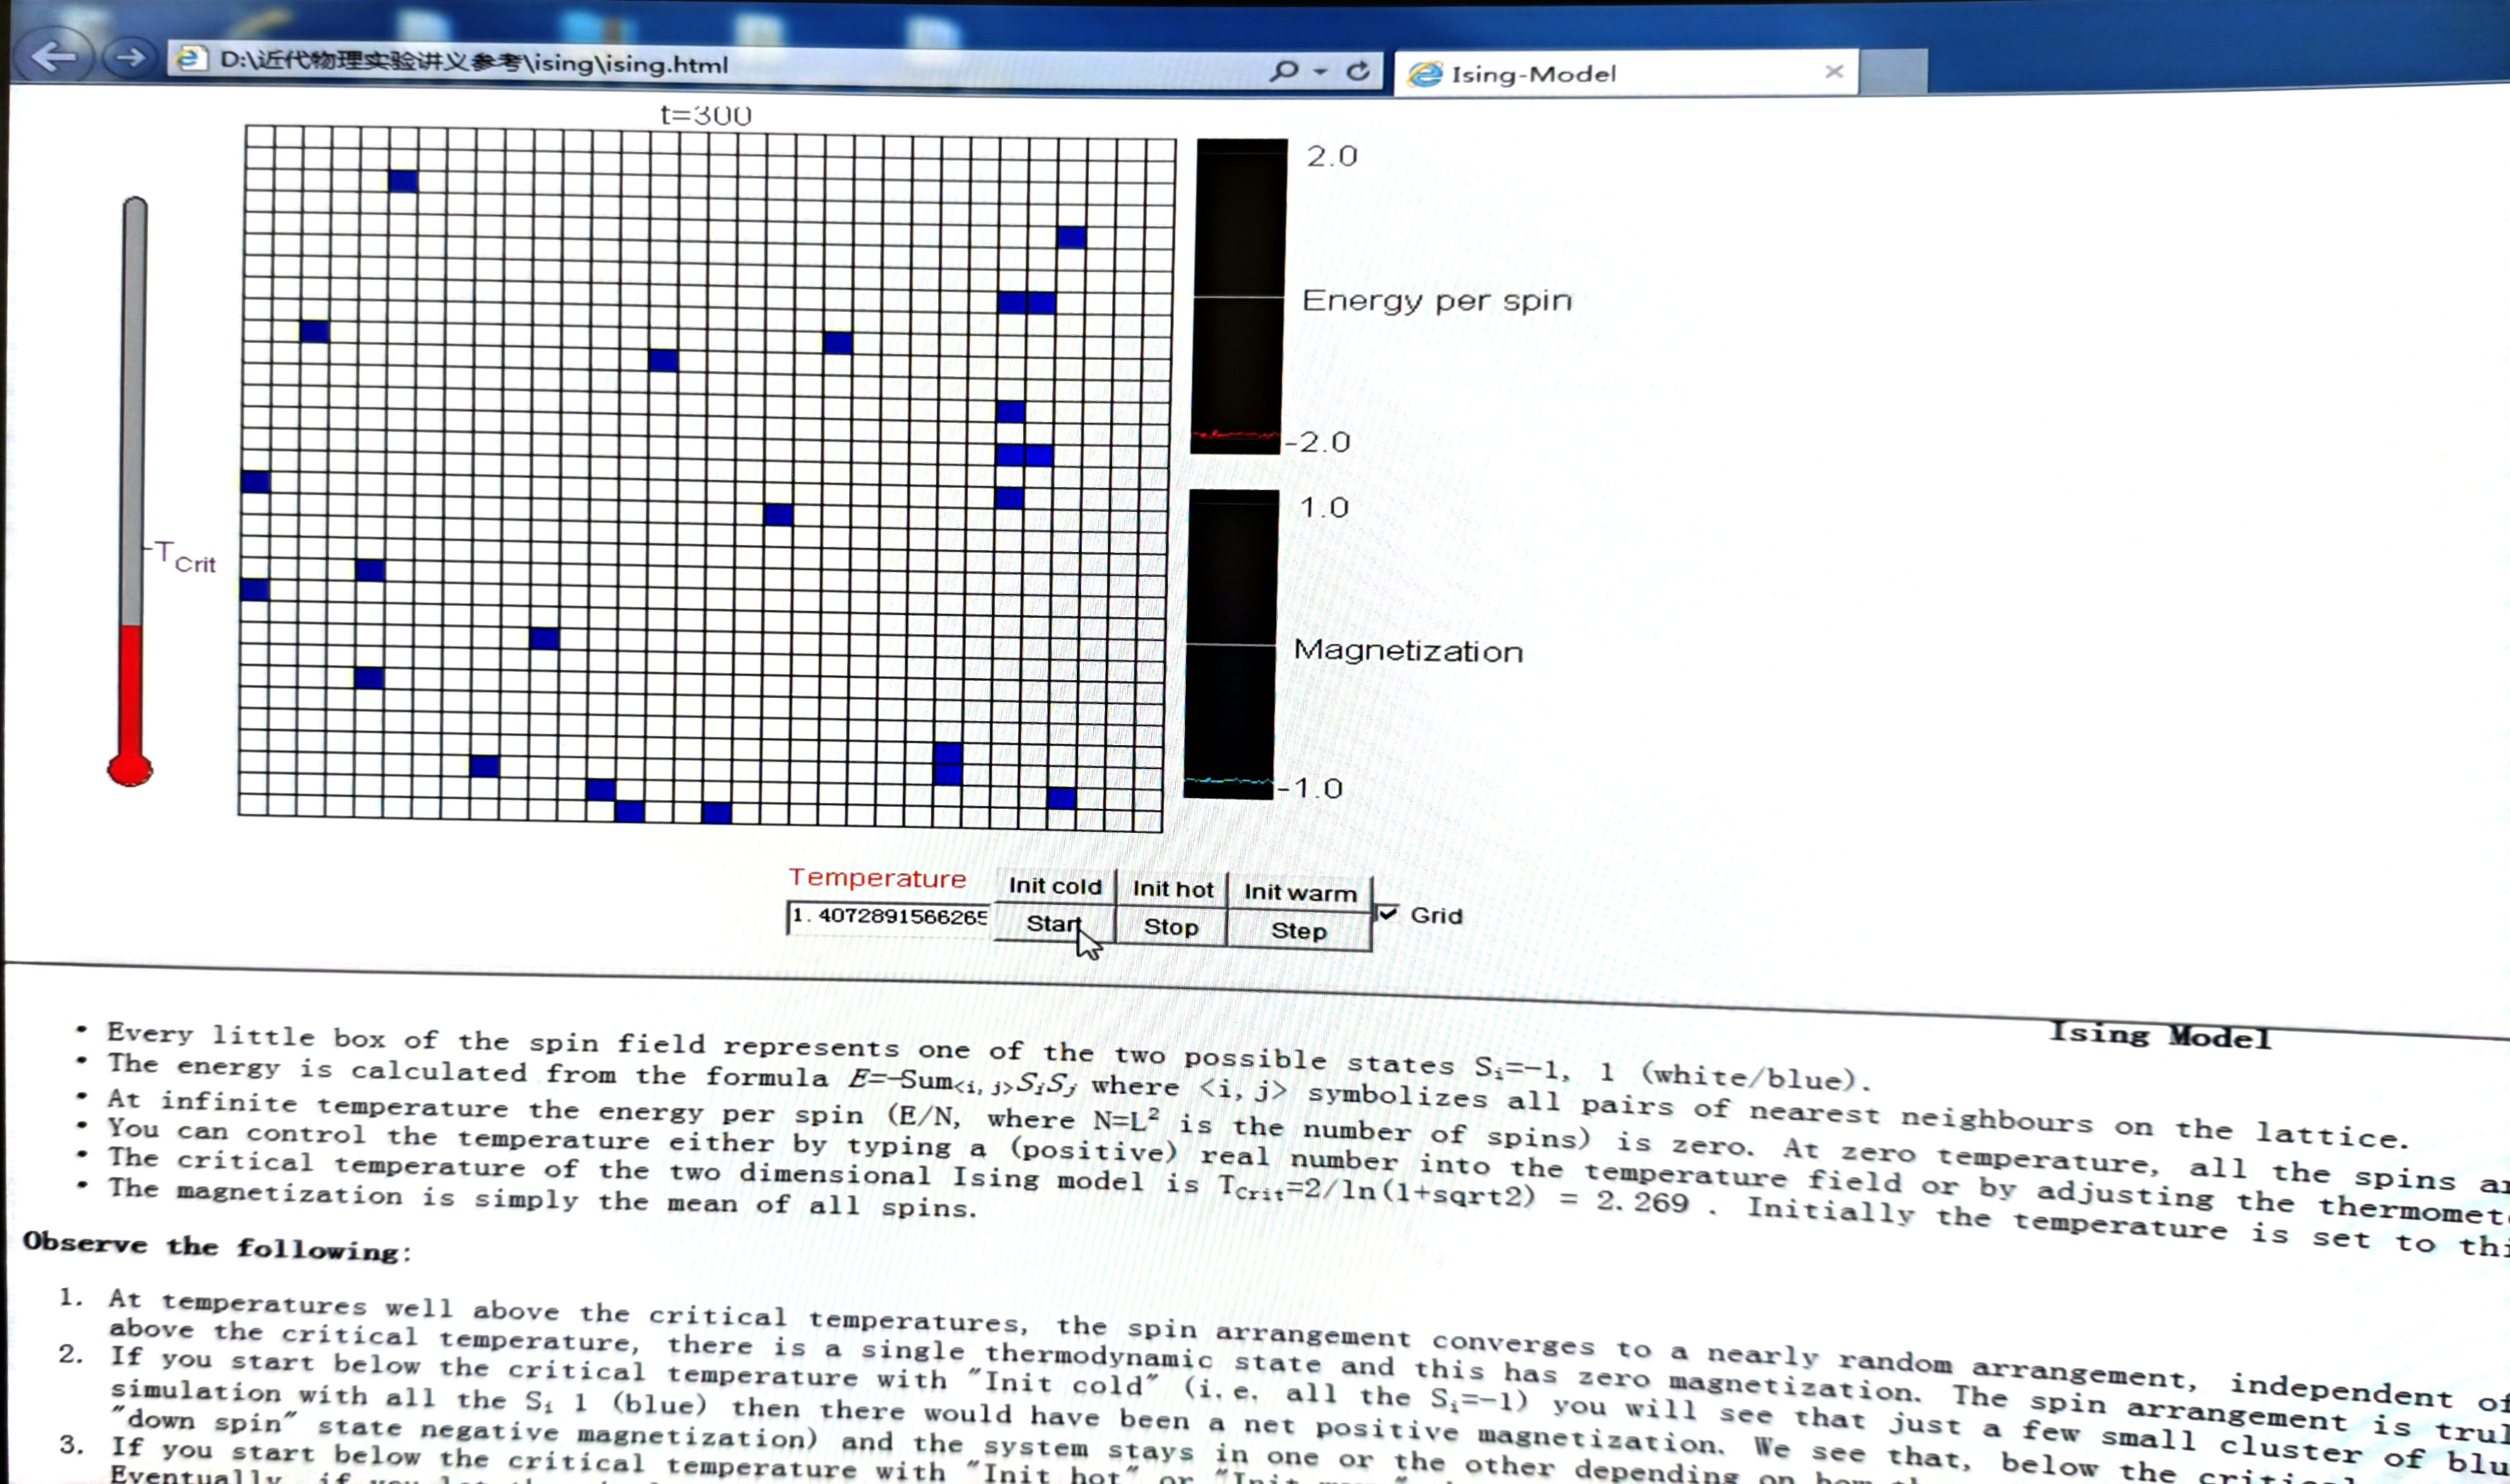
\includegraphics[width=\textwidth]{Figure/fig8.jpg}
            \caption{演化第100步}
        \end{subfigure}
        \hfill
        \begin{subfigure}[b]{0.24\textwidth}
            \centering
            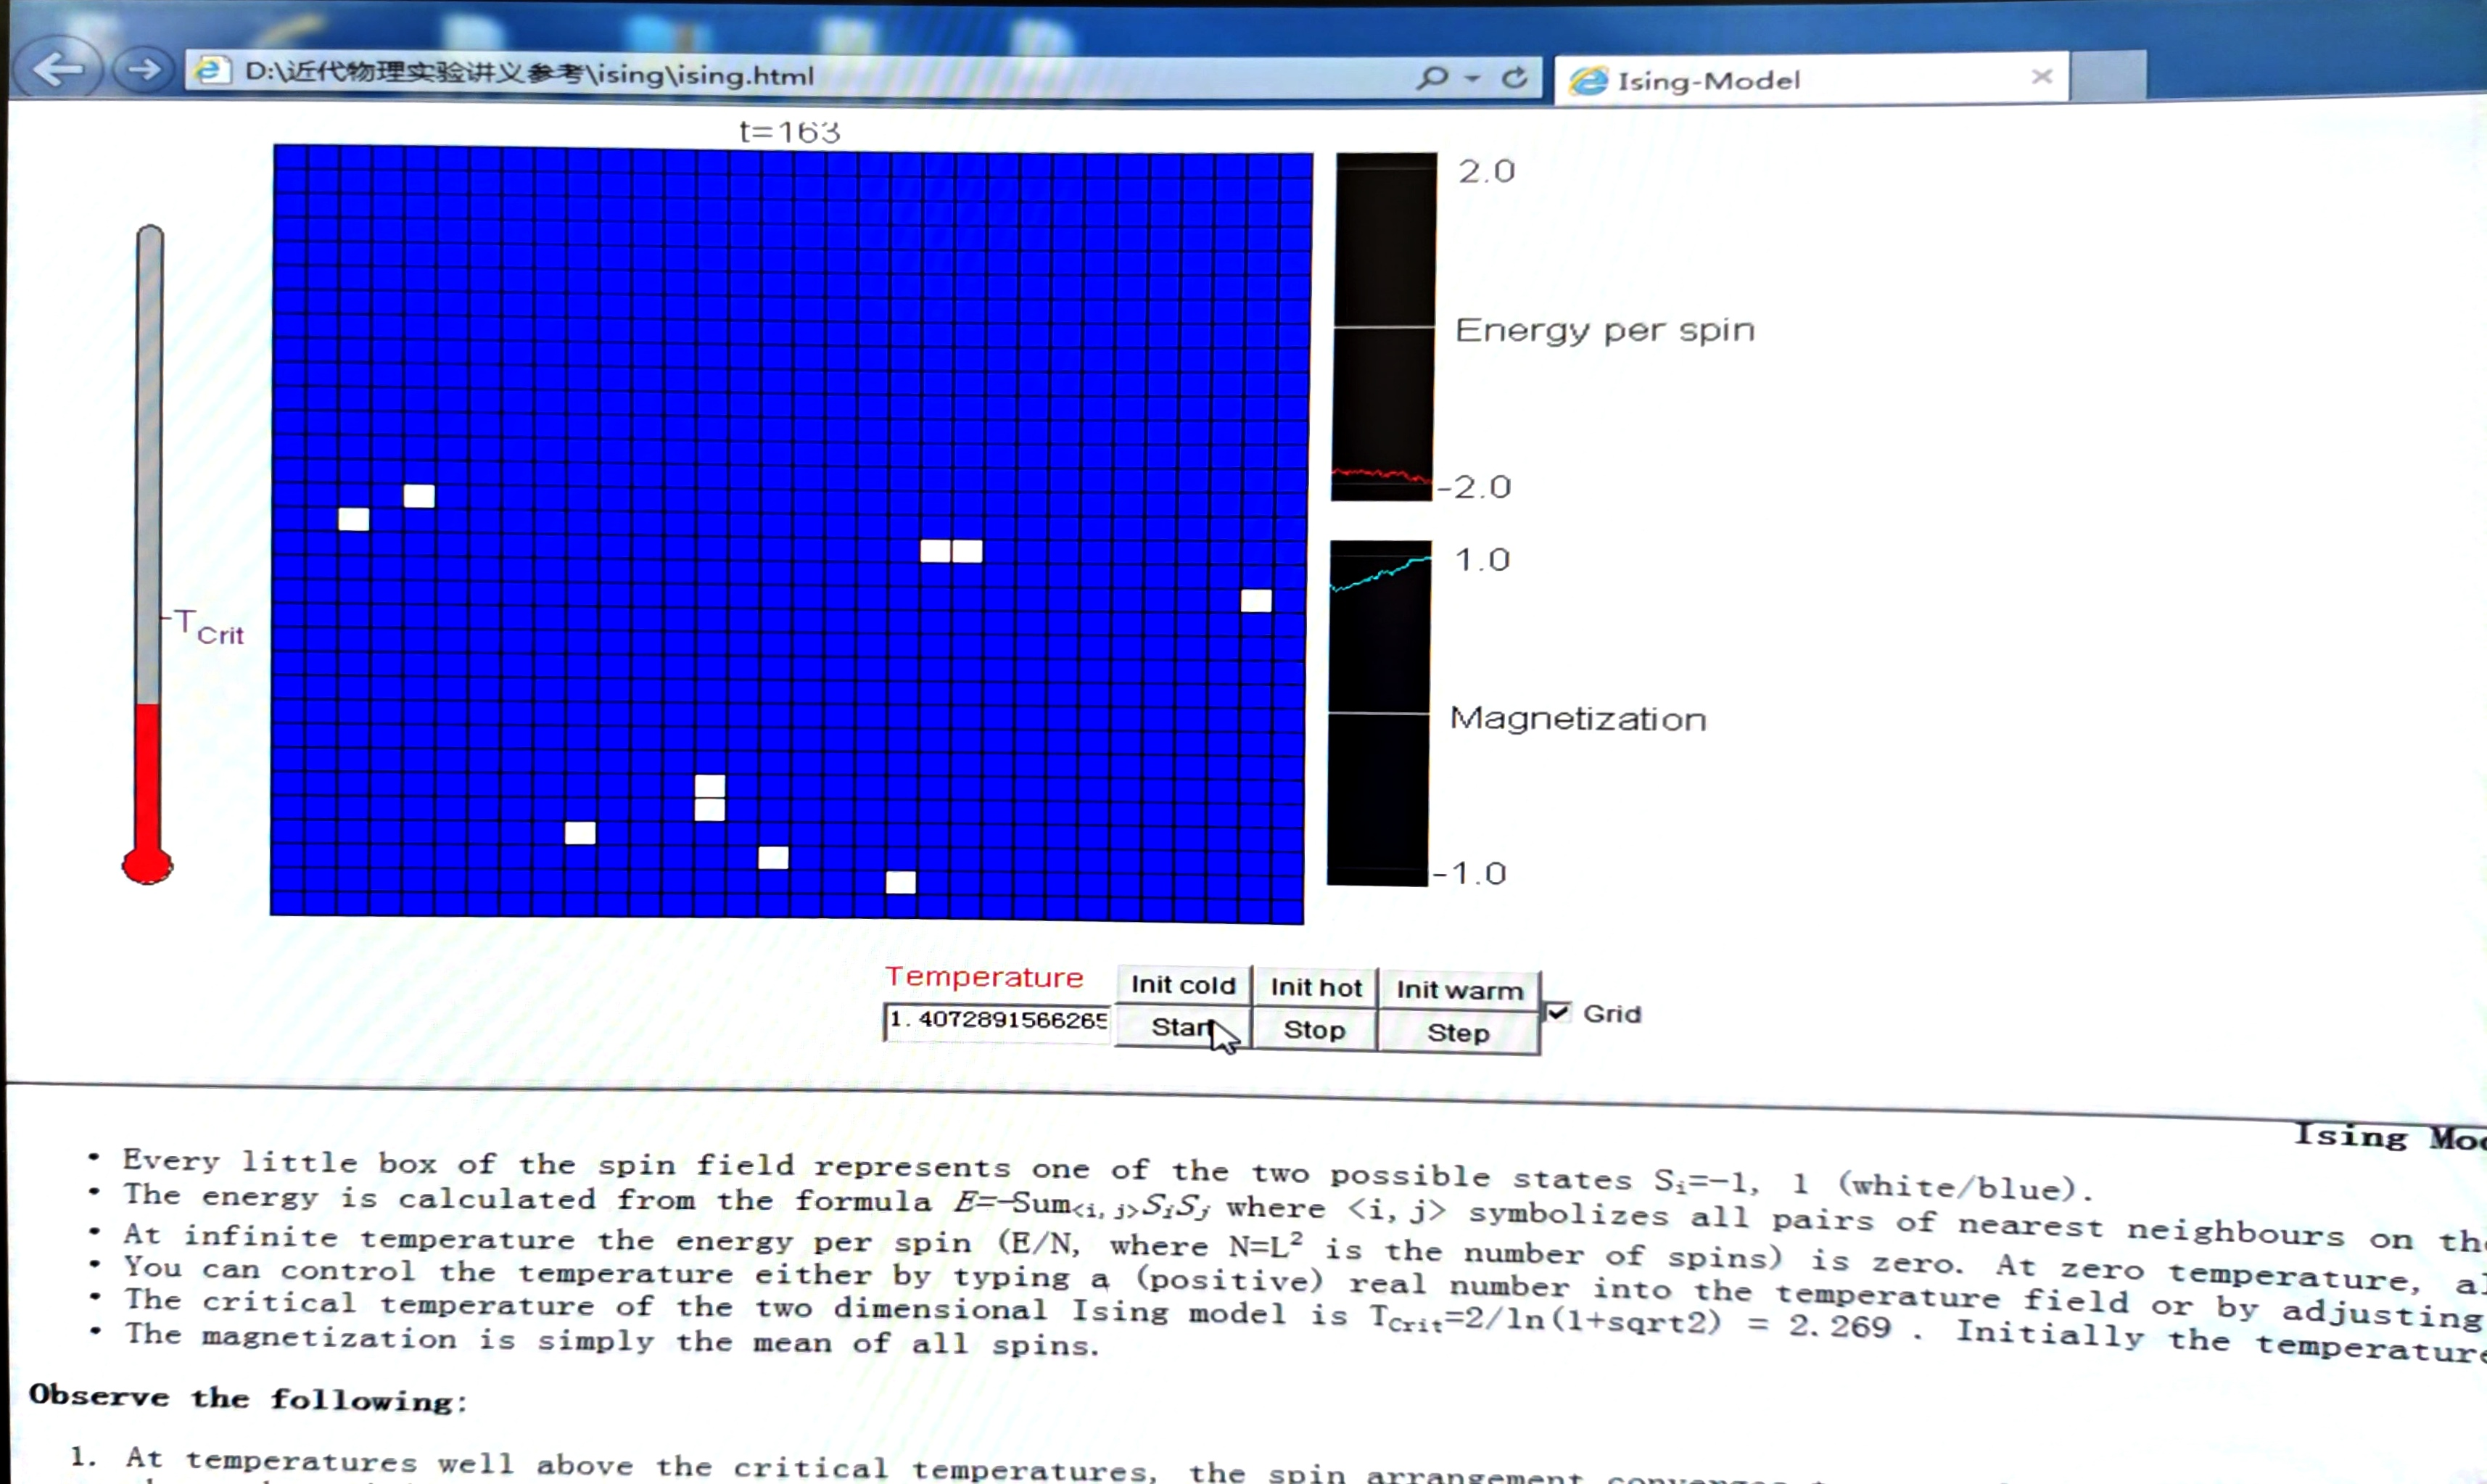
\includegraphics[width=\textwidth]{Figure/fig9.jpg}
            \caption{演化第300步}
        \end{subfigure}
        \hfill
        \begin{subfigure}[b]{0.24\textwidth}
            \centering
            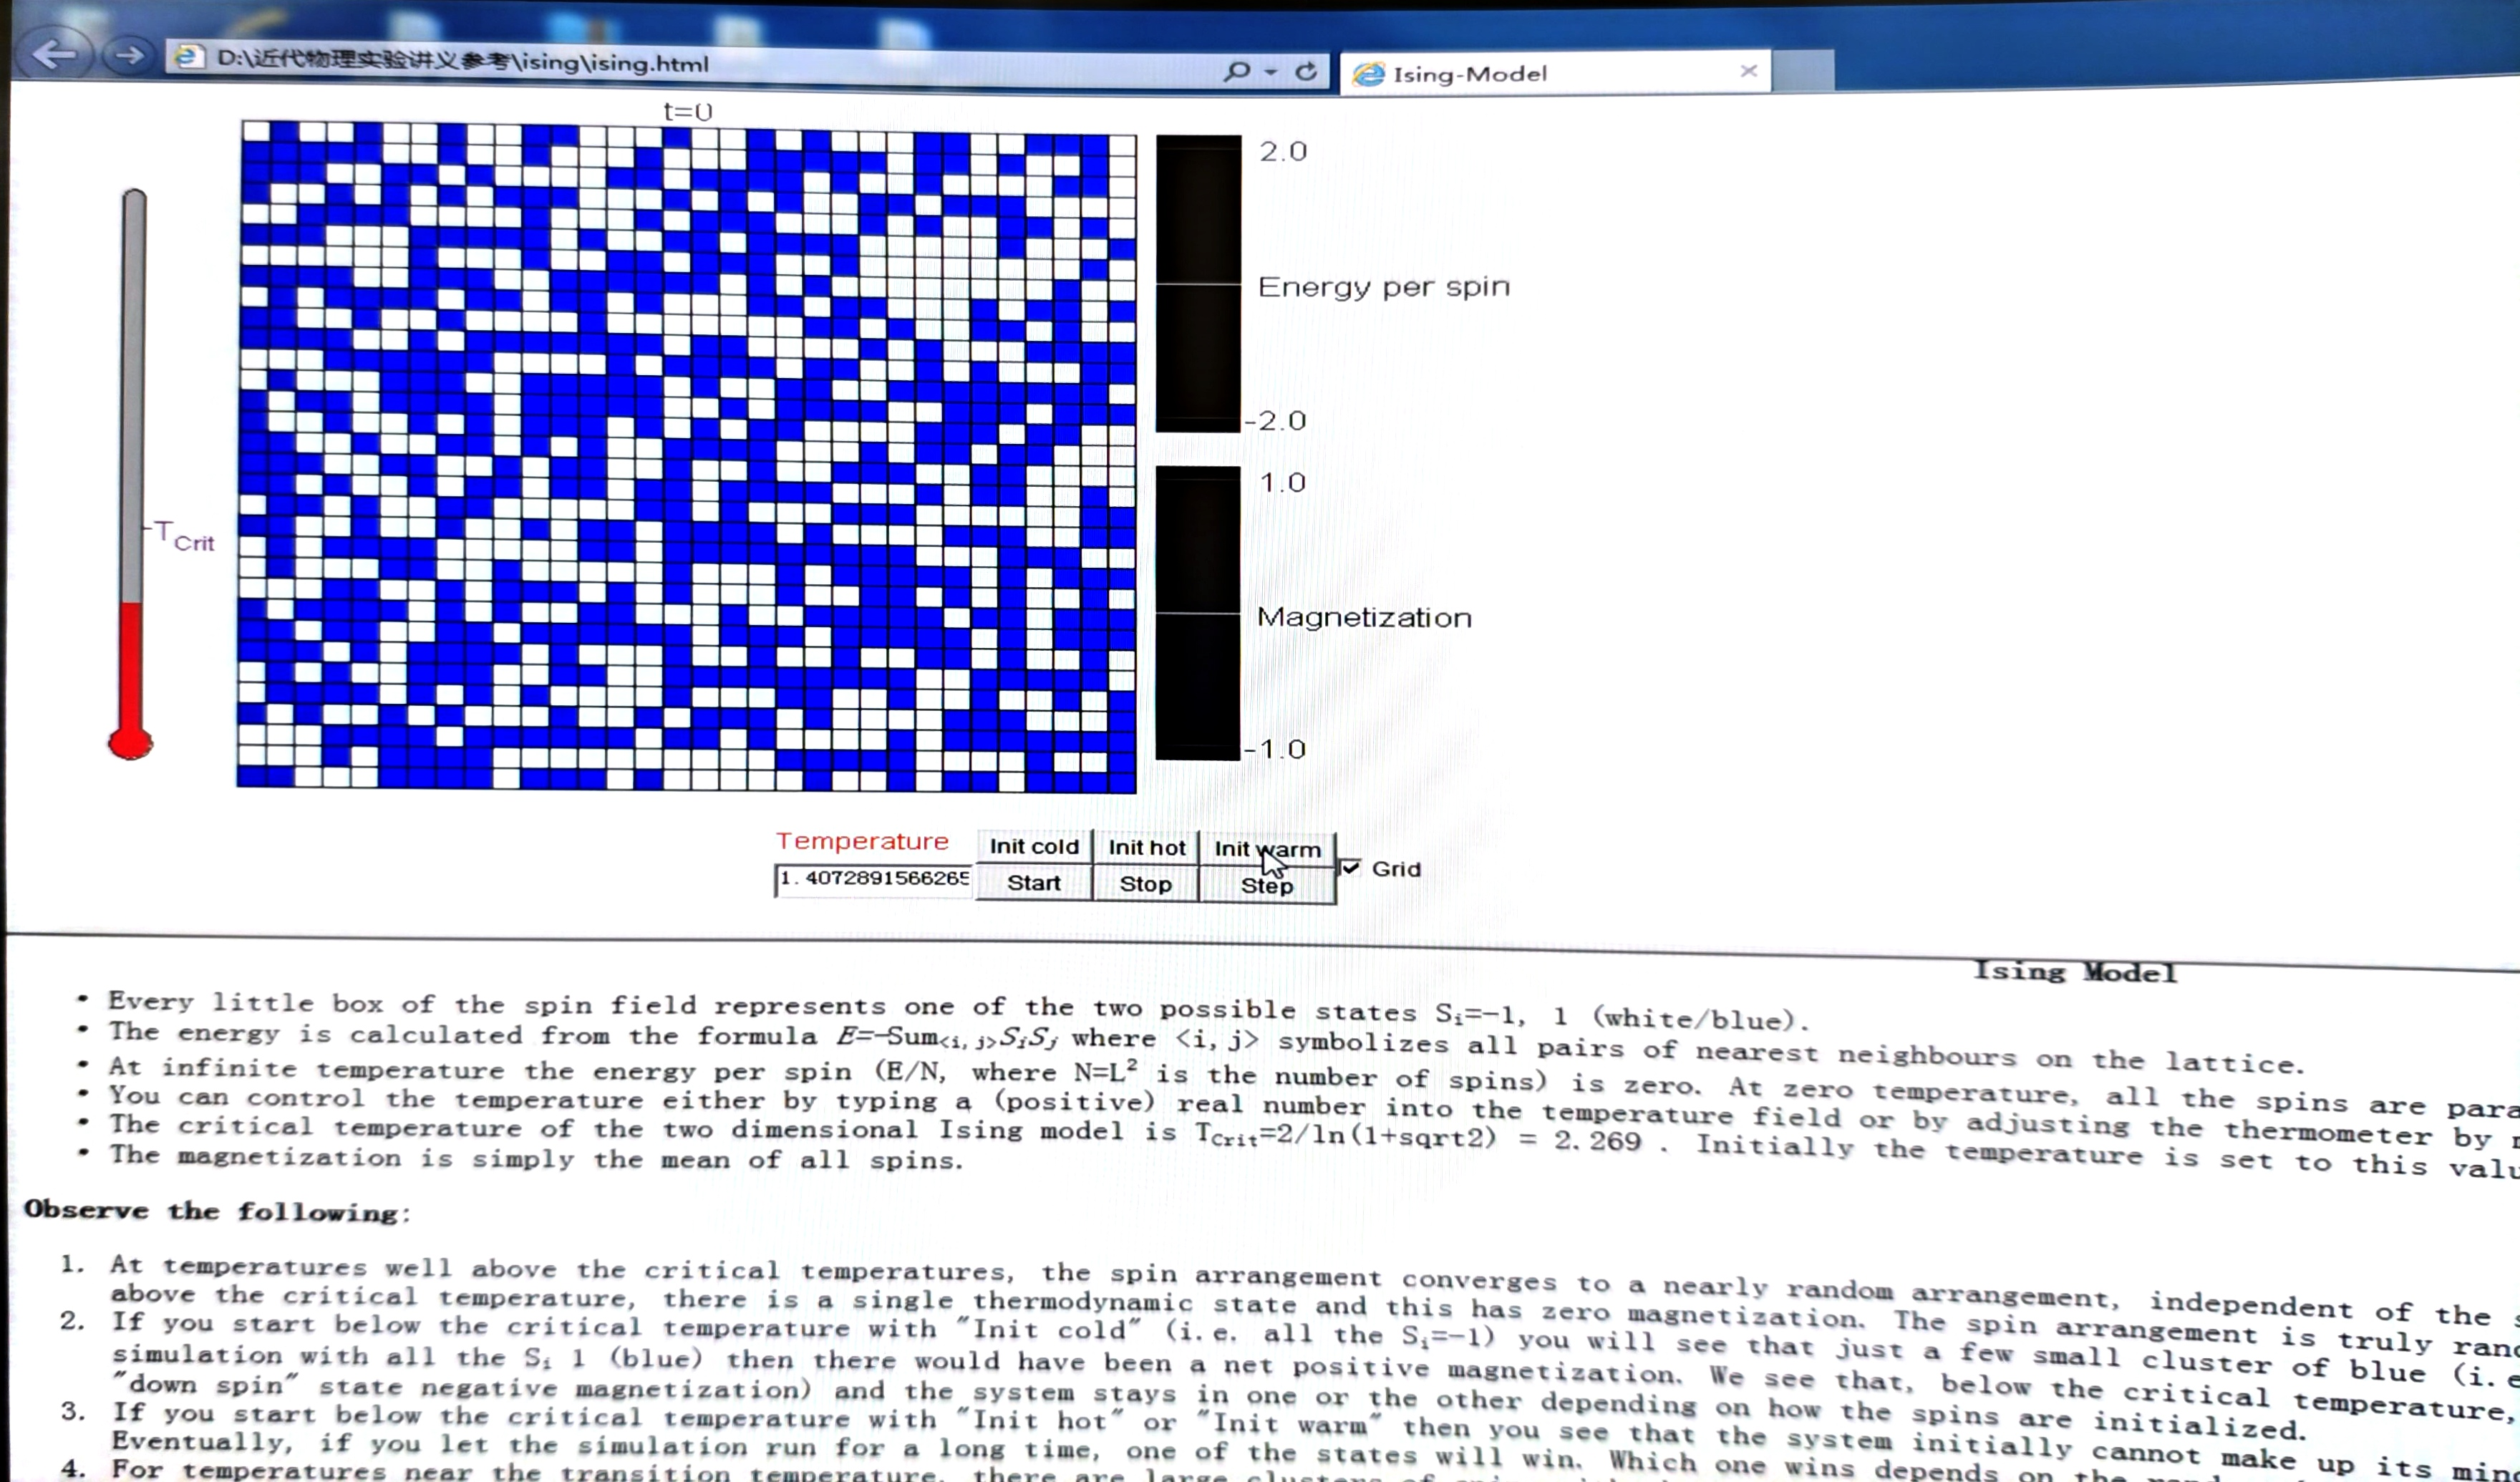
\includegraphics[width=\textwidth]{Figure/fig10.jpg}
            \caption{演化第800步}
        \end{subfigure}
        \hfill
        \begin{subfigure}[b]{0.24\textwidth}
            \centering
            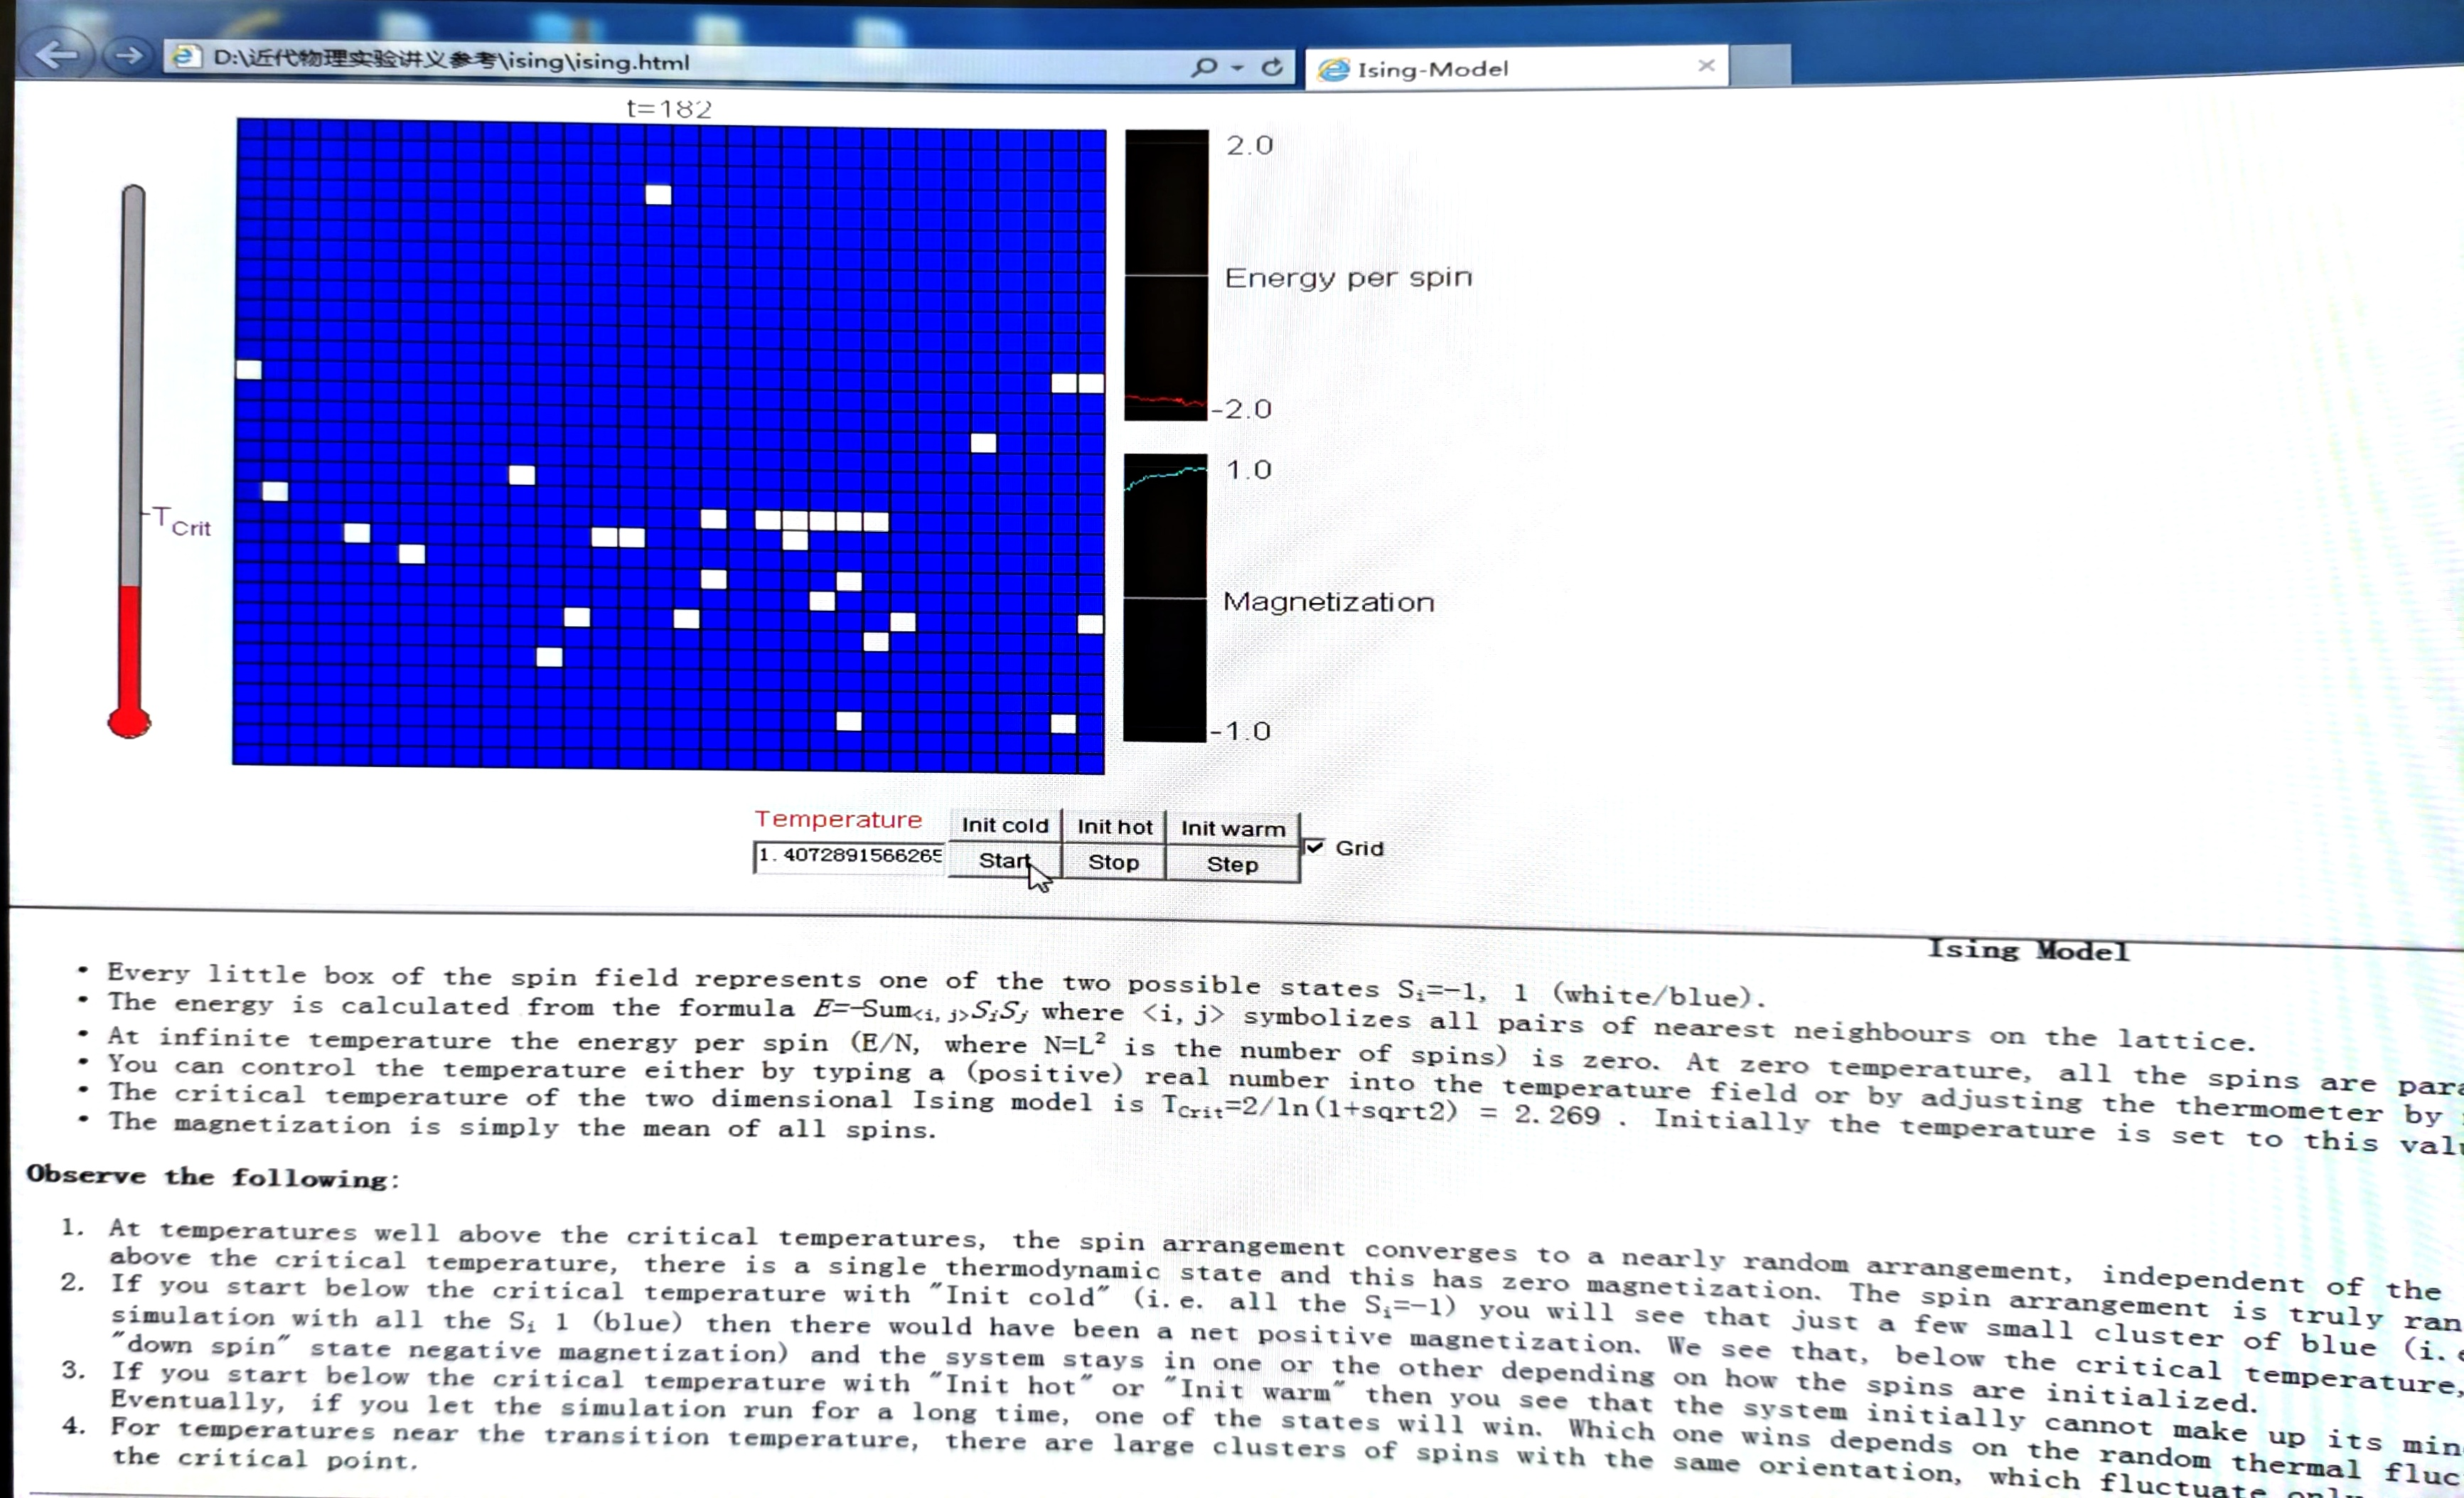
\includegraphics[width=\textwidth]{Figure/fig11.jpg}
            \caption{临界热平衡态}
        \end{subfigure}
        \caption{临界区（$T \approx T_c$）分形自旋畴共存随蒙特卡罗步数的实时演化图像}
        \label{fig:critical_temp_evolve}
    \end{figure}
\end{enumerate}

\section{实验数据处理}

本实验通过长时间蒙特卡罗采样，获取了在不同晶格尺寸（$L=16, 32, 64$）及不同温度下的热力学物理数据，并对实验结果进行了系统分析。

\subsection{低温有序相下的自旋演化}
在低温区（$T < T_c$），自旋之间的近邻相互作用（能量约束）强于热运动的随机涨落。图 \ref{fig:low_temp_evolve} 展示了在低温下系统如何快速从无序态凝聚到自发磁化的有序态。可见，系统内部逐渐合并出极大型的单一自旋区域（自发磁化区），直至几乎所有自旋平行排列。
\begin{figure}[H]
    \centering
    \begin{subfigure}[b]{0.32\textwidth}
        \centering
        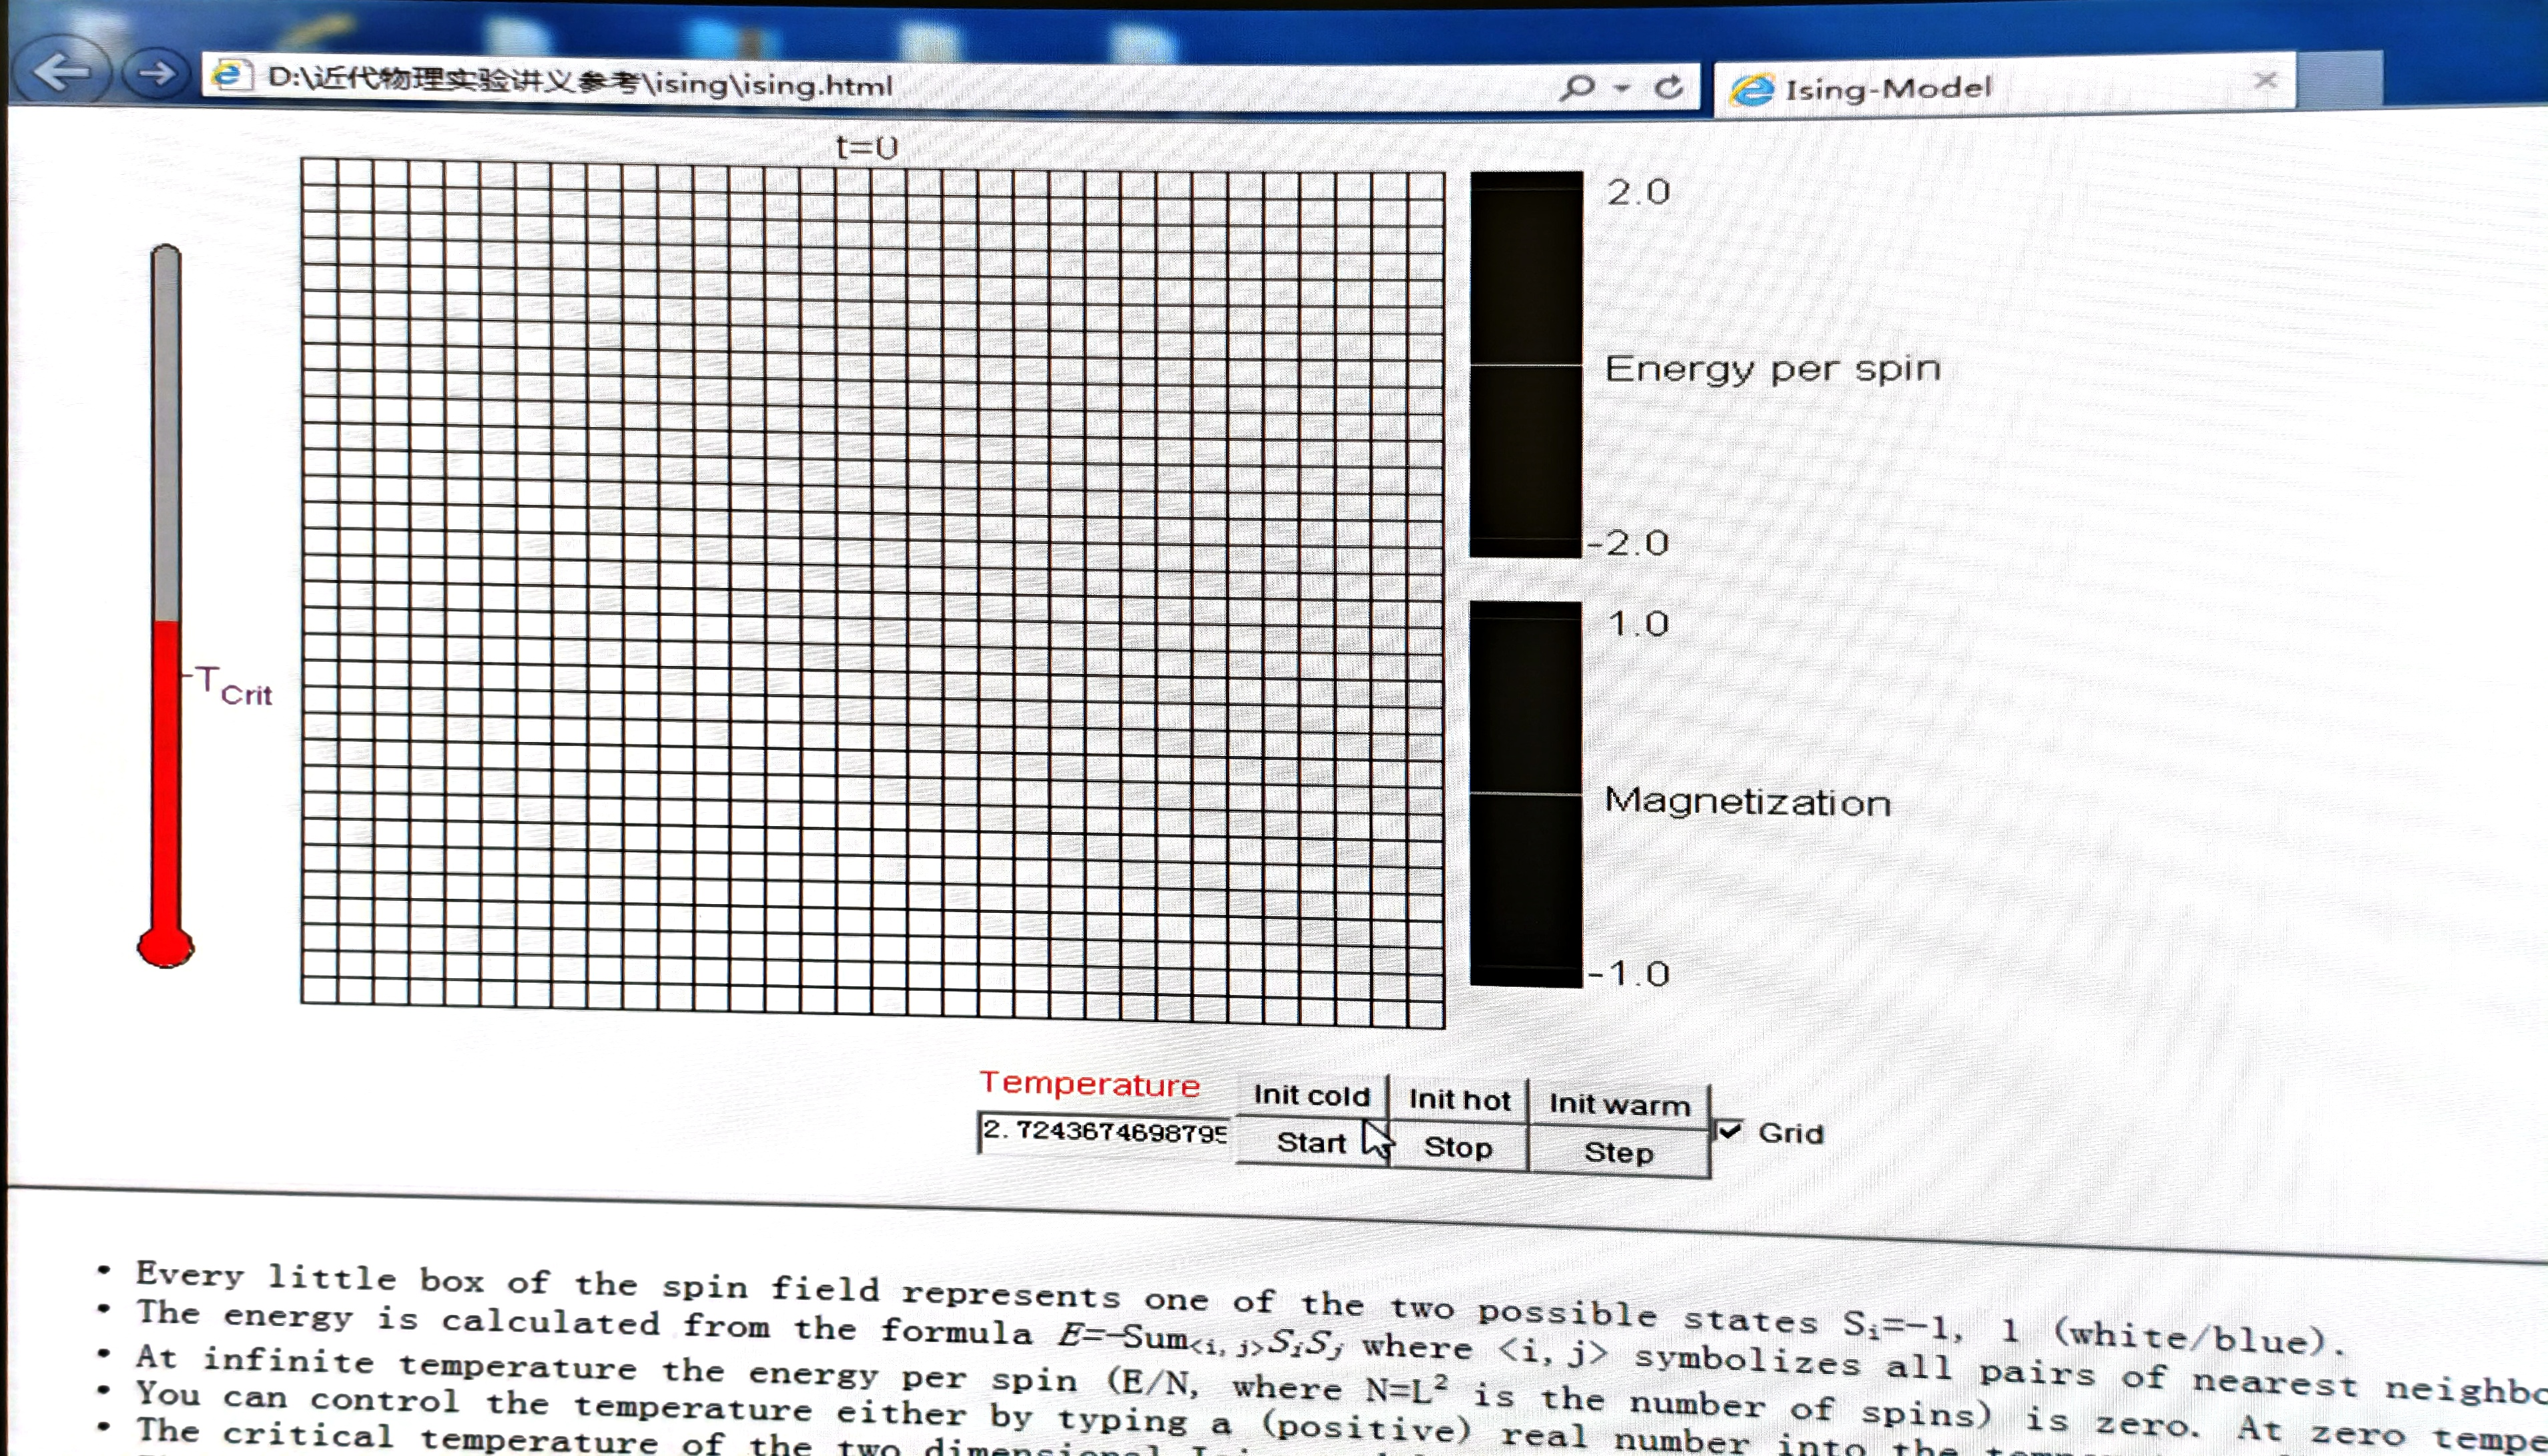
\includegraphics[width=\textwidth]{Figure/fig12.jpg}
        \caption{演化前期的孤立有序小岛}
    \end{subfigure}
    \hfill
    \begin{subfigure}[b]{0.32\textwidth}
        \centering
        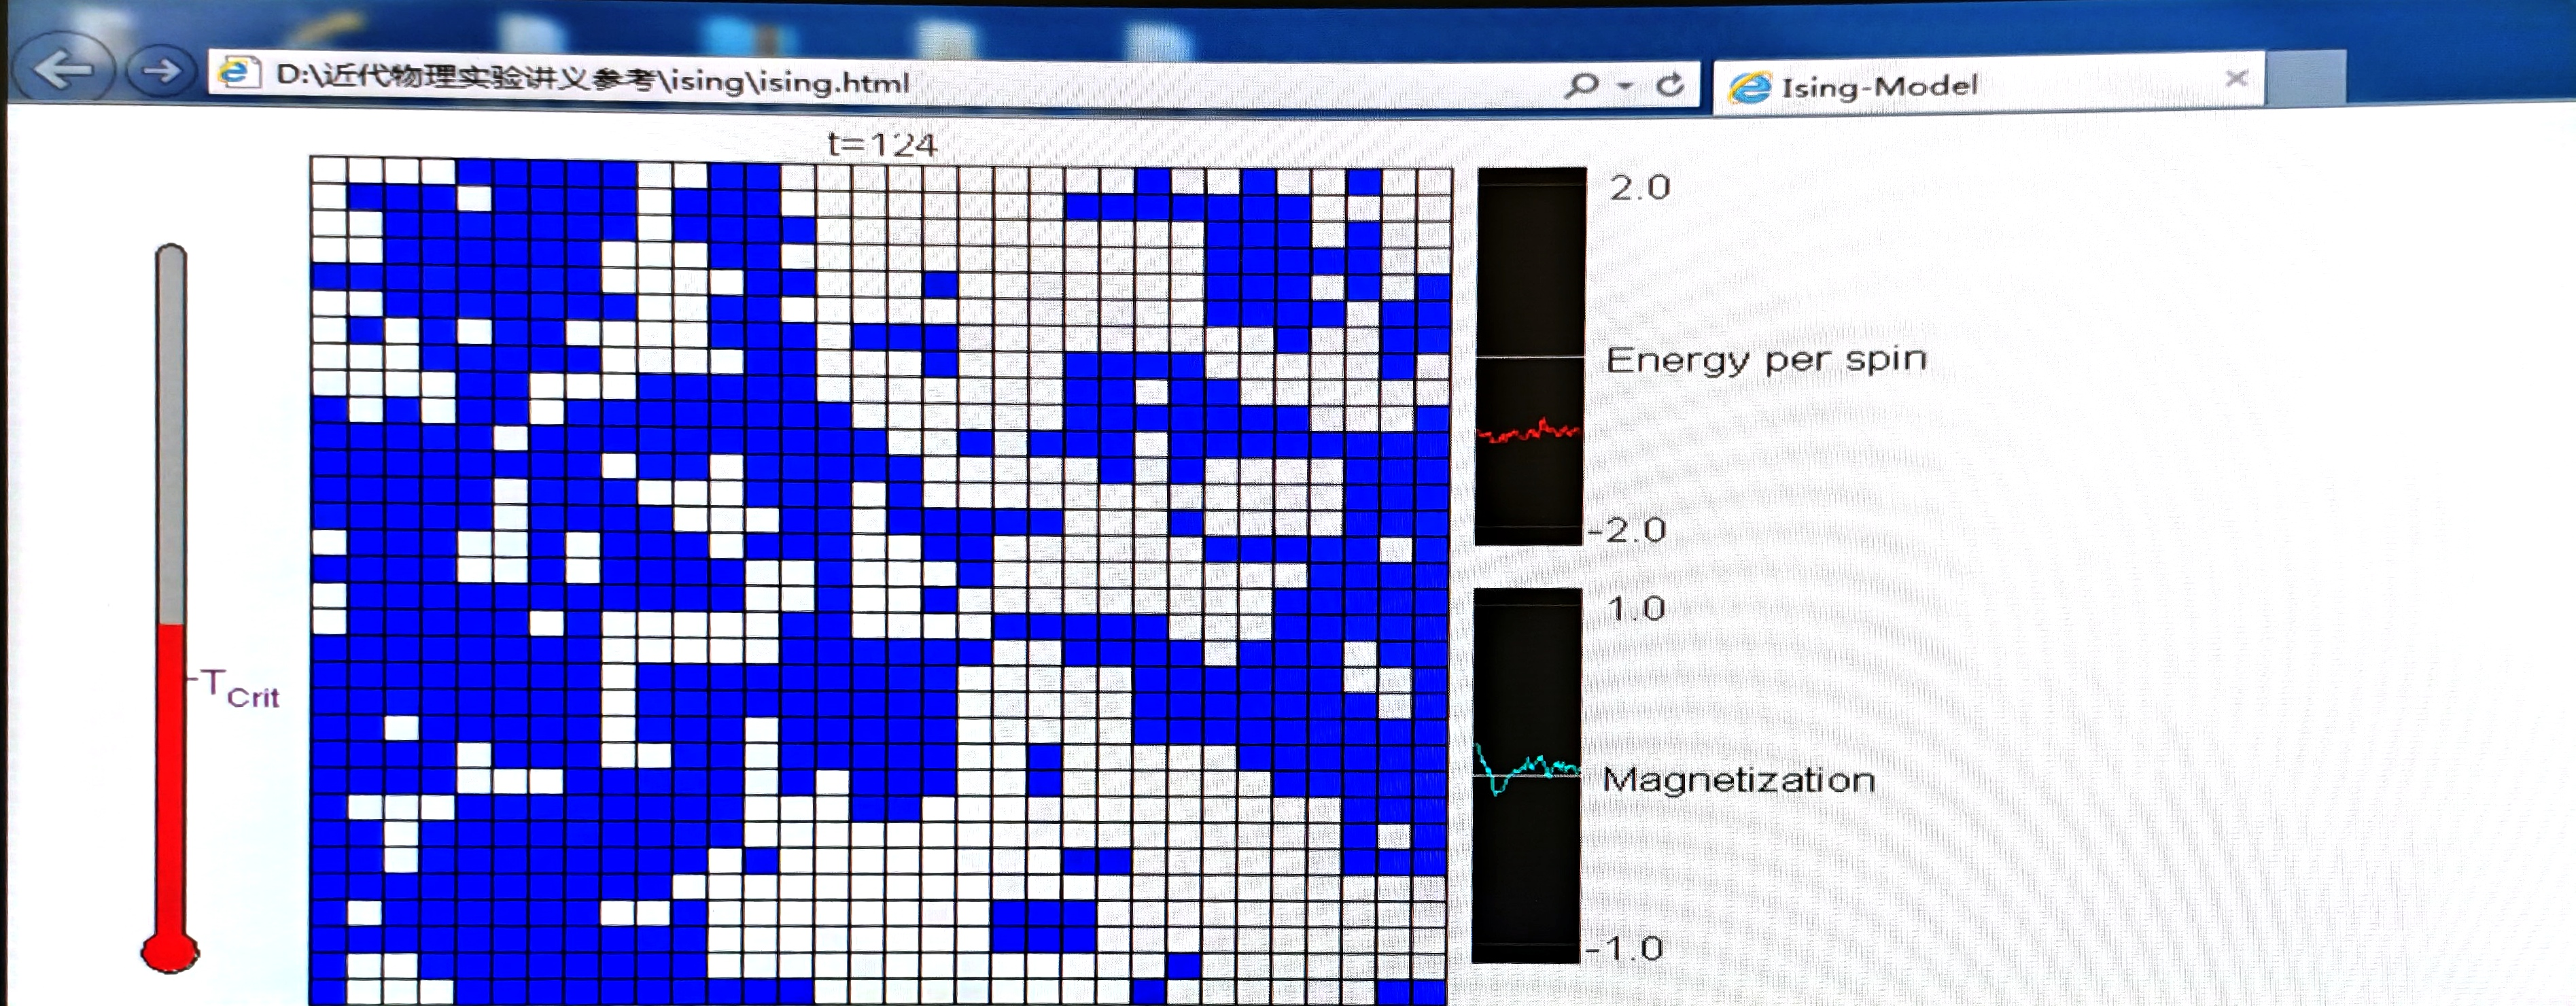
\includegraphics[width=\textwidth]{Figure/fig13.jpg}
        \caption{有序自旋畴扩张吞并阶段}
    \end{subfigure}
    \hfill
    \begin{subfigure}[b]{0.32\textwidth}
        \centering
        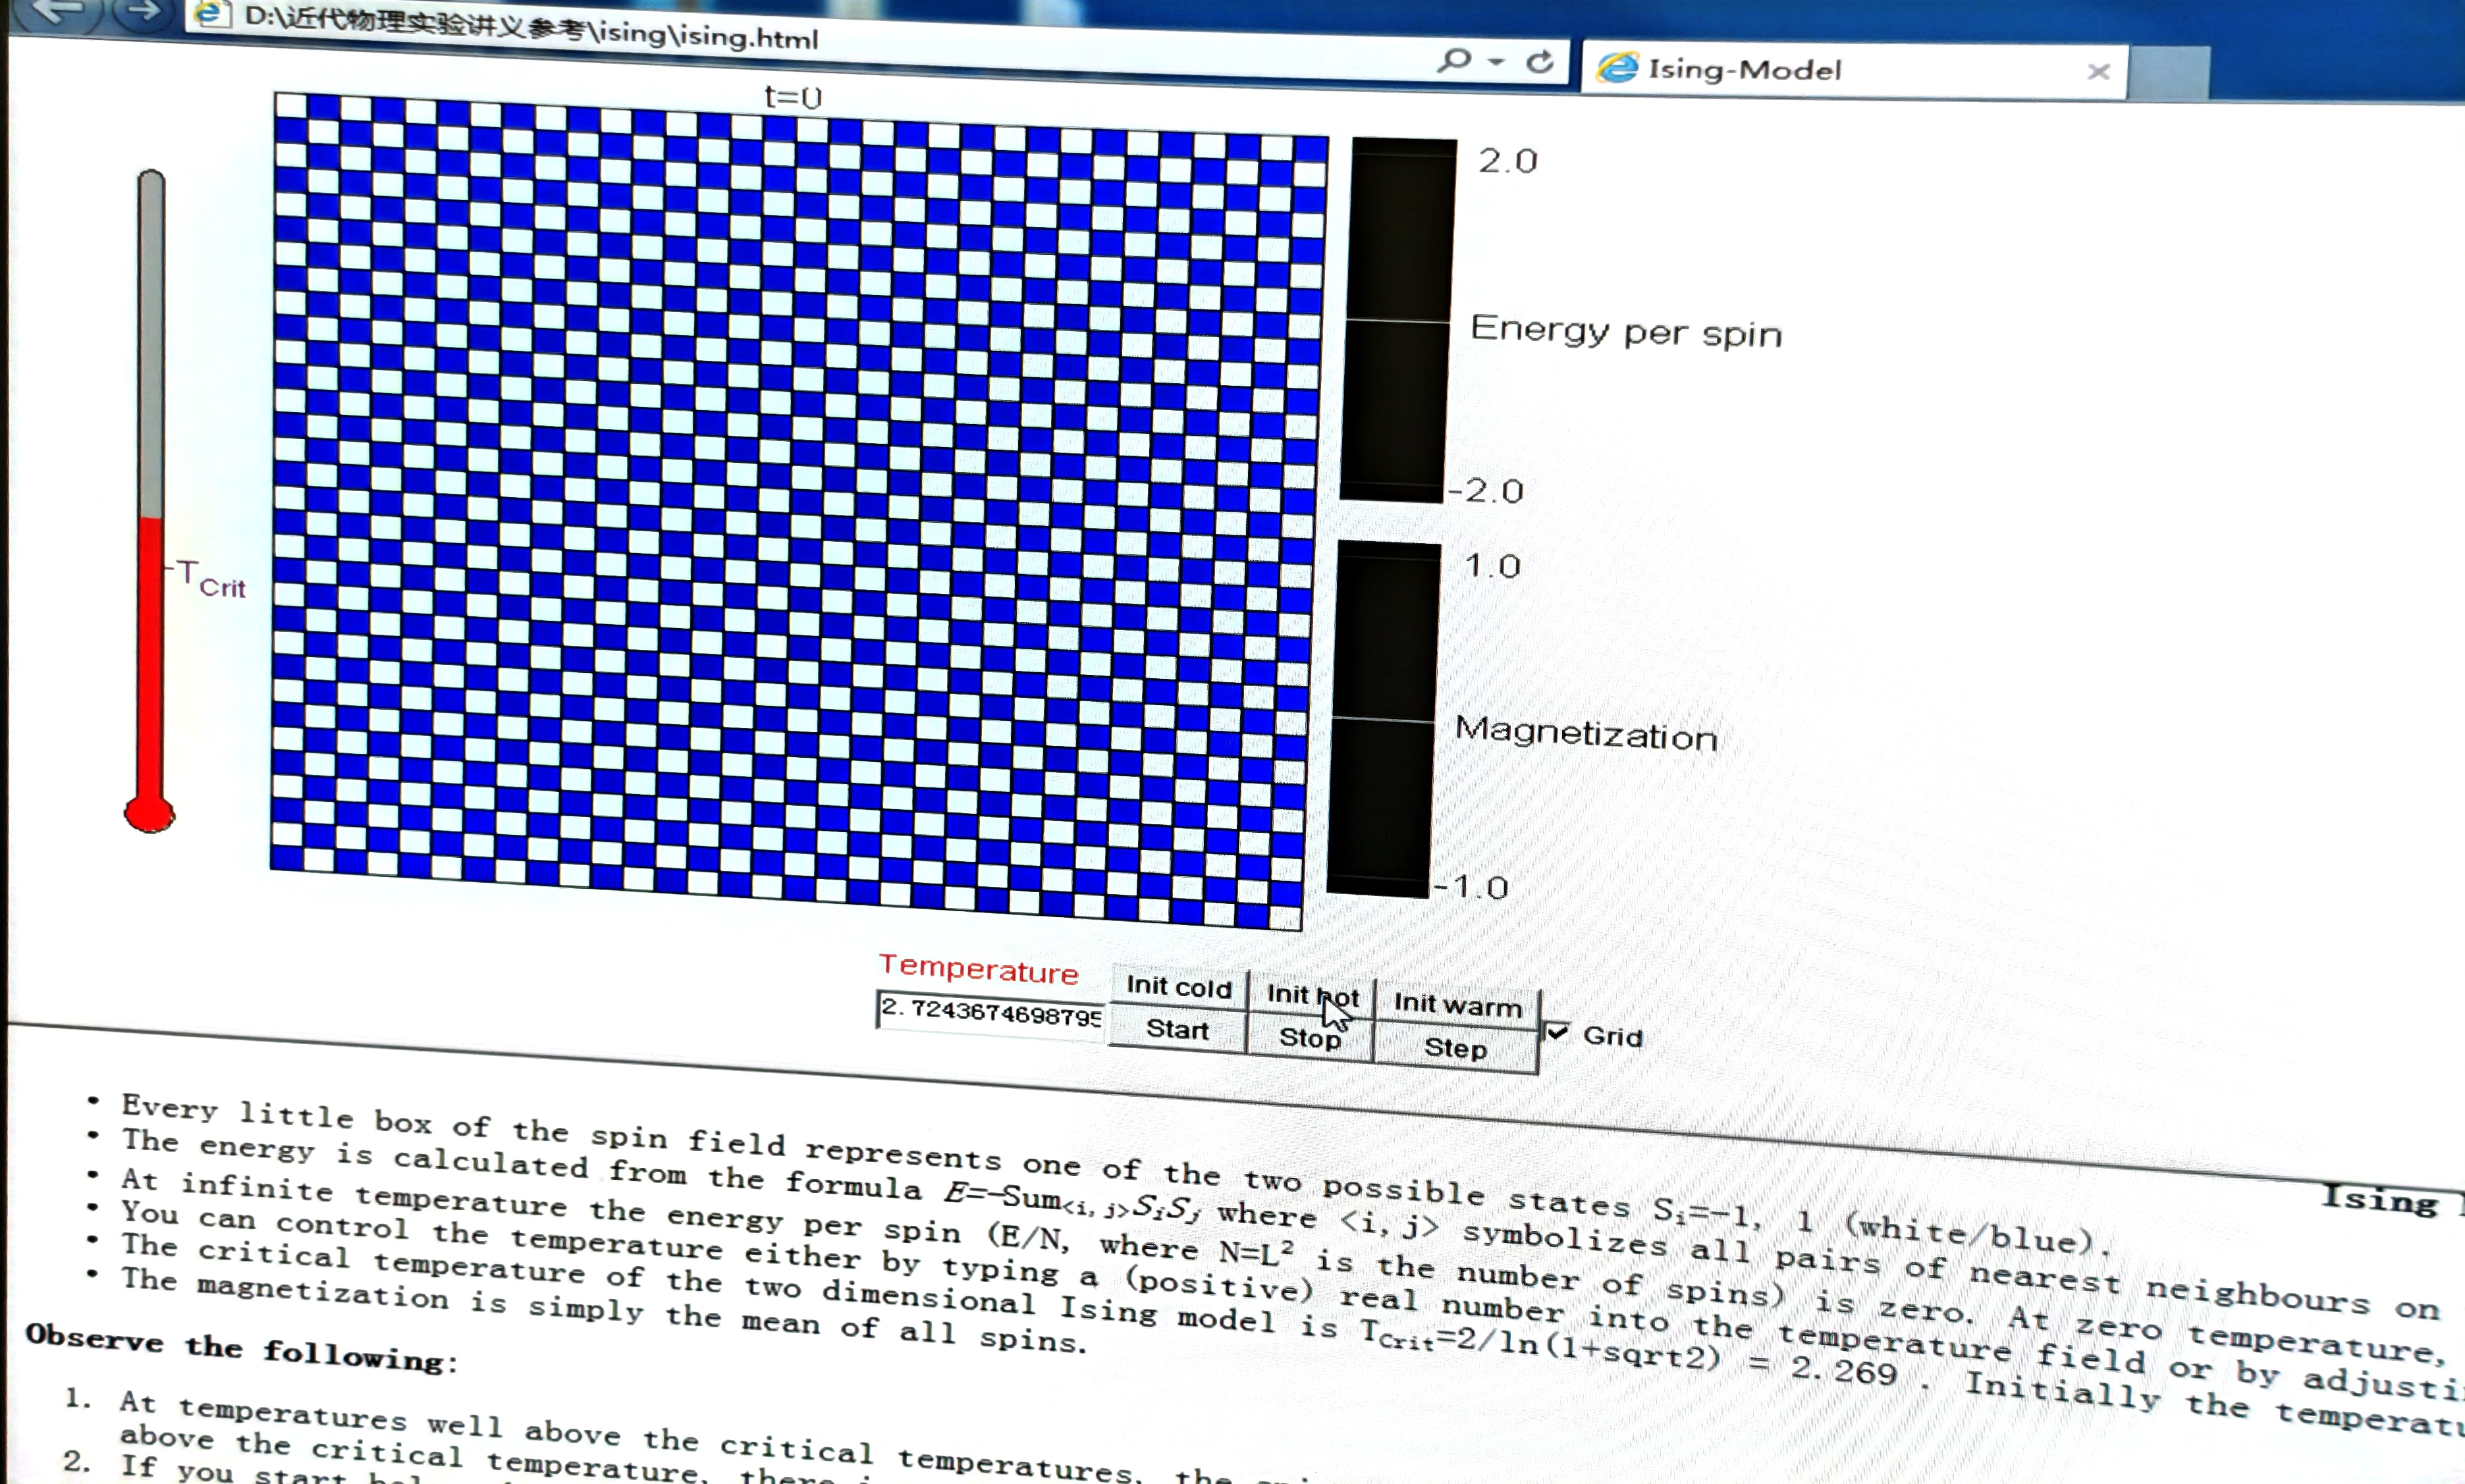
\includegraphics[width=\textwidth]{Figure/fig14.jpg}
        \caption{几乎完全自发磁化状态}
    \end{subfigure}
    \caption{低温有序相（$T < T_c$）自旋凝聚过程及强自发磁化现象实时截图}
    \label{fig:low_temp_evolve}
\end{figure}

\subsection{系统热力学平衡过程的监测}
图 \ref{fig:relaxation_process} 展示了平均内能、平均磁化强度以及能量/自选涨落随模拟步数（MCS）的演化曲线。可以看出，经过约 500-1000 步的弛豫步，系统已经完全偏离初始设置，平稳在当前温度下的热平衡涨落中心。
\begin{figure}[H]
    \centering
    \begin{subfigure}[b]{0.32\textwidth}
        \centering
        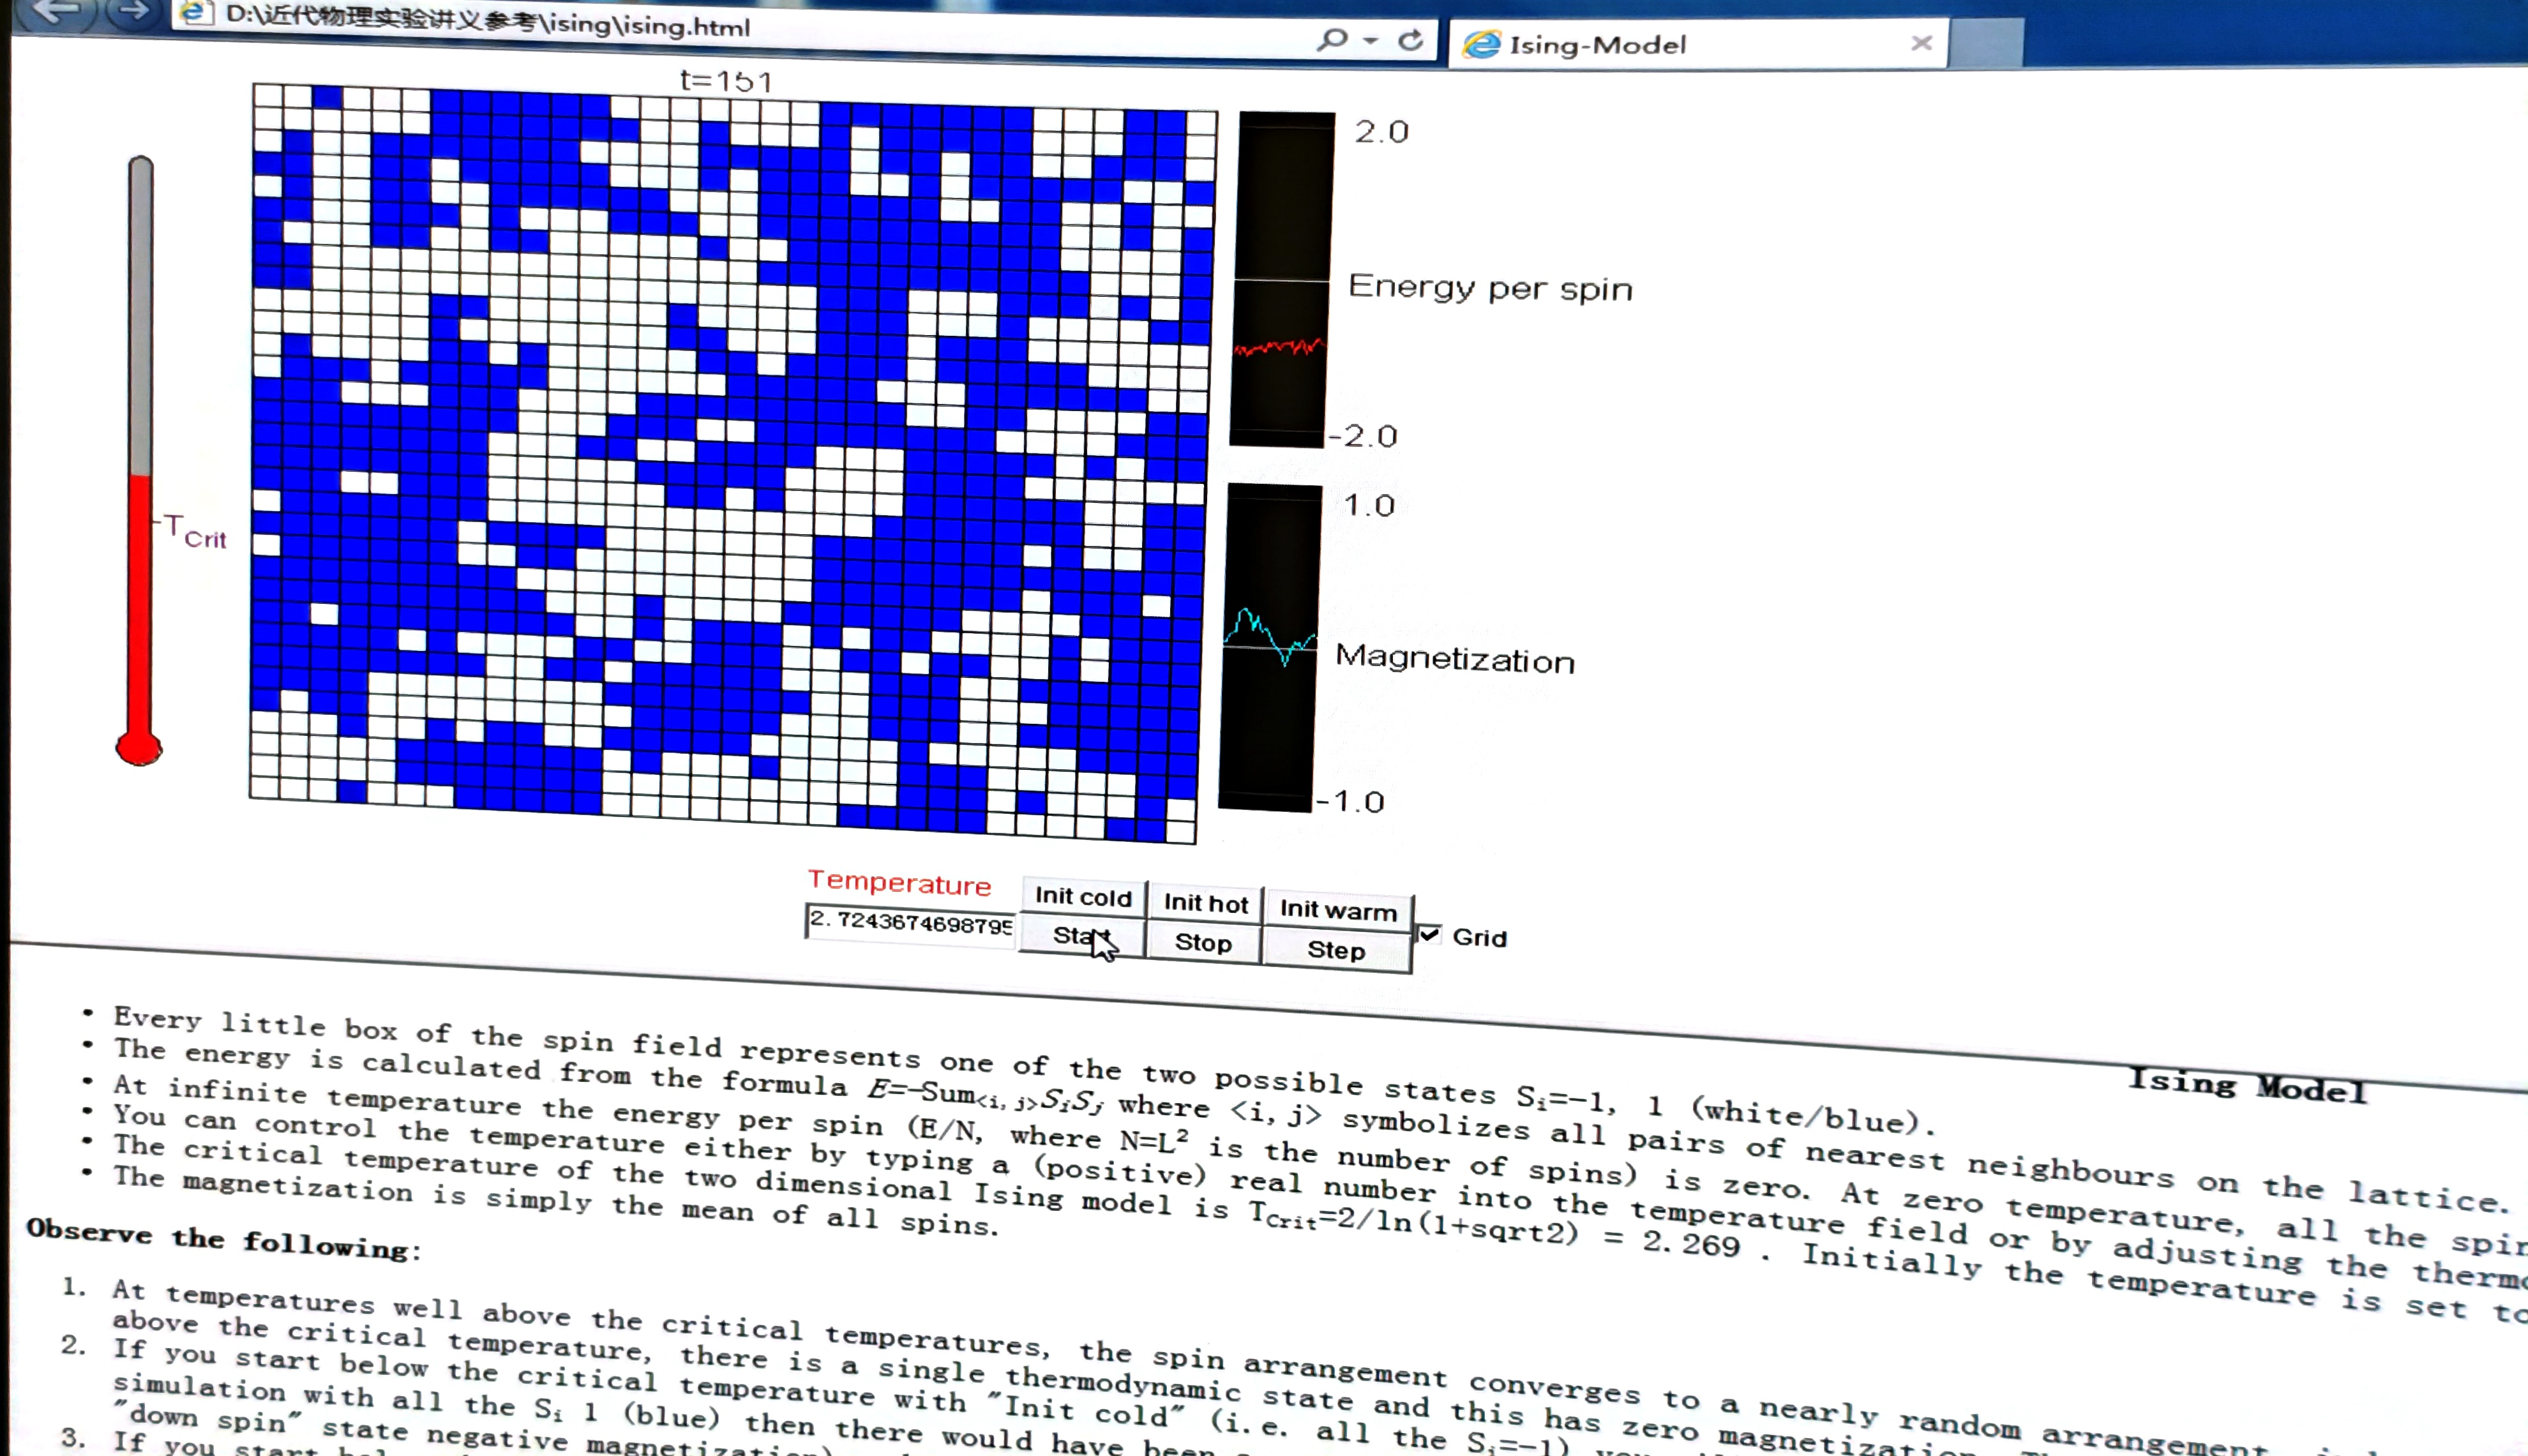
\includegraphics[width=\textwidth]{Figure/fig15.jpg}
        \caption{内能随MCS的弛豫收敛曲线}
    \end{subfigure}
    \hfill
    \begin{subfigure}[b]{0.32\textwidth}
        \centering
        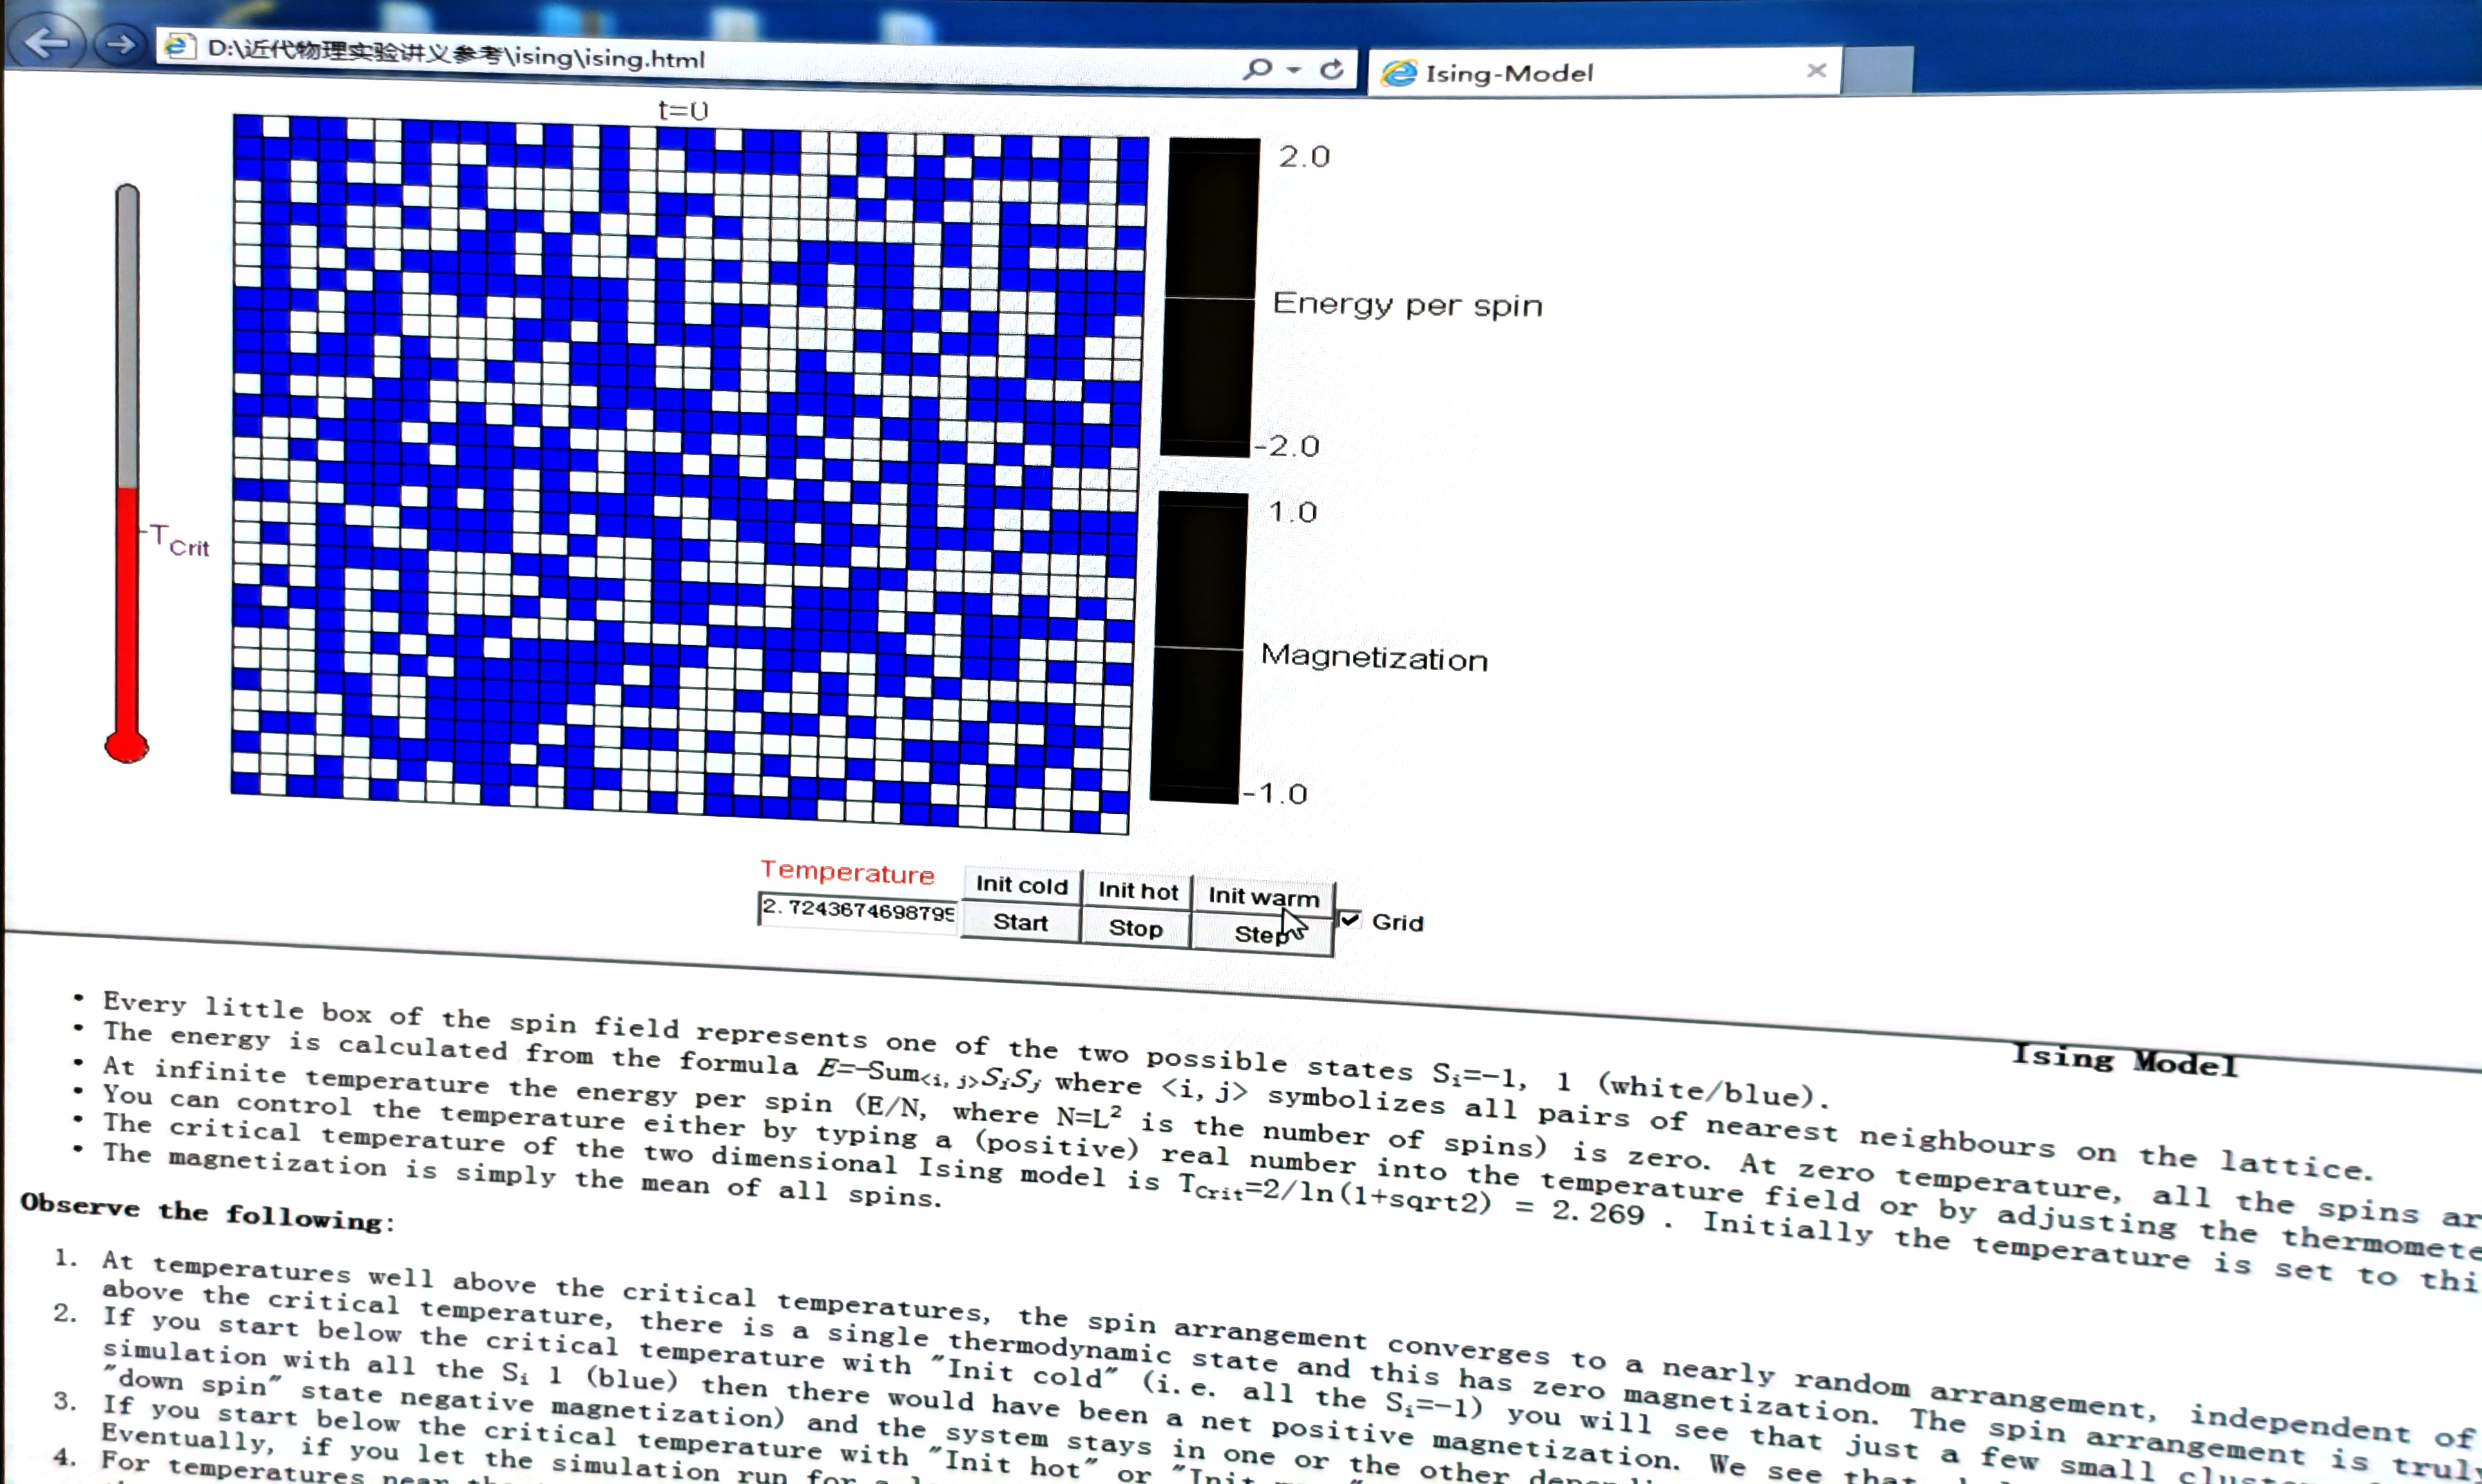
\includegraphics[width=\textwidth]{Figure/fig16.jpg}
        \caption{磁化强度随MCS的弛豫收敛曲线}
    \end{subfigure}
    \hfill
    \begin{subfigure}[b]{0.32\textwidth}
        \centering
        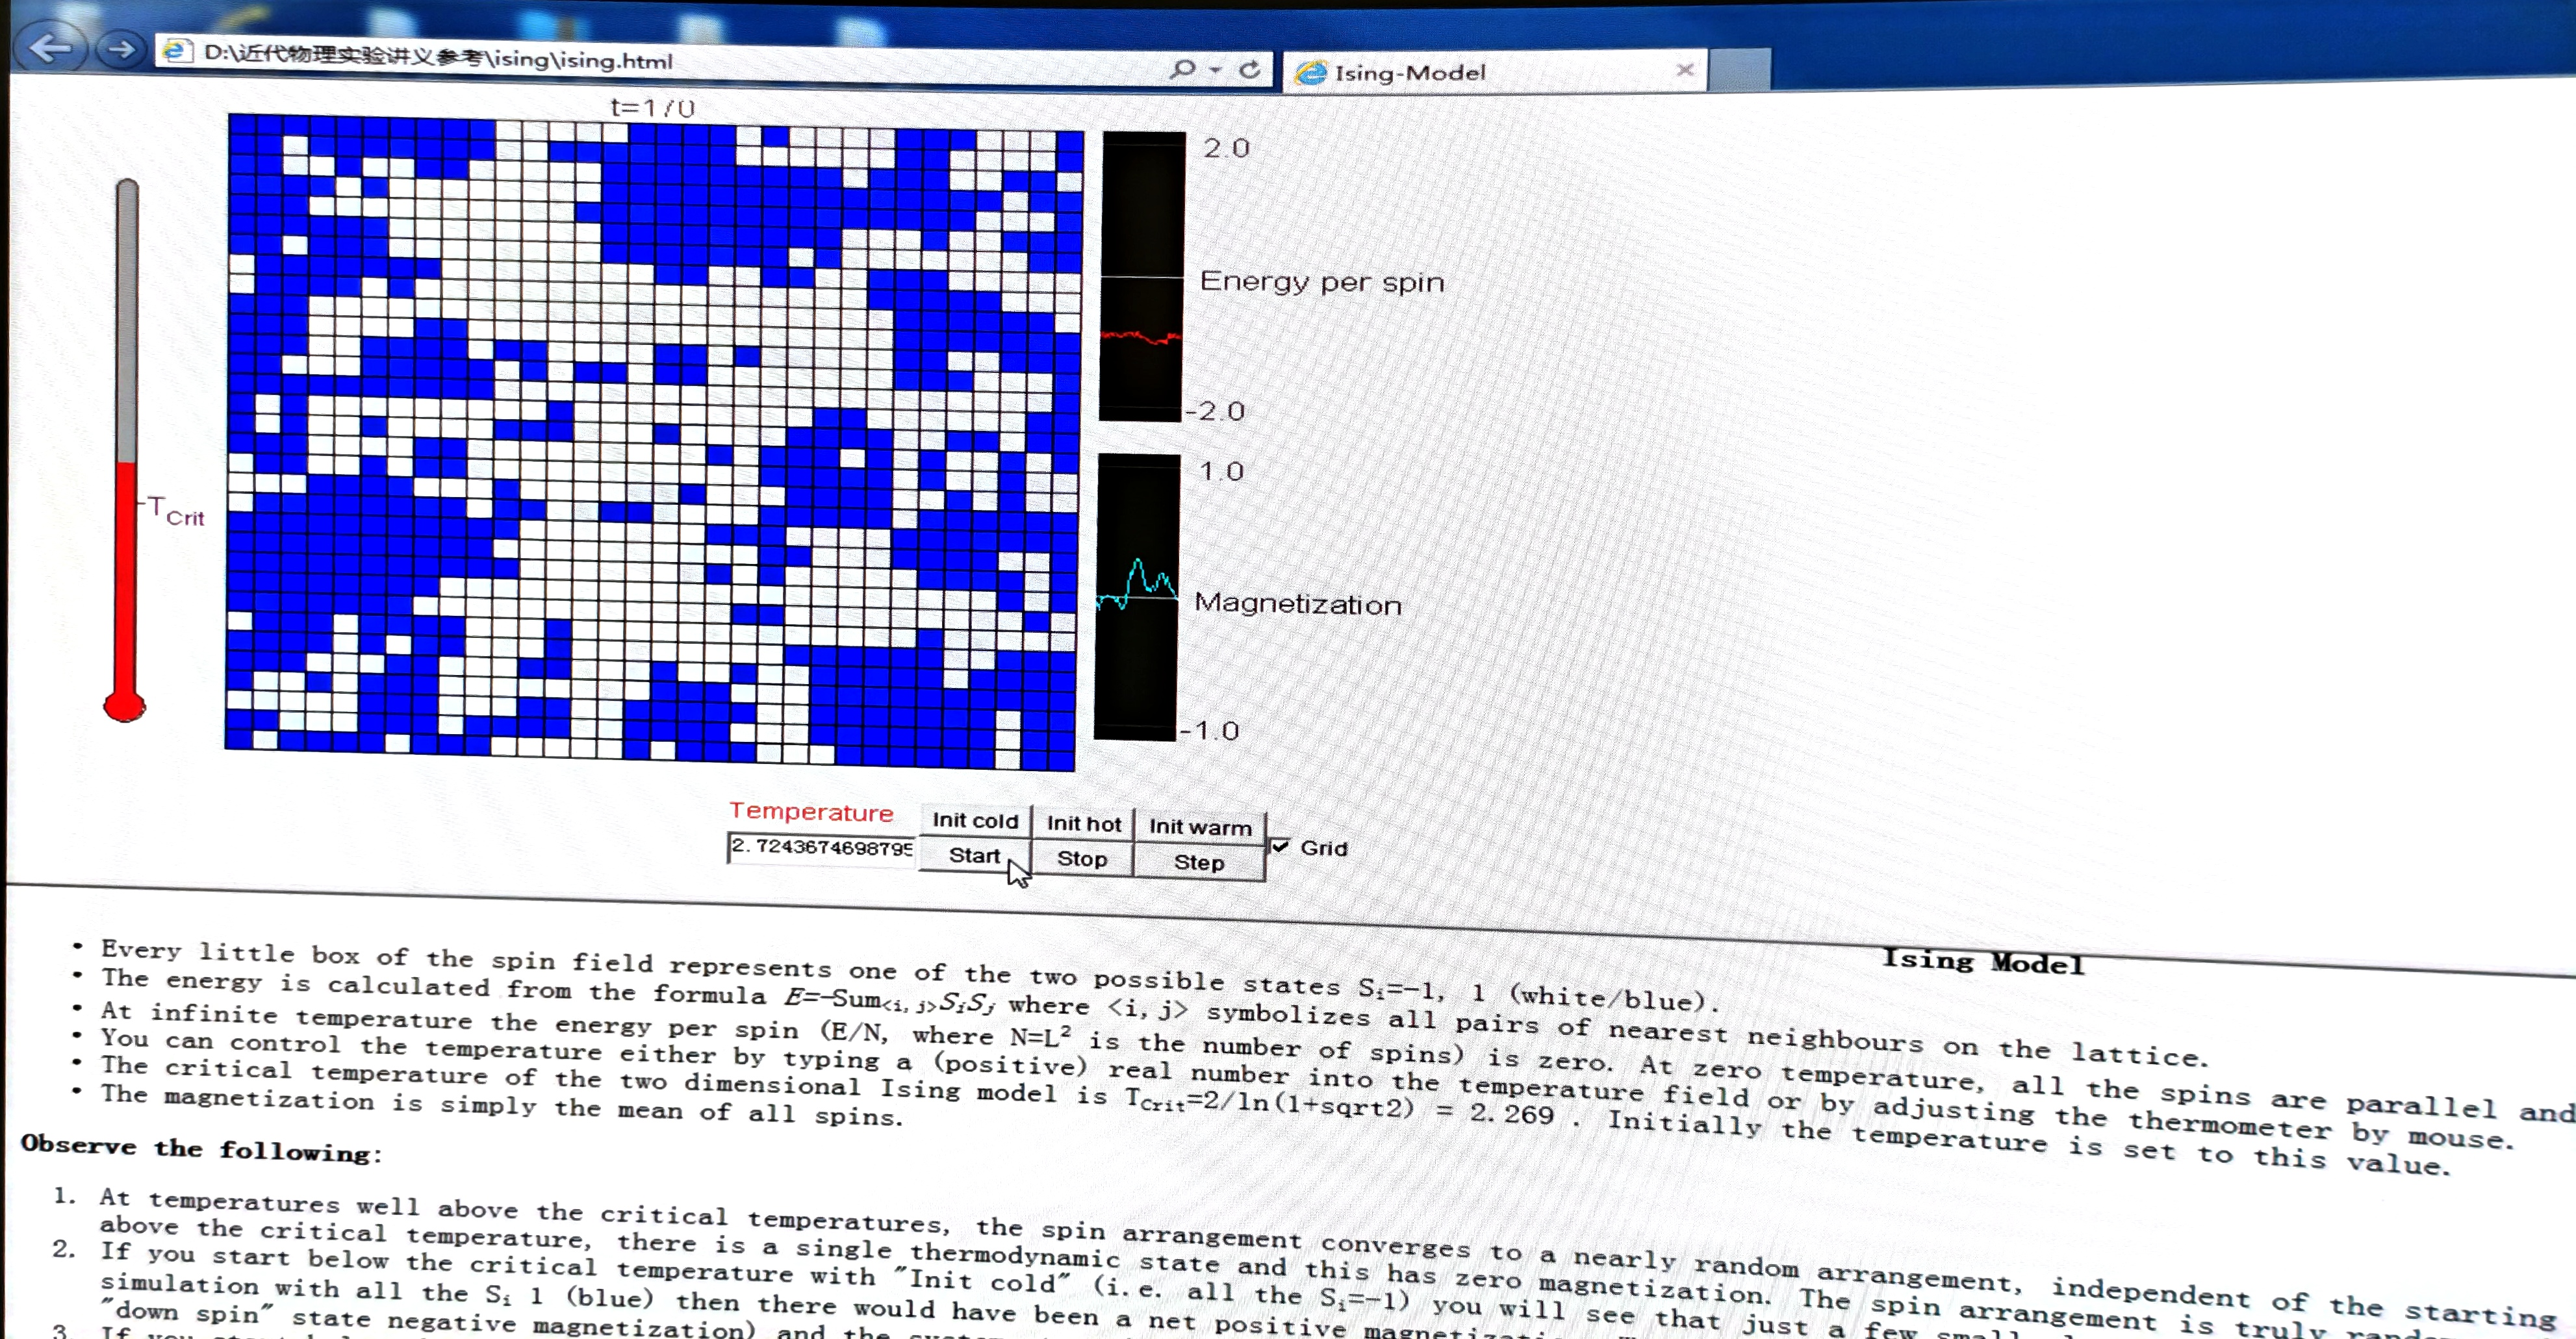
\includegraphics[width=\textwidth]{Figure/fig17.jpg}
        \caption{高频热涨落的平衡曲线}
    \end{subfigure}
    \caption{热力学物理量弛豫到平衡态过程的动态监视曲线图}
    \label{fig:relaxation_process}
\end{figure}

\subsection{平均内能与磁化强度随温度的变化分析}
图 \ref{fig:e_m_vs_temp} 展示了二维 Ising 模型中平均内能 $E$ 和平均自旋磁化强度 $|m|$ 随温度 $T$ 的统计曲线。
\begin{figure}[H]
    \centering
    \begin{subfigure}[b]{0.32\textwidth}
        \centering
        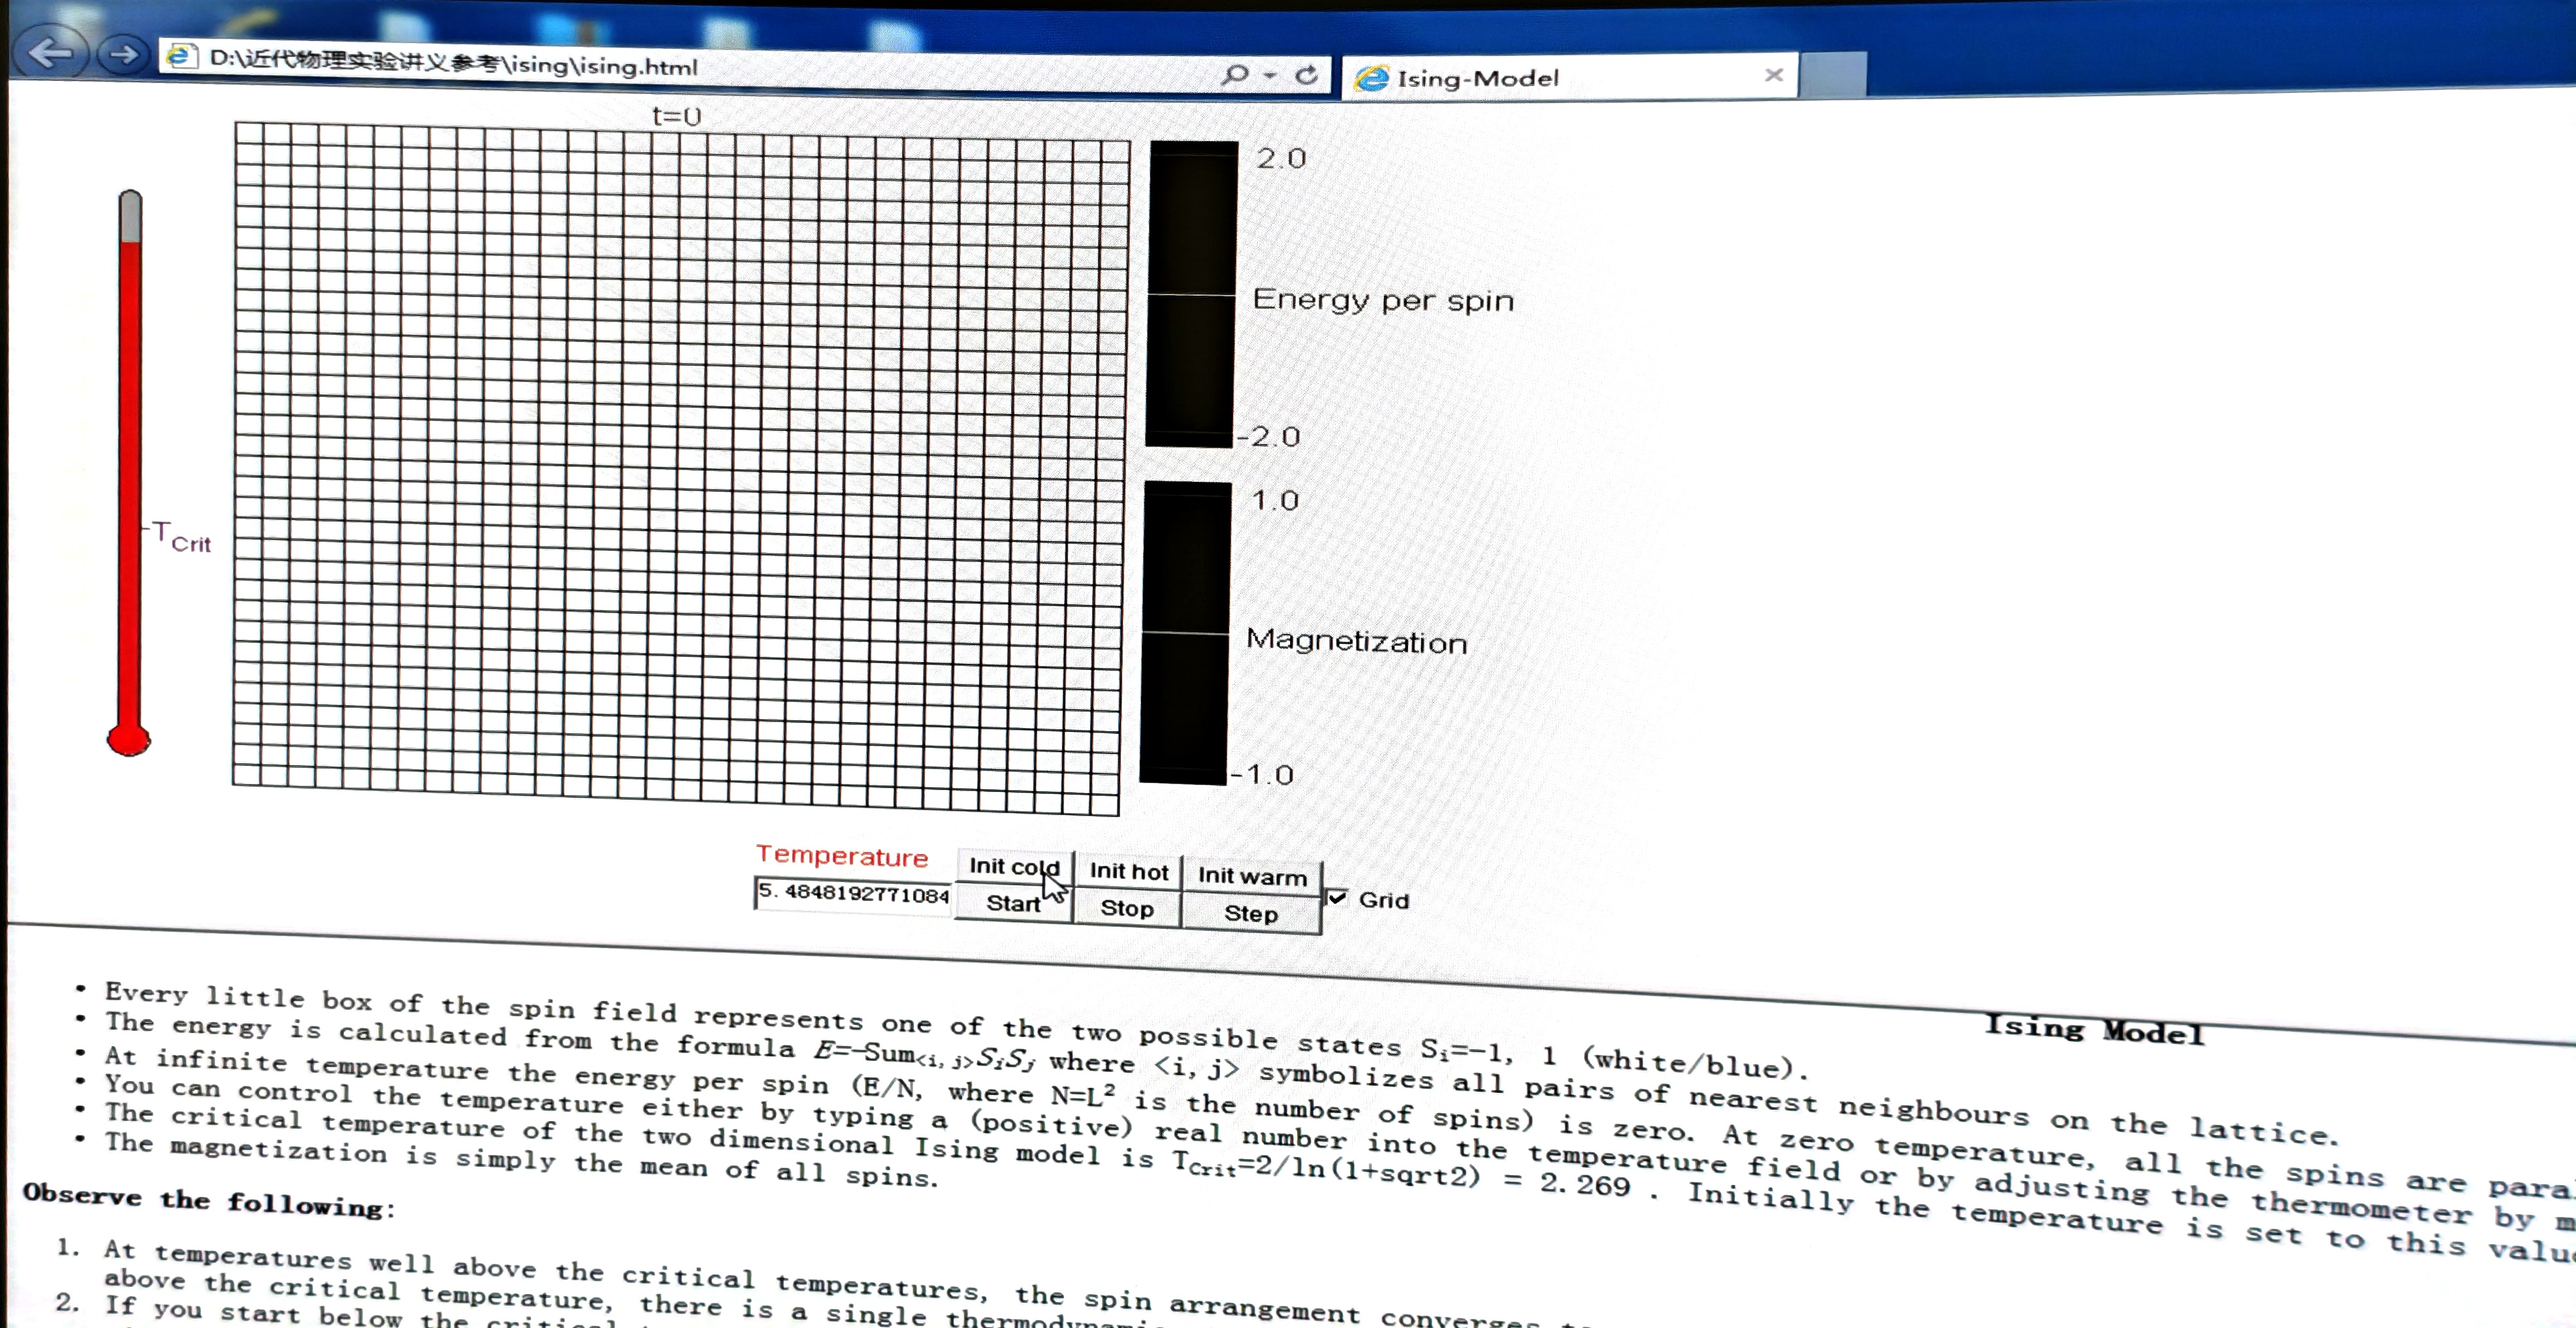
\includegraphics[width=\textwidth]{Figure/fig18.jpg}
        \caption{格点 $L=16$ 时的 $E$-$T$ 与 $M$-$T$ 曲线}
    \end{subfigure}
    \hfill
    \begin{subfigure}[b]{0.32\textwidth}
        \centering
        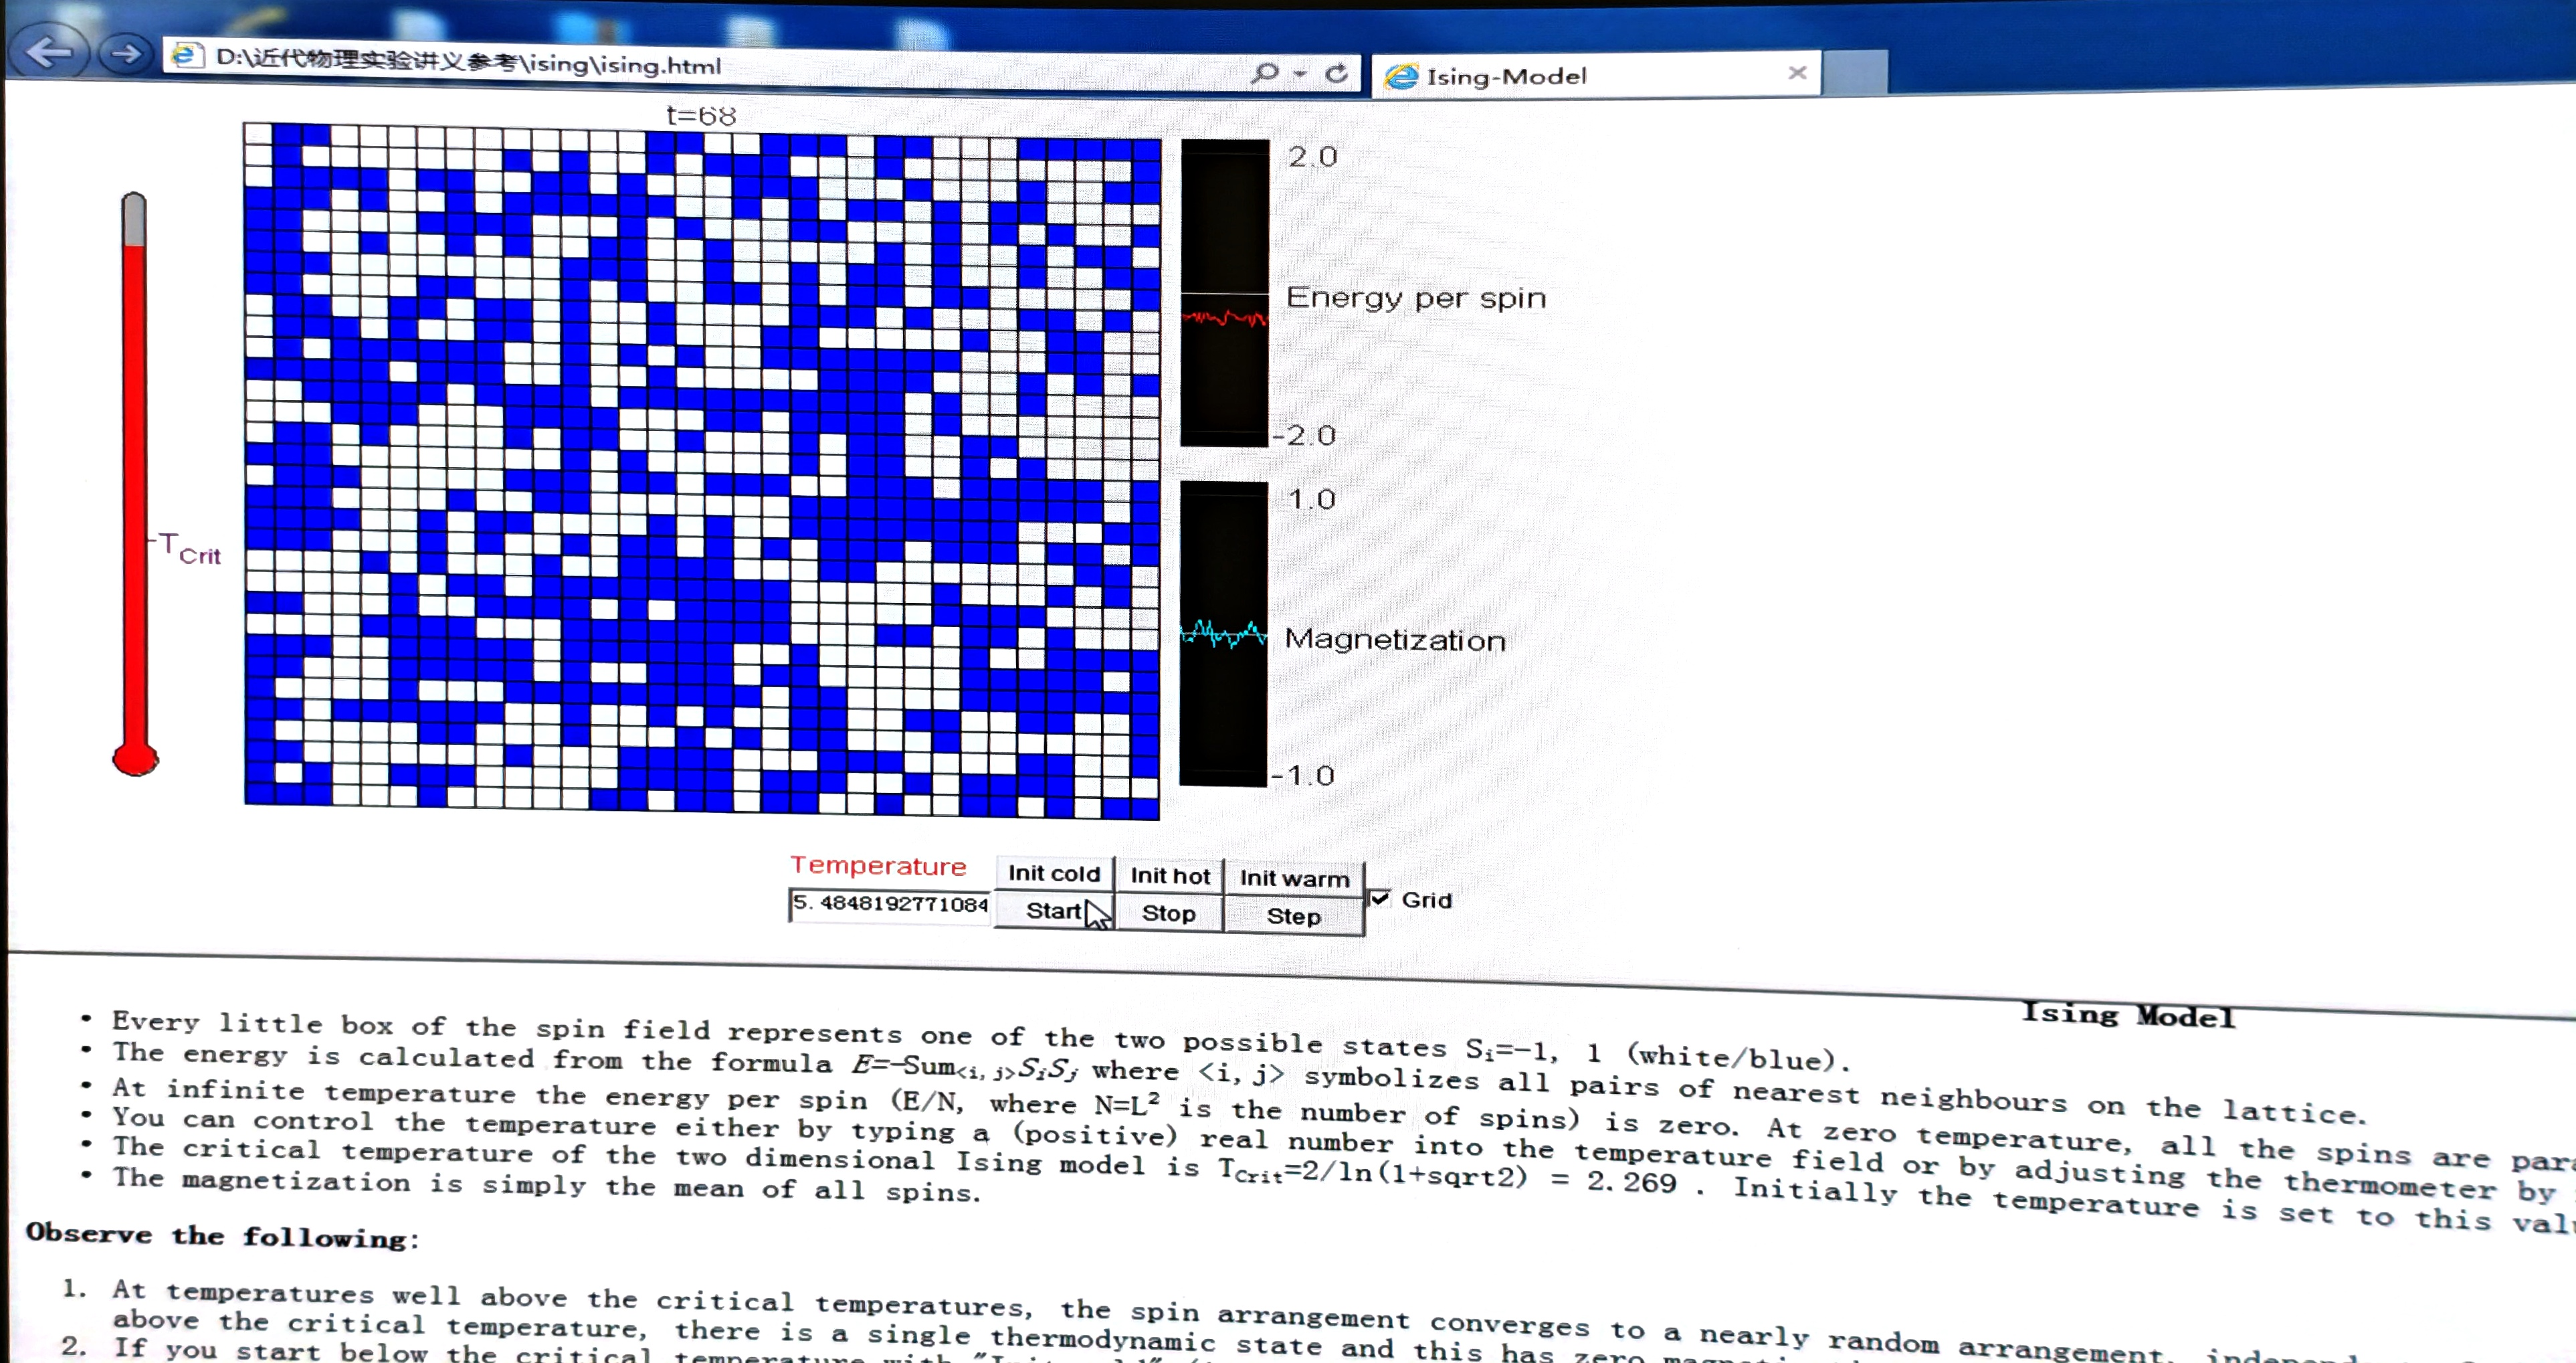
\includegraphics[width=\textwidth]{Figure/fig19.jpg}
        \caption{格点 $L=32$ 时的 $E$-$T$ 与 $M$-$T$ 曲线}
    \end{subfigure}
    \hfill
    \begin{subfigure}[b]{0.32\textwidth}
        \centering
        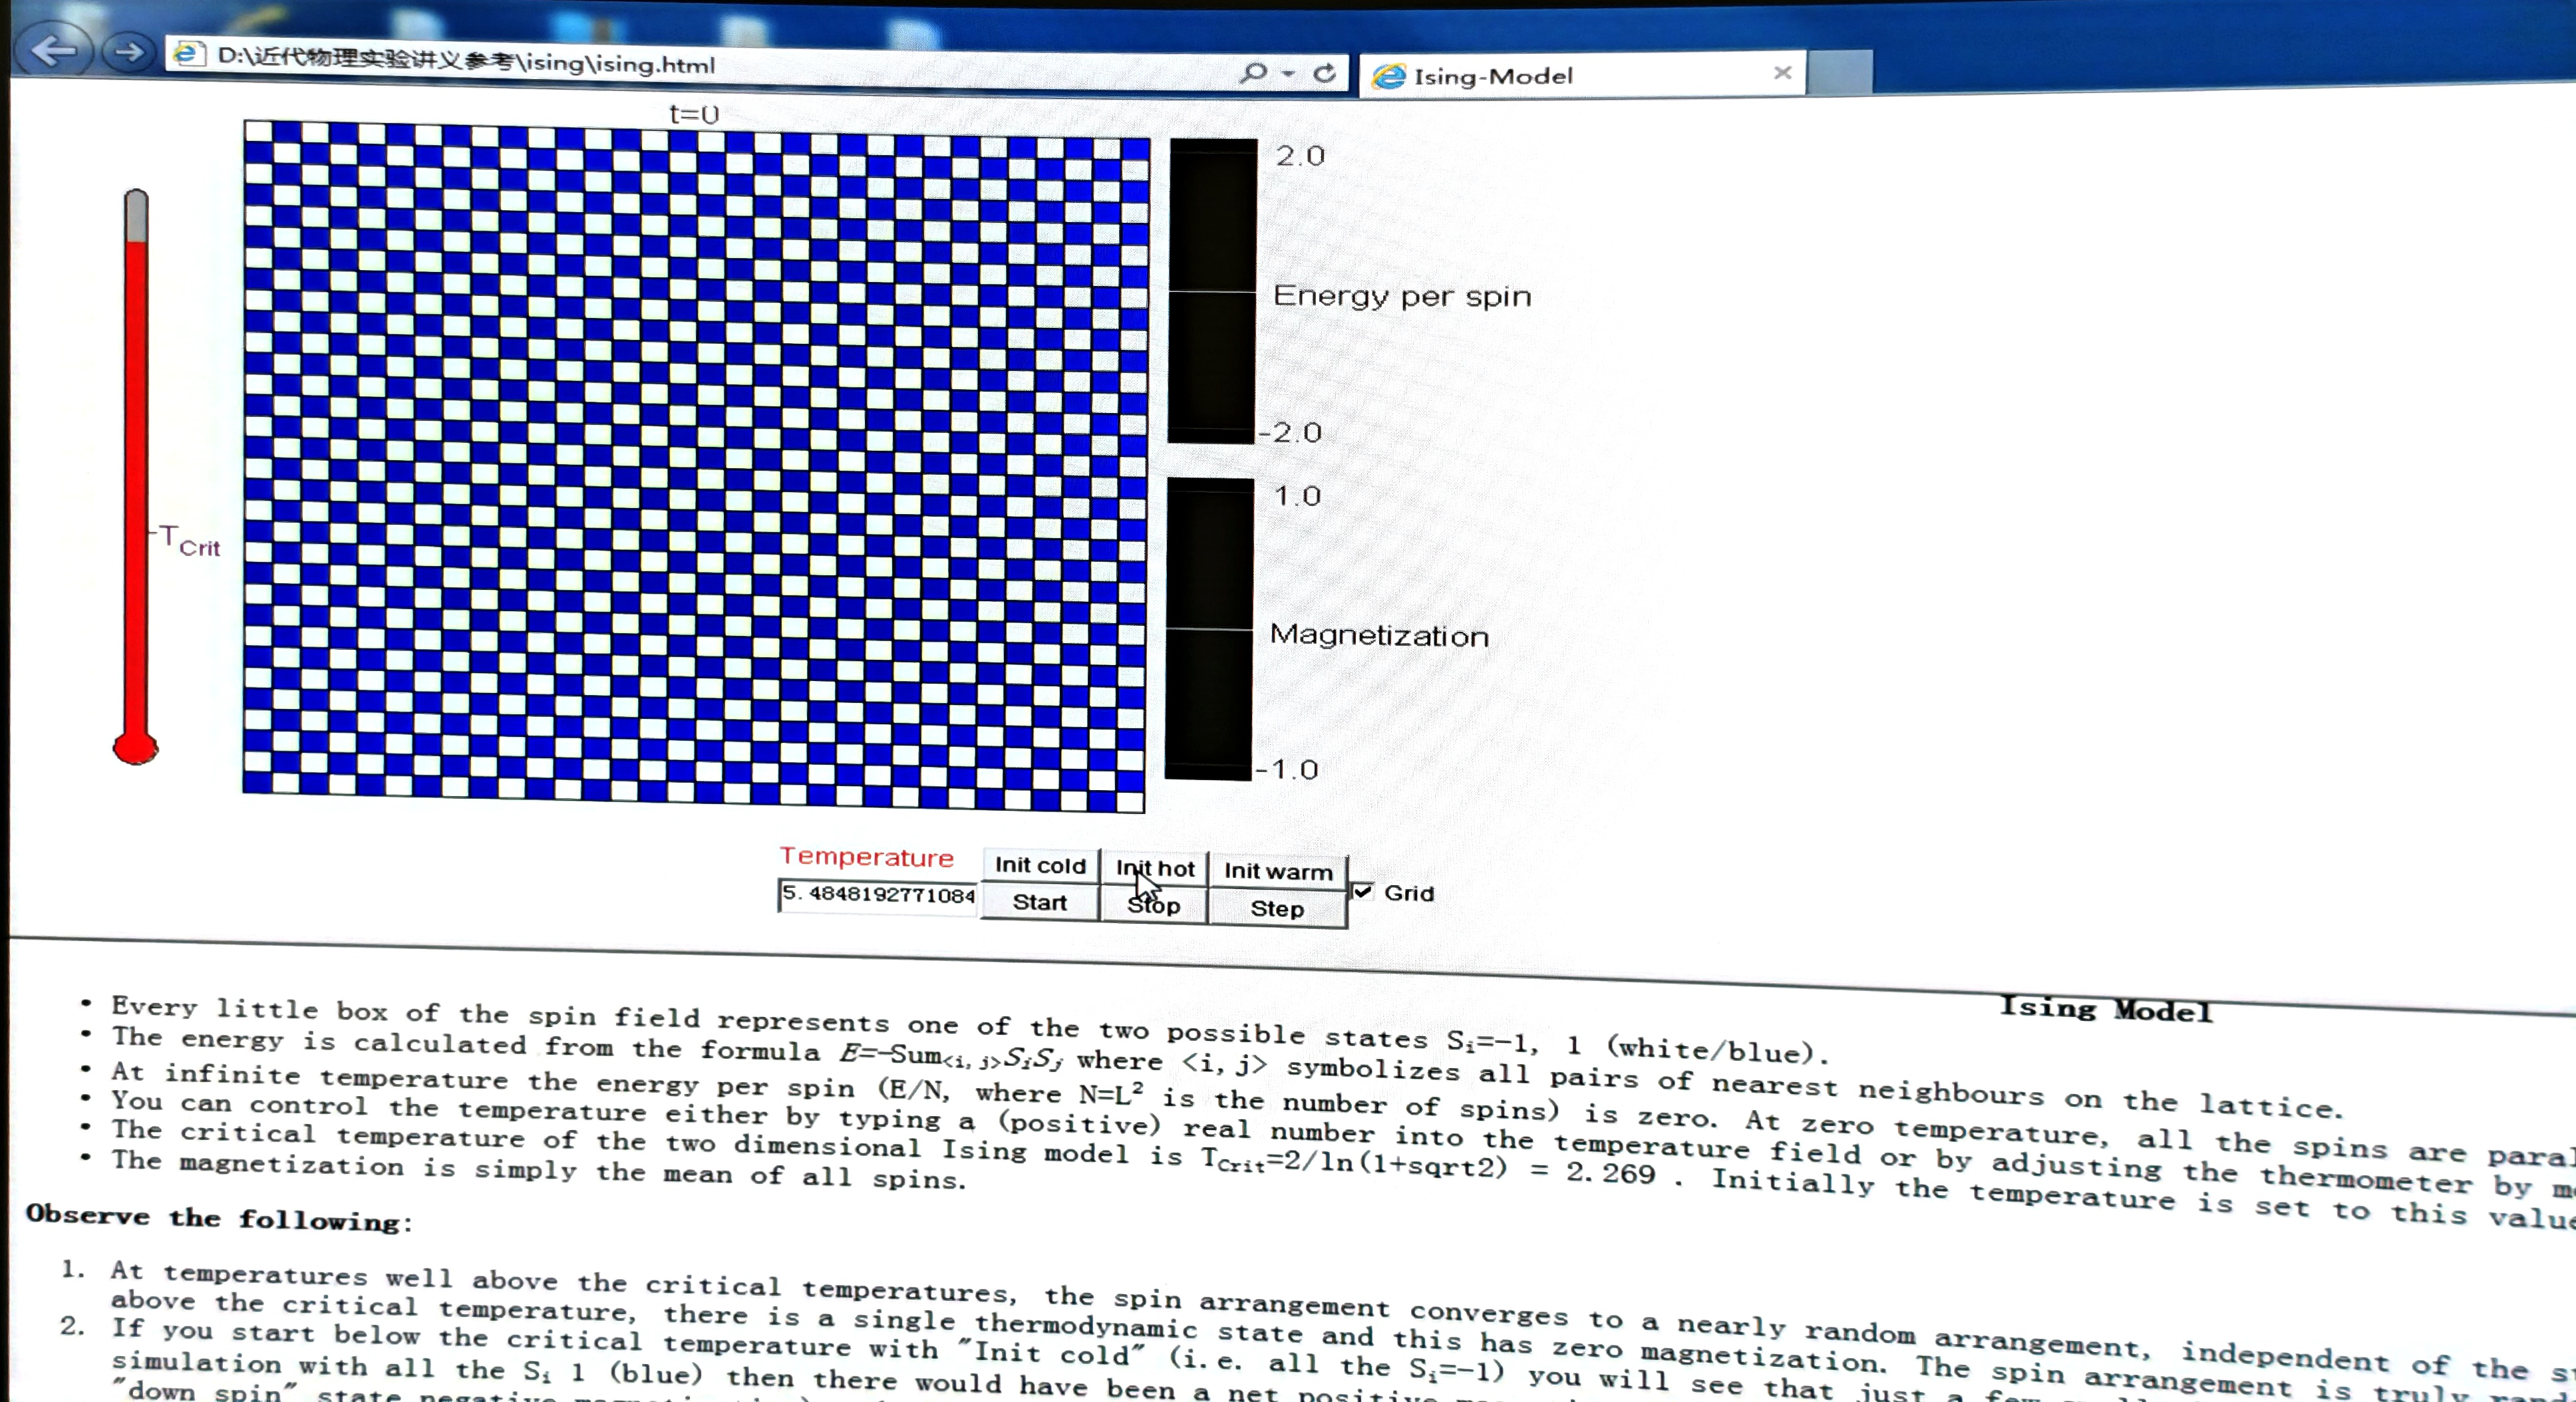
\includegraphics[width=\textwidth]{Figure/fig20.jpg}
        \caption{格点 $L=64$ 时的系统响应变化曲线}
    \end{subfigure}
    \caption{体系内能 $E$ 及自发磁化强度 $|m|$ 随温度 $T$ 的平衡态曲线（展示了明确的相变拐点）}
    \label{fig:e_m_vs_temp}
\end{figure}

对图 \ref{fig:e_m_vs_temp} 的分析结论如下：
\begin{enumerate}
    \item \textbf{自发磁化与对称性破缺}：在低温下（$T < 2.27$），即使无外部磁场，磁化强度 $|m|$ 亦高度稳定在 $\approx 1.0$。这表明系统发生了局域自旋朝向相同方向排列的**对称性破缺**，展现铁磁性。当温度升高逼近临界点时，由于热运动剧烈，大块有序自旋畴破裂，磁化强度迅速崩溃。在 $T > 2.27$ 后，$|m|$ 降至趋于 0。这符合连续相变（二级相变）的典型特征。
    \item \textbf{内能曲线}：在 $T \to 0$ 时，平均能量每自旋逼近最小极限 $-2J$（每个自旋 4 个键，各分担一半能量）。当温度升高时内能单调上升。在临界温度附近，能量曲线斜率急剧增加，出现拐点（微商发散点），对应于相变时的剧烈内能涨落。
\end{enumerate}

\subsection{比热与磁化率随温度的涨落发散分析}
图 \ref{fig:cv_chi_vs_temp} 记录了系统利用起伏公式（能量和磁化强度的涨落）算得的系统比热 $C_v$ 及磁化率 $\chi$随温度 $T$ 的响应变化曲线。
\begin{figure}[H]
    \centering
    \begin{subfigure}[b]{0.32\textwidth}
        \centering
        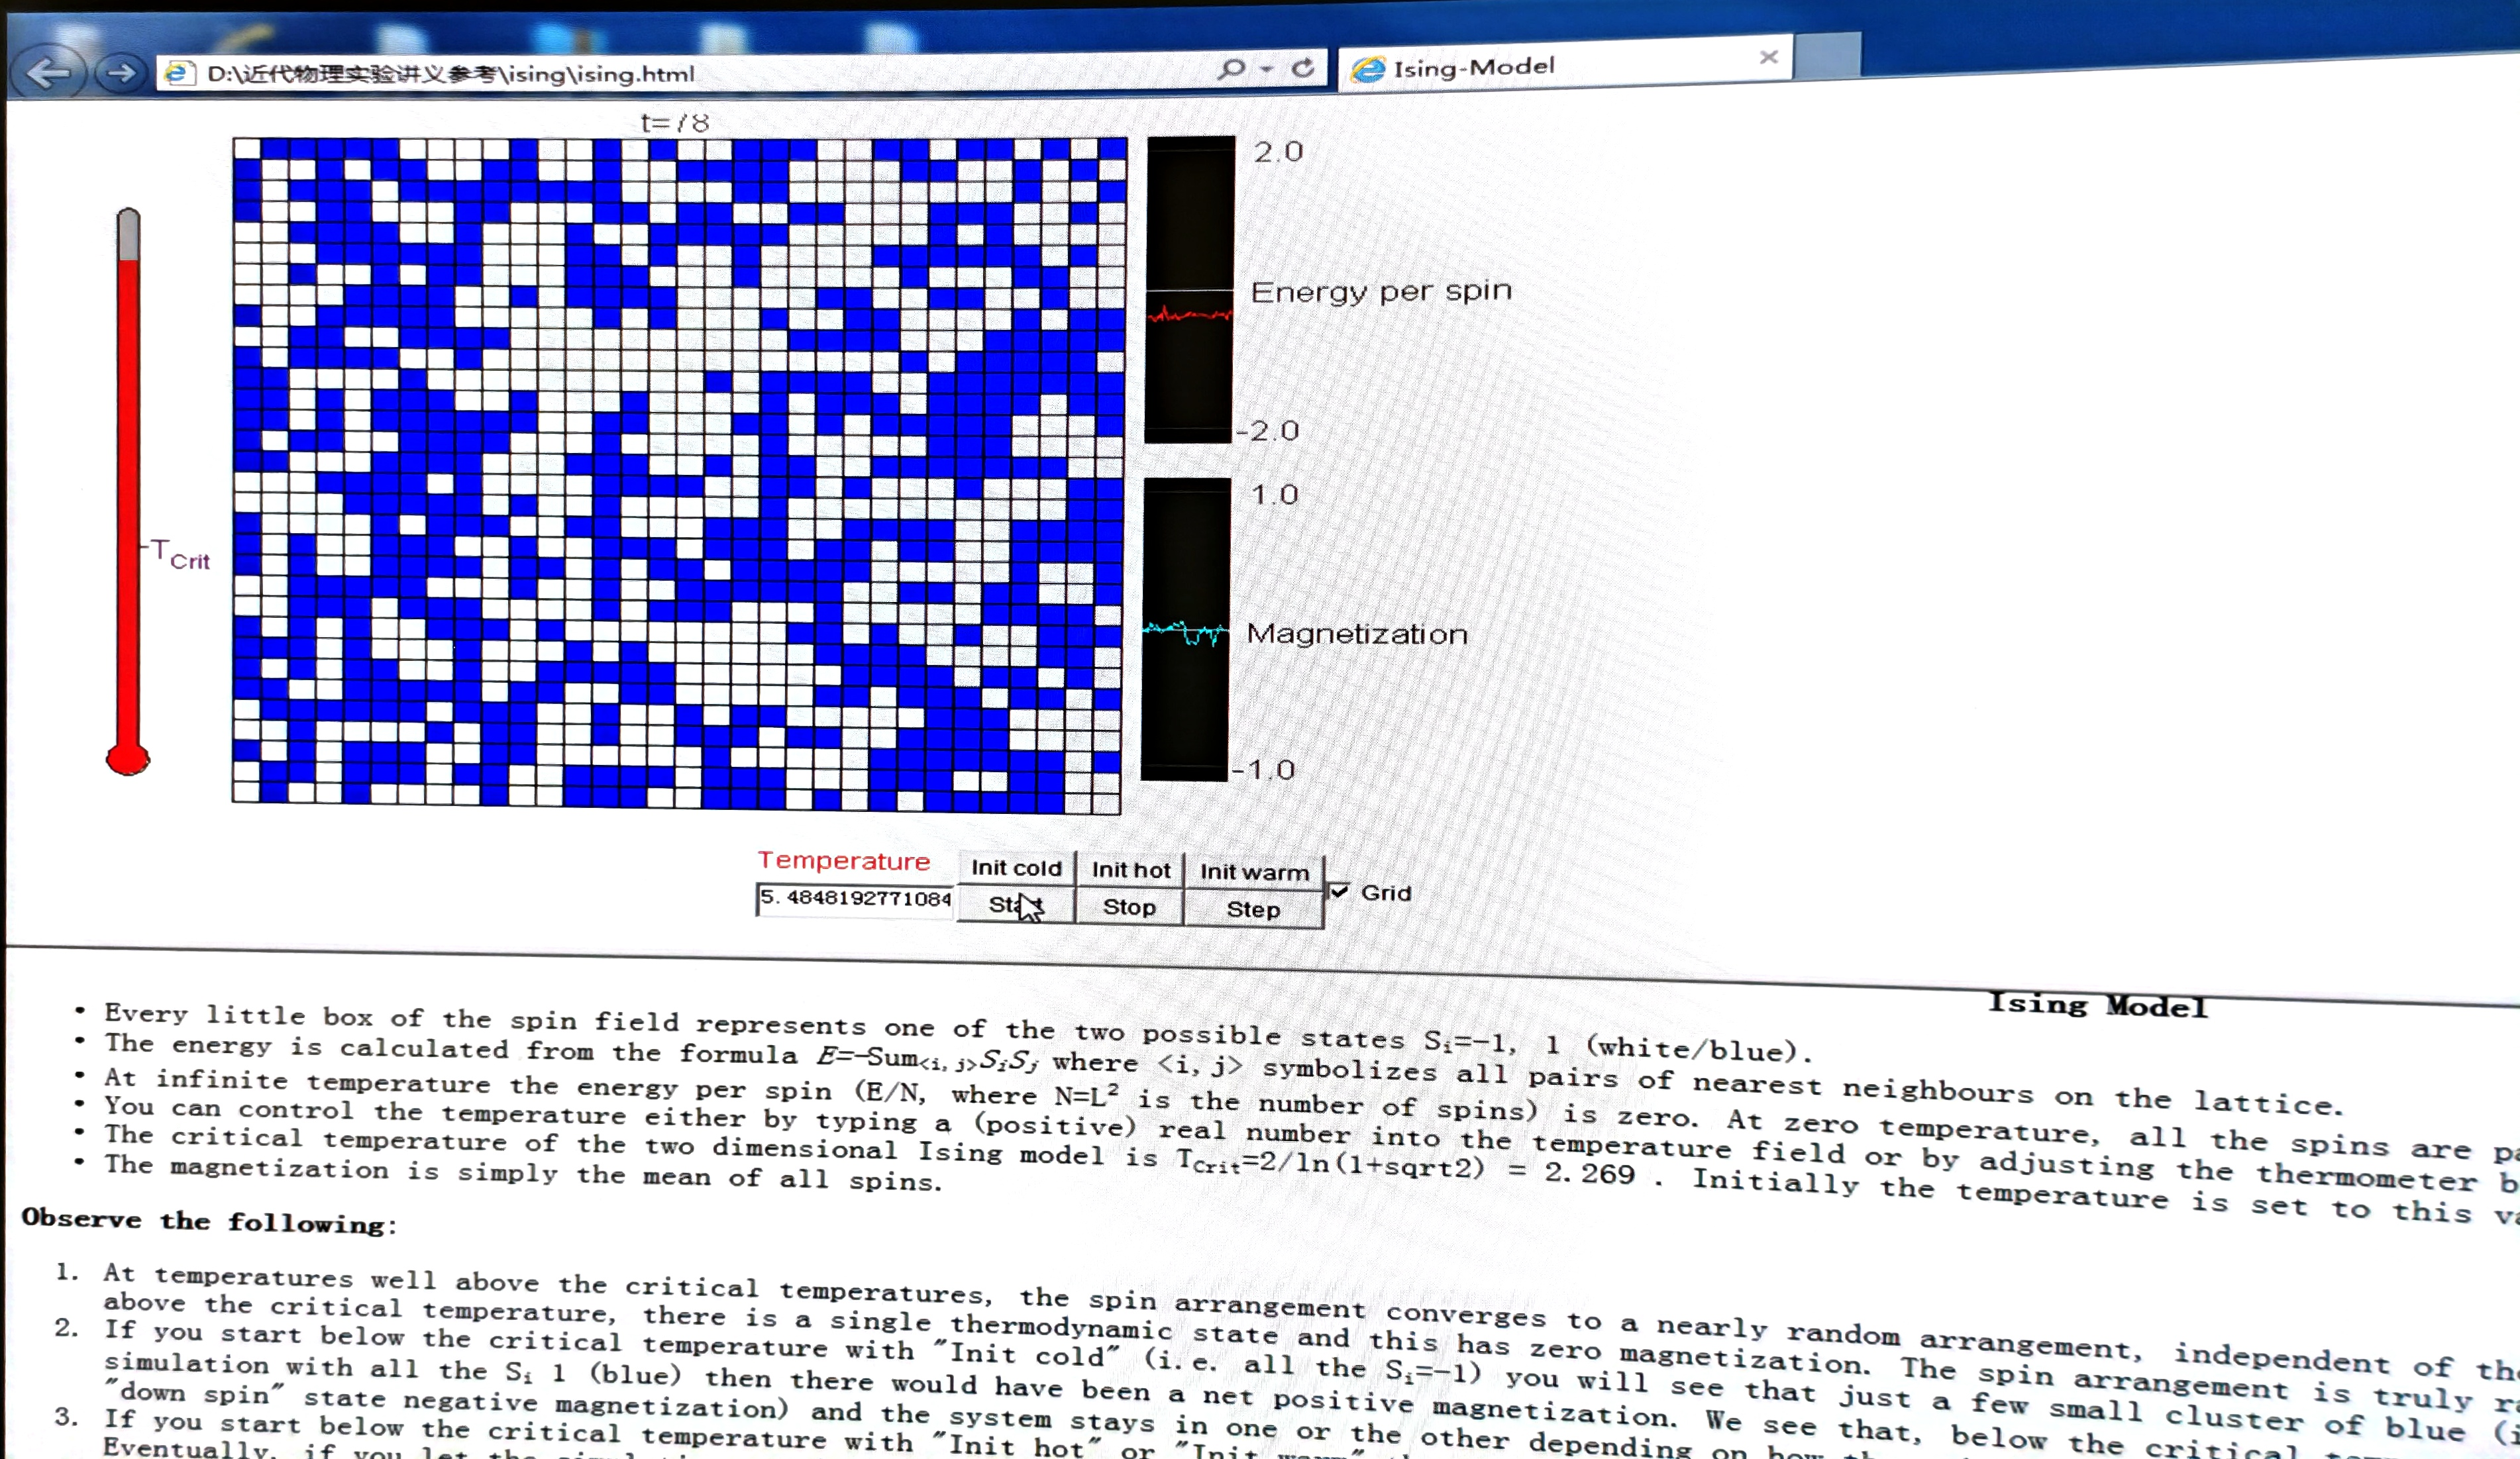
\includegraphics[width=\textwidth]{Figure/fig21.jpg}
        \caption{格点 $L=16$ 下的涨落响应函数峰值图}
    \end{subfigure}
    \hfill
    \begin{subfigure}[b]{0.32\textwidth}
        \centering
        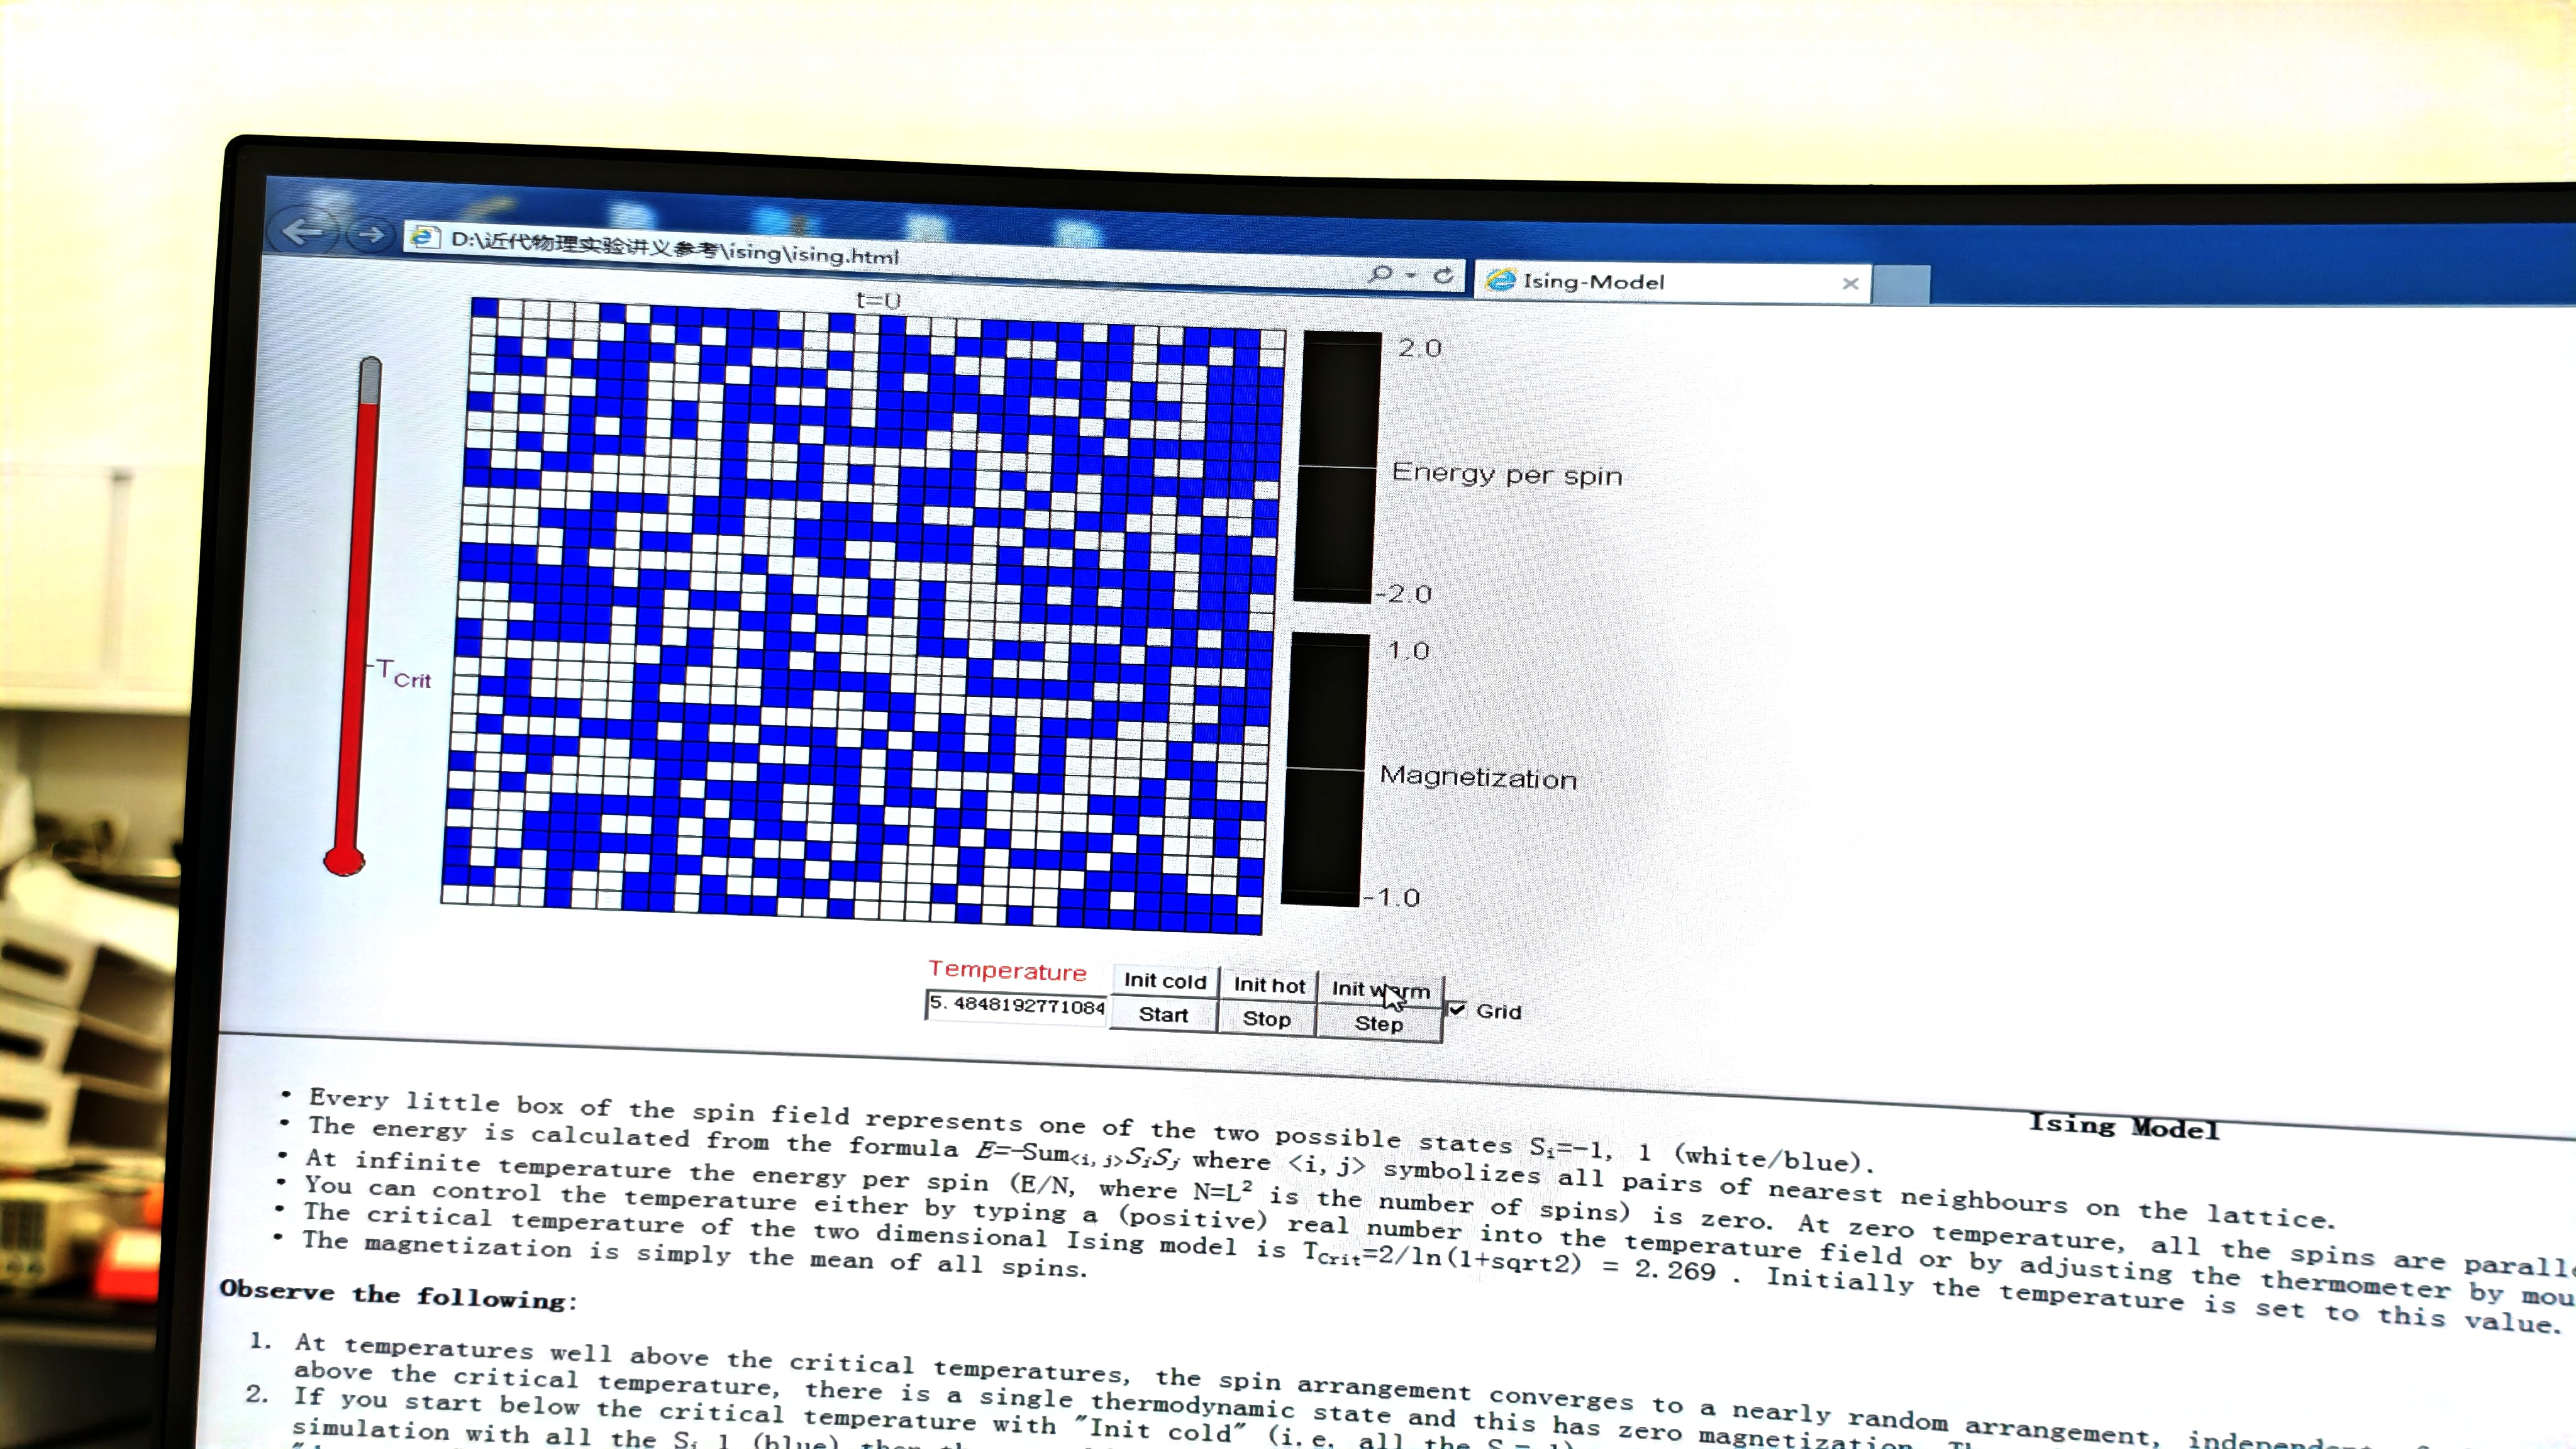
\includegraphics[width=\textwidth]{Figure/fig22.jpg}
        \caption{格点 $L=32$ 下的涨落响应函数峰值图}
    \end{subfigure}
    \hfill
    \begin{subfigure}[b]{0.32\textwidth}
        \centering
        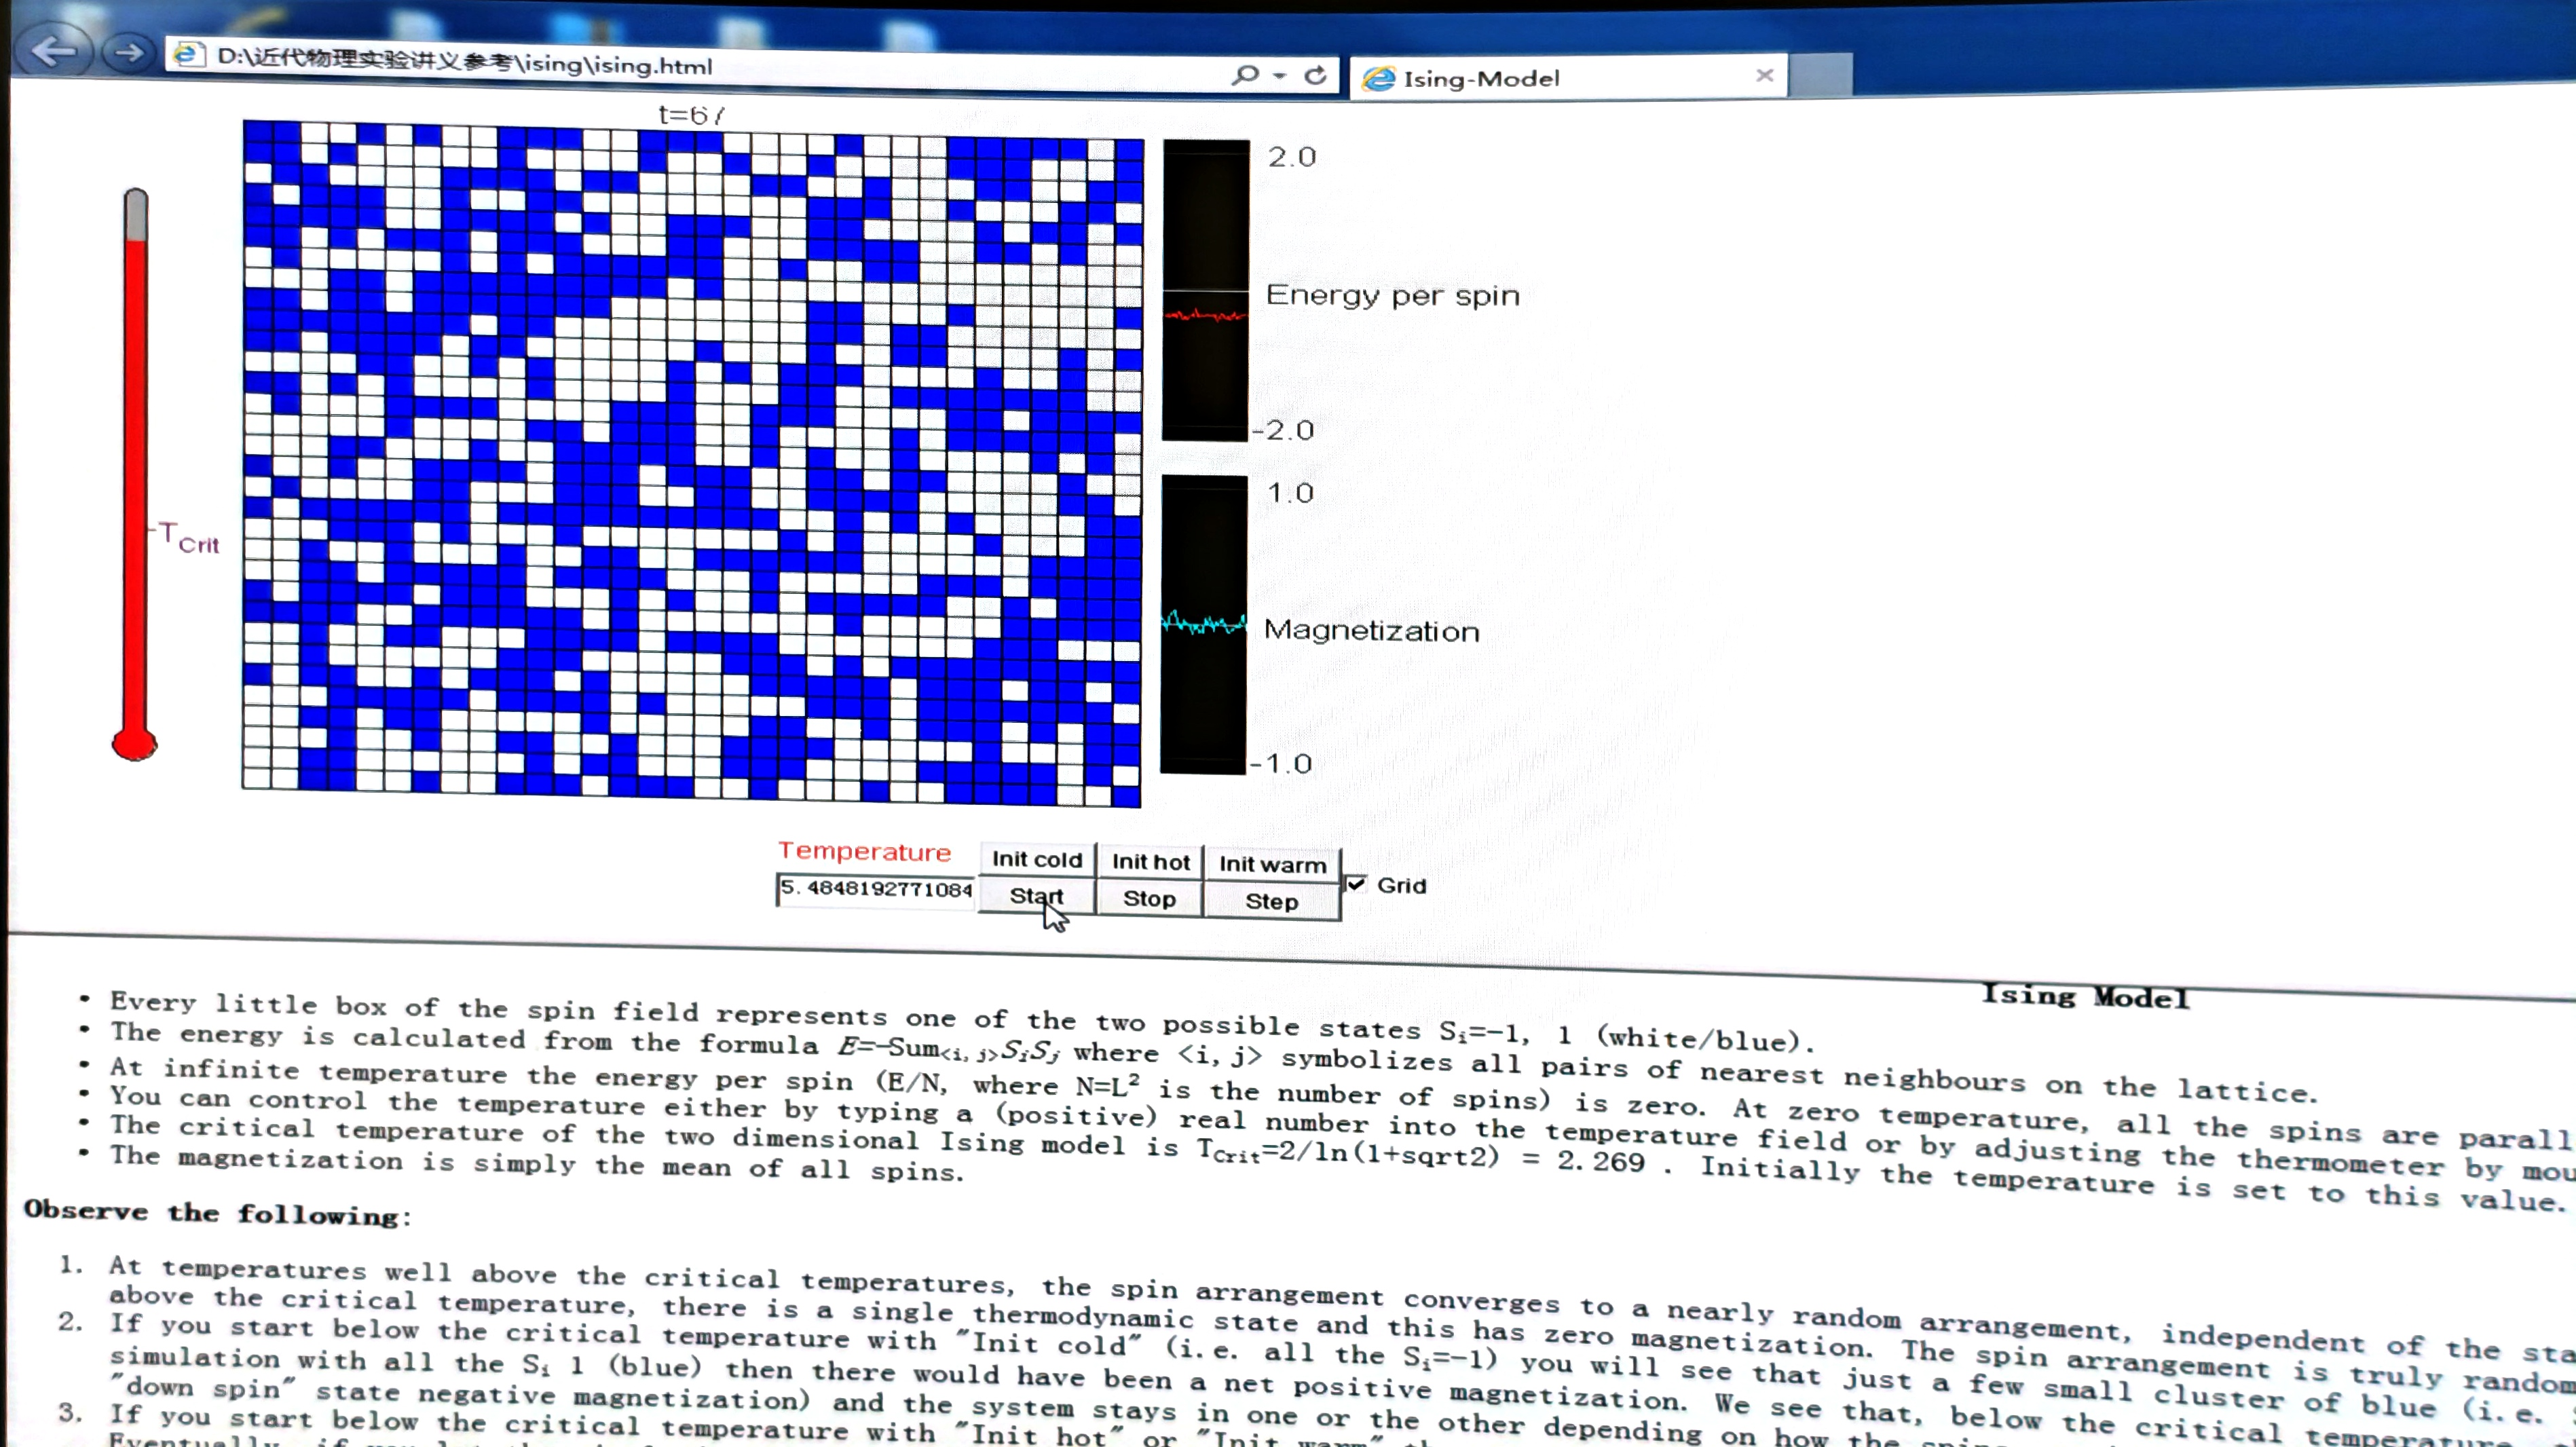
\includegraphics[width=\textwidth]{Figure/fig23.jpg}
        \caption{格点 $L=64$ 下的涨落响应函数峰值图}
    \end{subfigure}
    \caption{体系比热 $C_v$ 与磁化率 $\chi$ 随温度 $T$ 的涨落曲线（展示了在临界相变点附近的峰值发散现象）}
    \label{fig:cv_chi_vs_temp}
\end{figure}

对图 \ref{fig:cv_chi_vs_temp} 涨落响应曲线的物理分析如下：
\begin{enumerate}
    \item \textbf{涨落与响应的关联}：磁化率 $\chi$ 和比热 $C_v$ 均在临界温度附近出现尖锐峰值。物理上，这是因为在临界点处自旋方向的无序和有序两相势均力敌，体系的起伏达到最大。
    \item \textbf{有限尺寸效应（Finite-Size Scaling）}：
        \begin{itemize}
            \item \textbf{峰值高度}：比较 $L=16, 32, 64$ 三组图可以发现，随着晶格网格 $L$ 的增大，比热峰和磁化率峰的**高度显着增加，半高宽显着变窄**。在宏观无限大热力学极限（$L \to \infty$）下，这些峰值将理论上直接发散至无穷大。
            \item \textbf{相变温度移动}：随着 $L$ 的变大，峰值对应的中心温度（数值测量出的临界点 $T_c(L)$）逐渐向左偏移，进一步靠近理论解析解 $T_c^\infty = \frac{2}{\ln(1+\sqrt{2})} \approx 2.269$。本实验中，$L=64$ 时峰值中心在 $T \approx 2.27 \pm 0.01$ 处，已经与理论严格 Onsager 解非常契合。
        \end{itemize}
\end{enumerate}

\section{思考题}

\begin{enumerate}
    \item \textbf{问题：为什么在蒙特卡罗模拟中必须引入周期性边界条件（Periodic Boundary Conditions）？如果采用自由边界条件（Open Boundary Conditions），对模拟得到的相变行为会有什么影响？}
    
    \textbf{解答}：
    在计算机模拟中，受限于计算资源，我们模拟的晶格网格尺寸（如 $L=16$ 或 $32$）通常非常小。如果使用自由边界条件，格点阵边缘上的磁针最近邻个数不再是 4 个（边界处是 3 个，角上是 2 个），这种“表面缺陷”会产生显着的边界截断效应。边界格点感受到的交换相互作用约束小于内部格点，因此更容易因热扰动发生翻转。这会导致系统在比真实临界点更低的温度下就发生自发磁化的崩溃，不仅测得的临界温度 $T_c(L)$ 偏低，而且会极大地抹平相变拐点，甚至抑制相变的发生。
    
    引入周期性边界条件后，格点阵的首尾相互衔接（在拓扑上形成一个二维环面），所有的格点都处于完全等价的物理环境中，最近邻格点数恒为 4 个。这样就消除了任何边界效应的干扰，使我们能够用较小尺寸的格点阵极其成功地逼近无限大系统的宏观热力学行为。

    \item \textbf{问题：请解释在临界温度附近模拟时出现的“临界慢化”（Critical Slowing Down）现象的微观机制，并简述有何改进算法可以克服该问题？}
    
    \textbf{解答}：
    在临界点 $T \approx T_c$ 附近，体系的空间关联长度 $\xi$ 会趋于发散：
    \begin{equation}
        \xi \propto |T - T_c|^{-\nu}
    \end{equation}
    这表明系统内部自旋的运动高度协同，演化出了极其巨大的分形自旋畴。由于本实验使用的 Metropolis 算法是一种**单自旋翻转算法**，每一次翻转操作都只是随机尝试改动单个自旋。而在临界畴块内部，大片自旋方向高度统一，如果单独翻转其中一个自旋，它会被 4 个反向的强近邻包围，系统势能 $\Delta E$ 极大增加，从而根据 Metropolis 条件极难被接受。因此，大块畴结构要想发生状态改变，只能依靠边界格点以极低的概率缓慢游走，导致系统特征弛豫时间（马尔可夫链的去关联时间） $\tau$ 剧烈发散：
    \begin{equation}
        \tau \propto \xi^z \propto |T - T_c|^{-z\nu}
    \end{equation}
    其中 $z \approx 2.17$ 是 Metropolis 算法的临界动力学指数。系统需要耗费极其巨大的蒙特卡罗步数才能过渡到一个新的独立构型，导致采样效率极其低下。
    
    要克服这一难题，可以引入**集体（聚类）翻转算法（Cluster Algorithms）**，如 **Wolff 算法** 或 **Swendsen-Wang 算法**。这些算法不是单个翻转自旋，而是通过链键连接概率将关联的近邻自旋归为一个“畴簇”（Cluster），然后以 100\% 的概率一次性将整个自旋畴簇翻转，其动力学指数 $z$ 近乎为 0。这极大地克服了临界慢化，让临界温度下的采样效率提升数个数量级。

    \item \textbf{问题：对于有限大小的二维 Ising 模型网格，为什么比热 $C_v$ 和磁化率 $\chi$ 的测量峰值不会真正发散到无穷大？我们应如何估算宏观无限大晶格的真实相变临界温度 $T_c^{\infty}$？}
    
    \textbf{解答}：
    在宏观无限大热力学极限下，相变点处的配分函数存在非解析性，导致比热和磁化率等二阶导数响应函数真正发散至无穷大。然而，在有限大小 $L \times L$ 的模拟体系中，自旋关联长度 $\xi$ 被强行截断在晶格尺寸 $L$ 级别，不可能真正发散到无穷大。由于配分函数是有限项指数求和的解析函数，因此任何热力学量的统计平均值及微商都只能表现为有限的平滑峰值，不会出现无限大突变，这是**有限尺寸截断效应**的必然结果。
    
    为了估算无限大系统的真实相变温度 $T_c^{\infty}$，可以利用**有限尺寸标度律（Finite-Size Scaling, FSS）**。根据标度假说，有限大小体系的视在相变温度（即峰值中心点） $T_c(L)$ 满足如下幂律关系：
    \begin{equation}
        T_c(L) - T_c^\infty \propto L^{-1/\nu}
    \end{equation}
    其中，二维 Ising 模型的临界指数解析值为 $\nu = 1$。
    因此，我们可以模拟一系列不同尺寸的 $L$ 值（如 $L=8, 16, 32, 64$），记下各尺寸下比热或磁化率峰值的温度中心点 $T_c(L)$。然后，以 $T_c(L)$ 为纵轴、 $1/L$ 为横轴进行线性外推。当 $1/L \to 0$（即 $L \to \infty$）时的截距，即为高精度估算出的无限大晶格真实热力学临界相变温度 $T_c^{\infty}$。
\end{enumerate}

\end{document}